\documentclass[honors]{union-cs-thesis}

\usepackage{fullpage}
\usepackage{url}
\usepackage{todonotes}
\usepackage{amsmath}
\usepackage{amsthm}
\usepackage{amsfonts}
\usepackage{amssymb}
\usepackage[utf8]{inputenc}
\usepackage{soul}
\usepackage{multicol}
\usepackage[numbers]{natbib}
\usepackage[ruled, vlined, linesnumbered]{algorithm2e}
\usepackage{placeins}
\usepackage{caption}
\usepackage[position=top]{subcaption}
\usepackage{listings}
\usepackage{pgfplots}
\usepackage[toc,page]{appendix}
\usepackage{hyperref}
\usepackage[capitalise, noabbrev]{cleveref} % Must be loaded after hyperref

\pgfplotsset{compat=1.3}
\usetikzlibrary{pgfplots.external}
%\tikzexternalize[prefix=tikz/]

% Theorem and Math macros borrowed from 
% CS Professor Matt Anderson
% ------- Theorem and related environments --------
\newtheorem{theorem}{Theorem}
\newtheorem{conjecture}{Conjecture}
\newtheorem{proposition}{Proposition}
\newtheorem{claim}{Claim}
\newtheorem{lemma}{Lemma}
\newtheorem{corollary}{Corollary}
\newtheorem{definition}{Definition} 
\newtheorem{problem}{Problem}
\newtheorem{observation}{Observation}
\newtheorem{fact}{Fact}

\newcommand{\NN}{\mathcal{N}} % Natural Numbers
\newcommand{\RR}{\mathcal{R}} % Real Numbers
\newcommand{\ZZ}{\mathcal{Z}} % Integers
\newcommand{\QQ}{\mathcal{Q}} % Rational Numbers

\newcommand{\set}[1]{\ensuremath{\{{#1}\}}} % Set
\newcommand{\bigset}[1]{\ensuremath{\left\{{#1}\right\}}}
\newcommand{\condset}[2]{\ensuremath{\set{{#1}\;|\;{#2}}}} % Conditional set
\newcommand{\nin}{\not\in}
\newcommand{\cross}{\times} % Cartesian product
\newcommand{\ssn}{\subsetneq} % Proper subset
\newcommand{\sse}{\subseteq} % Subset

\DontPrintSemicolon
\newcommand{\spa}{\rightsquigarrow}
\newcommand{\td}{\todo[inline]}

\begin{document}
% Set code listing settings
\lstset{
    language=Java,
    basicstyle={\scriptsize, \linespread{0.8}},
    frame=single,
    numbers=left,
    showstringspaces=false,
    stringstyle=\ttfamily,
    breaklines=true,
    caption=\texttt{\lstname}
} 


\pagenumbering{roman} % Roman numeral page numbers in table of contents

\title{Iterated Local Search Algorithms for Bike Route Generation}
\author{Aidan R. Pieper}
\date{\today}

% The three commands below are only used when the honors option is
% passed to \documentclass.  
\authorLF{Pieper, Aidan R.}
\dept{Department of Computer Science}
\advisor{Matthew Anderson}

\maketitle

\begin{abstract}
\makeabstract

Planning routes for recreational cyclists is challenging because they prefer longer more scenic routes, not the shortest one. This problem can be modeled as an instance of the Arc Orienteering Problem (AOP), a known NP-Hard optimization problem. Because no known algorithms exist to solve this optimization problem efficiently, we solve the AOP using  heuristic algorithms which trade accuracy for speed. We implement and evaluate two different Iterated Local Search (ILS) heuristic algorithms using an open source routing engine called GraphHopper and the OpenStreetMap data set. We propose ILS variants which our experimental results show can produce better routes at the cost of time. 

\end{abstract}

\tableofcontents
\listoffigures % empty if using condensed formatting
\listoftables % empty if using condensed formatting
\lstlistoflistings
\makepreamble

\pagenumbering{arabic}

\section{Introduction}
Cycling is a popular and diverse activity enjoyed by millions of people all over the world. To some, cycling is a means of commuting to work while to others it is a recreational sport.  The quality of cycling infrastructure varies across the globe. In countries like Belgium and the Netherlands where cycling is a popular recreational sport, there are vast networks of bicycle-friendly secondary roads \cite{souffriau2011planning}. However, many places do not have this same level of cycling infrastructure so bike riders must share highways with other road vehicles.

Route planning for recreational cyclists poses a fundamentally different problem than traditional route planning problems because the shortest route is not necessarily the 	preferable cycling route. Recreational cyclists generally prefer longer, more scenic, and less trafficked routes as the goal of the activity is recreation not transportation. When planning routes, recreational cyclists consider different factors such as route distance, elevation gain, maximum percent gradient, and how pleasant a road is to travel by bike. Designing a route that fits all user-specified criteria is a difficult task.  Moreover, there are no set criteria which determine a ``preferable" cycling route. The desirability of a given route is based on the rider's personal preferences, goals, and fitness. This research explores different algorithms for generating cycling routes for recreational road cyclists.


Most bike rides begin and end in the same location. Using this assumption, this research focuses specifically on generating preferable \emph{circular} cycling routes. For example, a cyclist may want a 15-mile route which starts and ends at their home.
    

\subsection{Motivations}
Traditional route planning problems focus mainly on finding a path in a graph optimizing for either shortest distance or time. There exists many route planning tools such as \href{https://www.strava.com/routes/new}{\url{strava.com}}, \href{https://www.mapmyride.com}{\url{mapmyride.com}}, and \href{https://ridewithgps.com}{\url{ridewithgps.com}} which allow users to add points on a map and generate a route between such destinations. However, none of these tools can fully generate a route without additional user input.

%\td{Add info about traveling cyclists}


\subsection{Related work} \label{sec:relatedwork}
In the literature, planning preferable cycling routes is modeled as an instance of the Arc Orienteering Problem (AOP), a variant of the Orienteering Problem (OP) \cite{souffriau2011planning}. First introduced in 1987 by \citeauthor{golden1987orienteering}, the classical OP is a combination of node selection and determining shortest paths between nodes in a graph \cite{golden1987orienteering}. The OP is a hybrid between two classical combinatorial problems, the Knapsack Problem and the Traveling Salesman Problem\footnote{The OP may sometimes be referred to as the \emph{Selective} Traveling Salesman Problem \cite{laporte1990selective}.}. In the classical OP, each node in the graph is assigned a non-negative score and a non-negative cost. Given a starting node, a destination node, and some maximum cost budget, the objective is to determine a non-repeating path which starts at the starting node, visits some subset of the graph nodes, and ends at the destination node \cite{gunawan2016orienteering}. In addition, the solution path must both maximize the total collected score, accrued from visiting a node, and keep the total collected cost under the specified budget.

The AOP is the arc variant of the OP where each arc, i.e., graph edge, is given a score and a cost. In the AOP, scores and costs are accrued from visiting an arc instead of a node. For example, \cref{fig:aop-example} shows an undirected AOP instance where $S$ is the start node, $D$ is the destination node, the budget is 10, and every edge is labeled (score, cost). The shortest path is $S \rightarrow (10,3) \rightarrow (5,5) \rightarrow D$ which has a cost of 8 and a score of 15. However, for the specified budget, $S \rightarrow (20,1) \rightarrow (3,2) \rightarrow (2,2) \rightarrow (5,5) \rightarrow D$ is the optimal solution with a score of 30 and a cost of 10. The optimal solution is clearly not the shortest path but rather the path with the maximal score constrained by the cost budget.

Previous research shows that both the OP and the AOP are NP-Hard problems for directed and undirected graphs \cite{gunawan2016orienteering}. No algorithms are known to \emph{optimally} solve the AOP or OP in polynomial time. While there is considerable research into the OP and its variants, there is less research into the AOP. \citeauthor{gunawan2016orienteering} provide an exhaustive survey of the OP and its variants, but the AOP is clearly over shadowed by other OP variants in the literature \cite{gunawan2016orienteering}.

\begin{figure}
\begin{center}
    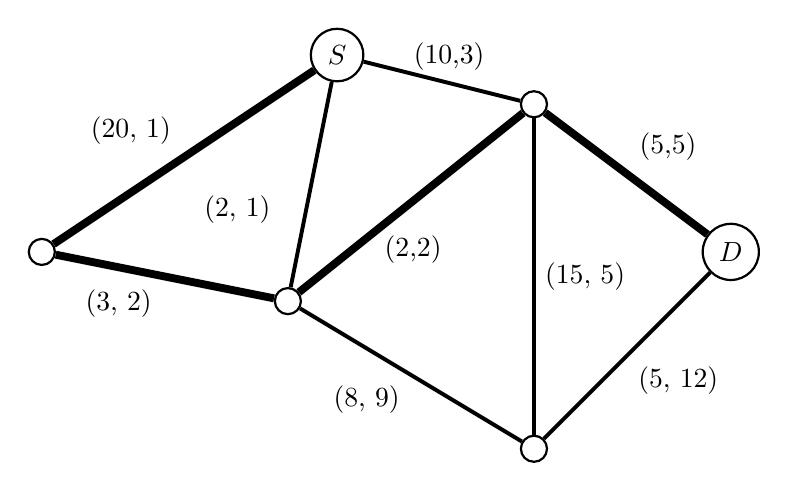
\begin{tikzpicture}[auto,x=1.25cm, y=1.25cm,line width=0.5mm]
    
        \begin{scope}[every node/.style={circle,thick,draw}]
        \node(1) at (0,0) {$S$};
        \node(2) at (2, -0.5) {};
        \node(3) at (4, -2) {$D$};
        \node(4) at (2, -4) {};
        \node(5) at (-0.5, -2.5) {};
        \node(6) at (-3, -2) {};
        \end{scope}
        
        \draw (1) -- node[xshift=-0.5cm] {(10,3)} (2);
        \draw[line width=1mm]  (2) -- node {(5,5)} (3);
        \draw (3) -- node {(5, 12)} (4);
        \draw (2) -- node {(15, 5)} (4);
        \draw[line width=1mm] (2) -- node[yshift=-0.25cm, xshift=-0.5cm] {(2,2)}(5);
        \draw (4) -- node {(8, 9)}(5);
        \draw[line width=1mm] (5) -- node {(3, 2)} (6);
        \draw[line width=1mm] (6) -- node[] {(20, 1)} (1);
        \draw (1) -- node [xshift=-1.5cm]{(2, 1)} (5);
    
    \end{tikzpicture}
\end{center}
\caption[Undirected AOP instance]{Undirected AOP instance with start node $S$ and destination $D$. Arc label is (score, cost). Bold path is optimal for a budget of 10 (score = 30, cost = 10).\label{fig:aop-example}}
\end{figure}

 
\citeauthor{gavalas2015approximation} \cite{gavalas2015approximation} show approximation algorithms for the AOP in both directed and undirected graphs. Approximation algorithms are algorithms to NP-Hard optimization problems that do not produce optimal answers yet have provable accuracy bounds. A polylogarithmic approximation algorithm is shown for directed graphs while a $(6 + \epsilon + o(1))$-approximation algorithm is shown for undirected graphs \cite{gavalas2015approximation}. Moreover, they show a reduction from the AOP to the OP. Using an existing OP approximation algorithm by \citeauthor{nagarajan2011directed} \cite{nagarajan2011directed}, this reduction yields a $O(\frac{(\log m)^2}{\log \log m})$-approximation algorithm for solving the AOP in directed graphs where $m$ is the number of edges.

\citeauthor{souffriau2011planning} \cite{souffriau2011planning} study the AOP in the context of cycle trip planning. \citeauthor{souffriau2011planning} provide an integer programming mathematical model for the AOP and a greedy randomized adaptive search heuristic algorithm for solving AOP instances to near optimality in a few seconds. To evaluate performance of their algorithm, the authors test their algorithm against a road network of bike-friendly roads in East Flanders. The East Flanders' bicycle road network covers 5 regions and is comprised of 989 nodes with 2963 arcs for a total of 3585 km of road. This model for the AOP requires that each node and edge is visited at most once by the solution path.

\citeauthor{verbeeck2014extension} \cite{verbeeck2014extension} consider the cycle trip planning problem in a directed graph. The authors propose two heuristic algorithms for solving the AOP: A branch-and-cut algorithm and an iterated local search algorithm. See \cref{sec:ils} for a detailed explanation of iterated local search. Unlike, \citeauthor{souffriau2011planning}, this model allows the route to visit the same vertex multiple times but visiting the same arc twice is not allowed. A two-way road can be travelled exactly once in each direction since it is modeled by two separate edges in the directed graph.  Both algorithms were evaluated by running them on the East Flanders road network dataset provided by \citeauthor{souffriau2011planning}

Similarly, research by \citeauthor{bergman2015optimization} \cite{bergman2015optimization} defines the ``Circular Cycle Tour Problem" as a cycle trip planning problem where the start and end location are the same. Like other cycle routing problems, they model it as an instance of the AOP. \citeauthor{bergman2015optimization} use a popularity weighted road network graph using road popularity data from smartphone fitness tracking application \href{http://www.sports-tracker.com/}{\url{sports-tracker.com}}. The authors use a tabu search heuristic algorithm for solving their AOP instance.


\subsection{Research Question}
As mentioned in \cref{sec:relatedwork}, existing literature models cycle trip planning as an instance of the AOP. This research follows the existing literature and focuses on implementing and improving existing AOP algorithms for cycle route planning. 

Since road networks can be quite large and because the AOP is NP-Hard, searching for the optimal route may take an infeasible amount of time. Since we care more about finding a good route than finding the best possible route, we trade off optimality for speed. However, even AOP approximation algorithms are too slow for applications where a response time on the order of milliseconds is required, e.g., 300 ms \cite{lu2015arc}. Therefore, we focus on heuristic algorithms for route generation. Both \citeauthor{verbeeck2014extension} and \citeauthor{lu2015arc} propose heuristic algorithms which follow the Iterated Local Search (ILS) framework. ILS is a heuristic method for solving many optimization problems. ILS builds a sequence of locally optimal solutions through repeated applications of a heuristic search algorithm. Our research question is as follows:

\begin{quote}
    \emph{To what extent can ILS algorithms be improved to generate better bike routes?}
\end{quote}

\subsection{Our Contribution}
In the following sections we refer to the the algorithm proposed by \citeauthor{verbeeck2014extension} as the \emph{VVA Algorithm} and the algorithm proposed by \citeauthor{lu2015arc} as the \emph{LS Algorithm}. We implement the VVA and LS algorithms using an open source routing engine named GraphHopper. We make initial observations by running these algorithms on a subset of the New York State road network using public mapping data from the OpenStreetMap foundation. These observations lead us to create four variants of the LS algorithm. We then ran experiments on a small road network to compare the relative performance of VVA, LS, and our variants. We also pursue an absolute algorithm evaluation by attempting solve an Integer Program model of the AOP. 

Our experimental results show that the LS algorithm is faster than the VVA algorithm but not substantially. However, the LS algorithm does produce substantially higher scoring routes than VVA. Our LS variants can produce even higher scoring routes than the baseline LS algorithm but at a cost of time. We are unable to validate the claimed 300 millisecond response time of the LS algorithm. VVA and LS are solving slightly different problems since VVA restricts taking a road more than once while LS does not. This may account for the scoring differences.

The remainder of this thesis explains this research in detail. \cref{sec:prelim} contains background information on ILS, VVA, and LS. Next, \cref{sec:ils-implementation} discusses our data source, the open source software we used, and our implementation of VVA and LS including our LS variants. In \cref{sec:data} we present our experimental data and performance analysis using two different ILS stopping criteria. We also discuss an Integer Programming model for the AOP. Finally, we conclude with a summary of our results and future work.

\section{Preliminaries}
\label{sec:prelim}
ILS is a heuristic method for solving many discrete optimization problems. First, we explain the abstract idea of ILS. Then we explain how ILS is used in both the VVA and LS algorithms. The VVA algorithm uses a simple depth-first-search with additional checking. The LS algorithms uses a greedy search with spatial techniques to reduce the search space.
\td{Re-write this intro}

\subsection{Modeling Preferability of Cycling Routes} \label{routefactors}
Recreational cyclists consider many factors when designing a preferable cycling route. The following is a non-exhaustive list of such factors:

\begin{multicols}{3}
\begin{itemize}
    \item Route distance
    \item Route elevation gain
    \item Time
    \item Maximum percent gradient
    \item Amount of traffic
    \item Number of intersections
    \item Good cellular service
    \item Easy parking at start
    \item Availability of restrooms
    \item Availability of rest stops
    \item Scenery
    \item Proximity to bike shops
    \item Proximity to mass transit
    \item Limited uphill at end of ride
\end{itemize}    
\end{multicols}

Many of these factors can be modeled nearly identically. For example, distance, elevation gain, and time are all calculated by the sum of those weights over all roads in the route. On the other hand, maximum percent gradient can be seen as a ``Boolean criterion." That is, a road's steepness is either under the maximum percent gradient or over, in which case the road does not satisfy this criterion. If these Boolean criteria must be avoided, a simple option is to initially remove all roads from the graph which do not meet these criteria.

In previous research, the cost of a particular arc is usually the length of the road and the score is some measure of the preferability of the road. Since the AOP requires a single value for the cost and score of each arc, computing costs and scores as linear combinations of different features is a one way to model multiple factors. For example, a particular road's cost might be a combination of its length, its elevation gain, and the level of traffic on the road. This allows one to give certain factors more importance by weighting them more heavily in the linear combination. Furthermore, one might want to avoid certain Boolean criteria instead of outlawing them entirely. For instance, one could avoid dirt roads by giving them higher costs.

While multiple route factors are important to recreational cyclists, the focus of this research is not to model the preferability of roads. Hence, we assume that we have the necessary data to appropriately score roads for recreational cyclists. The focus of this research is on the route planning algorithm, not creating the graph and its associated weights which represents the AOP instance.

\subsection{Iterated Local Search}
\label{sec:ils}
Iterated Local Search (ILS) is a framework for solving optimization problems using heuristic search algorithms. A heuristic is a technique used to solve a problem quickly when exact or approximation methods are too slow. Heuristic algorithms can be thought of as ``shortcuts" in that they trade optimality and completeness for speed. Heuristics are often used in search algorithms to  determine which branch of the search to take but are not guaranteed to produce the best solution. A heuristic algorithm is commonly referred to as a heuristic.

Local Search is a heuristic method for solving optimization problems. Local Search starts with a candidate solution and moves to a higher scoring solution as defined by an objective function which scores solutions in the search space \cite{gendreau2010handbook}. Local Search can get stuck in local optima which are points in the search space that are better than all neighbors but are not the best possible solution.

ILS is a variant of Local Search that attempts to stop it from getting trapped in local optima. Instead of repeating random trials of the heuristic algorithm, ILS builds a sequence of locally optimal solutions generated by the heuristic which is more likely to lead to a better overall solution \cite{gendreau2010handbook}. This is done by first generating an initial solution using the search heuristic, perturbing the current solution, and applying the search heuristic again on the modified solution. The perturbation and local search steps are then repeated until some condition, usually time, is met.
The following pseudocode outlines the ILS framework:

%
% Iterated Local Search definition
%
\begin{algorithm}
\caption{ILS($t$, $localsearch$, $score$)}
\KwData{$t$: a time, $localsearch$: a heuristic search function, $score$: an objective function, $perturb$: a function which modifies the solution.}
\KwResult{A solution of the $localsearch$ function.}
S $\gets$ $localsearch$(empty solution)\;
\While{$t$ seconds have not elapsed}{
    $S^* \gets perturb(S)$\;
    $S' \gets localsearch(S^*)$\;
    \If{$score(S') > score(S)$}{
        $S \gets S'$\;
    }
}
\KwRet{S}
\end{algorithm}

Despite its simplicity, ILS can be challenging to implement efficiently because many implementation choices are left to the developer. For example, an efficient ILS implementation requires a certain level of domain specific knowledge. The main issue with ILS is that the algorithm may still get ``trapped" in a local maximum over many iterations. Therefore, the modification step must modify the solution enough to make progress but not too much that the search is effectively starting with a different ``random" solution upon each iteration. 

% TODO(Aidan) draw picture of ils peaks and troughs


\subsection{VVA Algorithm}
%\td{The graph $G$ is never passed in anywhere in the pseudocode??}
The local search algorithm proposed by \citeauthor{verbeeck2014extension} is a modified version of depth-first-search (\cref{alg:dfs}). It is implemented as a recursive function which used to to find a path between two disconnected nodes in the bike route. The algorithm is allowed to ``take" an outgoing edge and add it to the current route as long as it has not been traversed before and the shortest path from the end of the traversed arc to the destination is less than the remaining distance budget after taking the arc (\cref{alg:dfs:feasability}). In other words, it must be \emph{feasible} to get from the end of the chosen arc to the desired destination after traversing the arc. 

\begin{figure}
\begin{center}
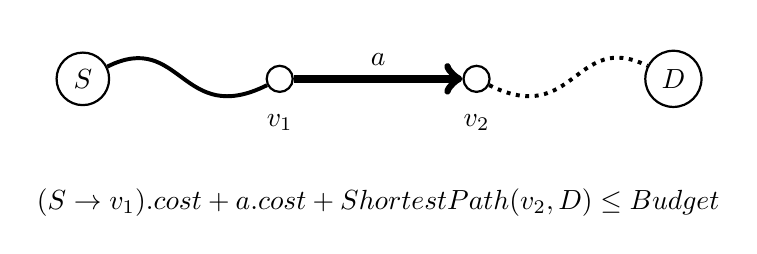
\begin{tikzpicture}[auto,x=1.25cm, y=1.25cm,line width=0.5mm]
    \begin{scope}[every node/.style={circle,thick,draw}]
        \node(1) at (0,0) {$S$};
        \node(2) at (6, 0) {$D$};
        \node[label=below:$v_1$](3) at (2,0) {};
        \node[label=below:$v_2$](4) at (4,0) {};
        \end{scope}
        \draw (1) .. controls (1, 0.5) and (1, -0.5) .. (3);
        \draw[->, line width=1mm] (3) -- node{$a$}(4);
        \draw[dotted] (4) .. controls (5, -0.5) and (5, 0.5) .. (2);
        \node[below] at (3,-1) {$(S \rightarrow v_1).cost + a.cost + ShortestPath(v_2, D) \leq Budget$};
    \end{tikzpicture}
\end{center}
\caption{Arc feasibility checking}
\end{figure}


Since this requires many shortest path computations, the VVA algorithm assumes that all-pairs shortest path have been pre-computed before the ILS runs. In Algorithm \cref{alg:dfs}, the function $shortestPath(v_1, v_2)$ would return the pre-computed shortest path. In addition, the $maxDepth$ parameter is used to restrict the depth of the search and reduce the search space (\cref{alg:dfs:depth}).

\begin{algorithm}
    \caption{DFS($route$, $s$, $d$, $dist$, $minProfit$, $maxDepth$)\label{alg:dfs}}
    \KwData{$route$: a temporary solution, $s$: the start node of the path, $d$: the end node of the path, $dist$: the maximum cost of the route, $minProfit$: the minimum score of the route, $maxDepth$: the maximum number of edges allowed in the solution, $shortestPath(v_1, v_2)$: a function which returns the shortest distance between two nodes of the graph, and $edges(v_1)$: a function which returns all edges of a node. 
        }
    \KwResult{A boolean which denotes whether a path was found. If true, the solution is contained inside of $route$.}
    \If{$maxDepth < 0$}{\label{alg:dfs:depth}
        \KwRet{false}\;
    }
    \For{$arc \in edges(s)$}{ \label{alg:dfs:for}
        \If{$arc \nin route$ and $arc.cost + shortestPath(arc.end, d) < dist$}{\label{alg:dfs:feasability}
            Add $arc$ to $route$\;
            \uIf{$arc.end = d$ and $route.score > minProfit$}{\label{alg:dfs:end}
                \KwRet{true}\;
            } \ElseIf{DFS(route, arc.end, d, dist - arc.cost, minProfit, maxDepth - 1)}{\label{alg:dfs:recurse}
                \KwRet{true}\;
            }
            Remove $arc$ from $route$\;
        }\label{alg:dfs:endfor}
    }
\KwRet{false}\;
\end{algorithm} 

Using this DFS algorithm as the local search heuristic \citeauthor{verbeeck2014extension}, apply the ILS framework to create a bike route planning algorithm. \cref{alg:ils-ver} first generates an initial route using the DFS heuristic and stores the path in the variable $route$ (\cref{alg:ilsv:init}). The ILS perturbs the solution by removing a road from the solution and invoking the DFS procedure to find a new solution (\crefrange{alg:ilsv:perturb}{alg:ilsv:improve}). In the perturbation phase, the algorithm removes $R$ consecutive arcs starting at the arc at position $A$ in solution $route$. If a new path is found after removing a path segment from the solution, then the new path is merged into the current solution (\cref{alg:ilsv:merge}). If no new path with score improvement can be found $A$ and $R$ are both incremented by 1 (\cref{alg:ilsv:increment}). This perturbs the solution more and more in an attempt to move the search out of a local optima.

%
% VVA ILS Algorithm
%
\begin{algorithm}
    \caption{ILS-VVA($s$, $d$, $dist$, $maxDepth$, $t$) \label{alg:ils-ver}}
    \KwData{$s$: the start node of the path, $d$: the end node of the path, $dist$: the maximum distance of the path, $maxDepth$: the maximum depth allowed in the DFS, and $t$: a time.}
    \KwResult{a path.}
    
    $route \gets$ empty route\;
    \If{not DFS(route, s, d, dist, 0, maxDepth)}{\label{alg:ilsv:init}
        $route \gets$ empty route\;
    }
    $A \gets 1$, $R \gets 1$\;
    
    \While{$t$ seconds have not elapsed}{
        $temp \gets$ copy of $route$\;
        \If{$R > temp.length$}{
            $R \gets 1$\;
        }
        
        \If{$A + R > temp.length -1$}{
            $R \gets temp.length - 1 - A$\;
        }
        
    
        Remove $R$ arcs from $temp$ starting at arc at index $A$\; \label{alg:ilsv:perturb}
        $minScore \gets$ sum of scores of removed arcs from $temp$\;
        $s^* \gets$ starting node of first arc removed\;
        $d^* \gets$ ending node of last arc removed\;
        $new \gets$ empty route\;
        
        \If{DFS(new, $s^*$, $d^*$, dist - temp.dist, minScore, maxDepth)}{\label{alg:ilsv:improve}
            Merge $new$ into $temp$ at index $A$\; \label{alg:ilsv:merge}
            $route \gets temp$\;
            $A \gets 1$, $R \gets 1$\;
        } \Else {
            $A \gets A + 1$, $R \gets R + 1$\; \label{alg:ilsv:increment}
        }
    
    }
    
    \KwRet{route}        
\end{algorithm}

The main drawback of the VVA algorithm is that the ILS has slow iteration because it is performing DFS on every iteration.  Moreover, it requires many shortest paths to be precomputed before the algorithm can run. This can be infeasible on large real-world  mapping datasets. Since the algorithm assumes all pairs shortest-path pre-computated, the feasibility checking used by the search is $O(degree^{maxDepth})$ where $degree$ is the average degree of nodes in the road network and $maxDepth$ is the maximum depth allowed in the DFS. However, since the DFS returns when it finds any better path not the best one, this worst case performance is not typically expected.

\subsection{LS Algorithm}
\label{sec:ls-algo}
The ILS algorithm proposed by \citeauthor{lu2015arc} aims to solve many of the problems of VVA including slow iteration and large pre-computation. Instead of relying on pre-computed shortest paths, the LS algorithm uses online shortest path computations but does less feasibility checking by reducing the search space with spatial techniques (See \cref{sec:pruning}). In addition, LS uses a greedy path generation algorithm instead of DFS.

\subsubsection{Attractive Arcs}
LS models a solution route in terms of ``attractive arcs" which are arcs with a positive score. A path from node $v_1$ to $v_2$ is a series of attractive arcs which starts with $a_1$, ends with $a_n$ and is denoted by, $(v_1 \spa a_1 \spa a_2 \spa \ldots \spa a_n \spa v_2)$. The symbol $\spa$ denotes the shortest path in the graph between two nodes or arcs. The path between two adjacent attractive arcs ($a_i \spa  a_{i+1}$) is known as a ``blank path segment" and is the shortest path from the end vertex of $a_i$ to the start vertex of $a_{i+1}$. These vertices are respectively denoted $l_i.start$ and $l_i.end$ where $l_i$ is the shortest path. Given an attractive arc $a_i$ from a solution path, $a_i.pre$ refers to the previous attractive arc ($a_{i-1}$) and $a_i.post$ refers to the next attractive arc in the path ($a_{i+1}$). The total cost of a path is the sum of all costs of all the arcs in the path, including the arcs in the blank path segments. The score of a path is defined similarly. To build a solution, the LS algorithm connects many attractive arcs together using shortest path blank path segments.

\subsubsection{Candidate Arc Set}
Every arc $a$ in the solution $S$ is associated with a set of candidate attractive arcs. Arcs are taken out of these sets in order to generate a path between two vertices.
%
% Definition of Candidate Arc Set
%
\begin{definition}[\cite{lu2015arc}]
    Let $a \in S$ be an arc in the solution $S$ whose distance budget is $B$. Then the Candidate Arc Set (CAS) of $a$, denoted by $a.CAS$ is the set of arcs who have a positive score and can feasibly replace $a$ in $S$, i.e. $\forall a_c \in a.CAS, a_c.score > 0$ and $(a.pre \spa a_c \spa a.post).cost < B - S.cost + (a.pre \spa a \spa a.post)$.
\end{definition}

\citeauthor{lu2015arc} show that candidate arc sets have the following inherited property. This allows the search space to be reduced when computing some CASs since the parent CAS can be restricted.
\begin{lemma}[\cite{lu2015arc}] Let $a$ be an arc. Given $a.CAS$, $\forall a_c \in a.CAS, a_c.CAS \sse a.CAS$.
\end{lemma}

To chose which candidate arcs to add to the solution, \citeauthor{lu2015arc} propose a criterion called ``Quality Ratio" which is defined for an arc from a candidate arc set. The intuition is that arcs with higher value and lower cost will be more likely to improve the solution. In order to determine which arcs to remove from the solution in the ILS perturbation, they propose a criteria called ``Improve Potential". The intuition is that solution arcs with lower scores and more valuable nearby arcs are more likely to improve the solution. See \cref{sec:ls-appendix-heuristics} for more information.

\cref{alg:ils-lu-compcas} performs the feasibility checking to generate a set of candidate arcs which can be used to connect a start node $v_1$ to a destination node $v_2$. The algorithm takes in a set of possible arcs, iterates over each one, and adds the arc to the current CAS only if its score is positive and the distance of the path from $v_1$ to $a$ to $v_2$ is within the specified budget (\crefrange{alg:ils-lu-compcas-for}{alg:ils-lu-compcas-add}). In addition, the Quality Ratio is calculated for the specified arc in the CAS (\cref{alg:ils-lu-compcas-qr}). If the CAS, $A$, passed into the algorithm is non-empty, then it can use the ``CAS inherit" property and filter out arcs whose paths are within the new specified budget. If the CAS passed in is non-empty, then the algorithm will iterate over all arcs in the graph to find the ones which can be feasibly inserted (\crefrange{alg:ils-lu-compcas-if}{alg:ils-lu-compcas-ifend}).


%
% Compute Candidate Arc Set algorithm
%
\begin{algorithm}
    \caption{computeCAS($G$, $A$, $v_1$, $v_2$, $dist$) \label{alg:ils-lu-compcas}}
    \KwData{$G$: the road network graph, $A$: a candidate arc set, $v_1$: start node, $v_2$: destination node, $dist$: allowable budget.}
    \KwResult{A set of candidate arcs.} 
    $CAS \gets \text{empty set}$\;
    \If{$A$ is empty}{ \label{alg:ils-lu-compcas-if}
    $A \gets$ all arcs from $G$\; \label{alg:ils-lu-compcas-ifend}
    }
    \For{$a \in A$}{\label{alg:ils-lu-compcas-for}
        \If(\tcp*[h]{Feasibility checking}){$a.score > 0$ and $(v_1 \spa a \spa v_2).cost \leq dist)$}{
            $a.qr = QualityRatio(v_1, v_2, a)$\; \label{alg:ils-lu-compcas-qr}
            add $a$ to CAS\; \label{alg:ils-lu-compcas-add}
        }
    }
    \KwRet{CAS}
\end{algorithm}


%
% Update Candidate Arc Set algorithm
%
\begin{algorithm}
    \caption{updateCAS($A$, $a$, $v_1$, $v_2$, $newDist$, $oldDist$) \label{alg:ils-lu-updatecas}}
    \KwData{$A$: set of all arcs in the graph, $a$: arc whose CAS needs to be updated, $v_1$: node in current path before $a$, $v_2:$ node in current path after $a$, }
    \KwResult{An updated set of candidate arcs}
    $CAS \gets a.CAS$\;
    \If(\tcp*[h]{Restrict CAS using inherit property}){$newDist < oldDist$}{\label{alg:ils-lu-updatecas-less}
        \For{$e \in a.CAS$}{
            \If{$(v_1 \spa e \spa v_2).cost > newDist$}{
                remove $e$ from $CAS$\; \label{alg:ils-lu-updatecas-lessend}
            }
        }
    } \ElseIf(\tcp*[h]{Expand CAS by checking all edges from graph}) {$newDist > oldDist$}{ \label{alg:ils-lu-updatecas-more}
        \For{$e \in A$}{
            \If{$e \nin CAS$ and $e.score > 0$ and $(v_1 \spa e \spa v_2).cost \leq newDist$}{
                add $e$ to $CAS$\; \label{alg:ils-lu-updatecas-moreend}
            }
        }
    }
    \KwRet{CAS}
\end{algorithm}

\cref{alg:ils-lu-updatecas}'s job is to update the CAS for a particular arc $a$. If arcs are added to the current solution, then its distance changes as well as the remaining budget. For the new arcs added, computing the respective CASs using \cref{alg:ils-lu-compcas} suffices. However, the previous arcs in the solution need to have their CASs changed since the remaining distance budget is now different. \cref{alg:ils-lu-updatecas} takes in two budget values, $newDist$ and $oldDist$. If the new budget is smaller than the old budget, there may be some arcs in our CAS whose paths are too long for the new budget. Therefore, the algorithm employs CAS inheritance and restricts the current CAS by removing the arcs which can no longer be feasibly inserted with the new budget (\crefrange{alg:ils-lu-updatecas-less}{alg:ils-lu-updatecas-lessend}). If the new budget is larger than our old budget, then the algorithm must expand the CAS by checking the feasibility of all arcs in the graph (\crefrange{alg:ils-lu-updatecas-more}{alg:ils-lu-updatecas-moreend}).

%\td{Move the CAS to the appendix??}


\subsubsection{ILS Formulation}
The local search method used by LS is a greedy algorithm. It continuously inserts feasible arcs from a CAS at the closest blank path segment until the budget is exhausted or there are no more CAS arcs. The LS ILS algorithm removes a random arc from the solution using the heuristic scoring metric ``Improve Potential" and uses the greedy local search to fill the gap in the path. If a new path is found, it is inserted into the route and the CAS of each arc is computed or updated accordingly. See \cref{sec:ls-appendix-path} for details on this path generation algorithm and how it is used in the ILS. 


\subsubsection{Spatial Pruning Techniques}\label{sec:pruning}
While LS relies on the ``CAS inherit" property to restrict the search space, it still has to do a lot of processing to generate the initial CAS or update CASs when the budget expands. To address this issue,  \citeauthor{lu2015arc} propose an ``ellipse pruning" technique to reduce the number of arcs which need to be checked.


An ellipse is a curve such that for every point on the curve, the sum of the distances to the two focal points is constant. Consider the scenario where there are two graph nodes $v_1$ and $v_2$ in which the desired path between the two has a budget of $b$. Furthermore, consider the ellipse whose focal points are the two nodes and whose sum of the distances to the two focal points is $b$ (\cref{fig:ellipse}). For all points $p$ on the ellipse $(v_1 \spa p \spa v_2).cost = b$ where the shortest path is the straight line Euclidean distance. Therefore, if there is an arc $a$ which connects $v_1$ to $v_2$ and contains a point $p_o$ outside of the ellipse, we know that $a.cost > b$ since $(v_1 \spa p_o \spa v_2).cost > b$. This criteria is used to prune arcs from the search space when calculating or updating CASs.

\begin{figure}
\begin{center}
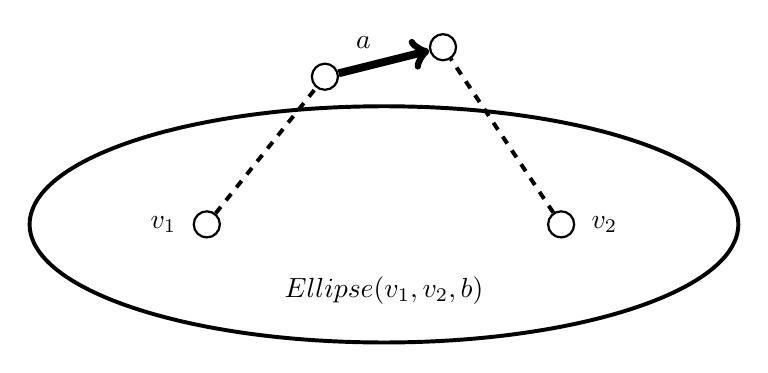
\begin{tikzpicture}[auto, x=1.5cm, y=0.75cm]
  \begin{scope}[every node/.style={circle,thick,draw}]
\node[label=left:$v_1$](1) at (0,0) {};
\node[label=right:$v_2$](2) at (3,0) {};
\node(4) at (1, 2.5) {};
\node(5) at (2, 3) {};
\end{scope}

\draw[dashed, line width=0.5mm] (1) -- (4);
\draw[dashed, line width=0.5mm] (2) -- (5);
\draw[->, line width=1mm] (4) -- node{$a$}(5);

\draw[line width=0.5mm] (1.5, 0) ellipse (4.5 cm and 1.5cm) node [below=15pt] {$Ellipse(v_1, v_2, b)$};
\end{tikzpicture}
\end{center}
\caption{Illustration of \citeauthor{lu2015arc}'s ellipse pruning technique. The goal is to connect $v_1$ to $v_2$ with a path of budget $b$. The arc $a$ is excluded from the search since it contains a point outside of the ellipse and is therefore infeasible. \cite{lu2015arc}.}
\label{fig:ellipse}
\end{figure}



\section{ILS Implementation}
\label{sec:ils-implementation}
We implement the VVA and LS algorithms and evaluate them on real world road networks. This section discusses the technical details of our implementation. We first discuss our data source, the open source software used, and road scoring metrics. Then we explain the choices made in both our VVA and LS implementations. Finally this section concludes with observations of our implementations and we propose four new LS variants based on these observations. 

\subsection{OpenStreetMap}
We use the crowd-sourced open mapping dataset provided by the \emph{OpenStreetMap} (OSM) foundation\footnote{OSM provides a free mapping dataset for the entire planet. A full world map is around 56GB.}\cite{osm}. However, the OSM map format is an XML-based schema which is not trivially translatable into a road network graph. Luckily, in addition to open data, OSM includes a collection of open source software which interface with the data. Because the goal of this research is not to translate raw OSM data into a usable graph representation, we need software that already has this parsing capability in order to implement both ILS algorithms. Because OSM is a crowdsourced dataset, its level of accuracy varies across the world which is the main drawback to using this data. 

\subsubsection{Map Metadata}
Some OSM roads (known as ``ways" in OSM parlance) contain metadata used to help bicycle routing but it is not guaranteed to be available. This bicycle routing hint is a value which is used to express the desirability of a road (\cref{tab:osm-hint}).  
\begin{table}
\begin{center}
    \begin{tabular}{|l|p{0.75\linewidth}|}
        \hline
        \textbf{Metadata Value} & \textbf{Meaning} \\
        \hline
        -3 & ``Avoid at all cost" \\
        \hline
        -2 & ``Only use to reach your destination, not well suited" \\
        \hline
        -1 & ``Better take another way" \\
        \hline
        0 & ``As well as other ways around." \\
        \hline
        1 & ``Prefer" \\
        \hline
        2 & ``Very nice way to cycle" \\
        \hline
        3 & ``This way is so nice, it pays out to make a detour also if this means taking many unsuitable ways to get here." \\
        \hline
    \end{tabular}
\end{center}
\caption{OSM bicycle routing hints. Taken directly from the OSM wiki.}
\label{tab:osm-hint}
\end{table}
However, the OSM wiki notes that these values ``should not be used where other attributes\footnote{Example attributes include number of lanes, maximum speed, and incline.} are considered adequate description" \cite{osm}.

\subsection{GraphHopper}
\label{sec:graphhopper}
We use GraphHopper as the starting point for our research. GraphHopper is an open source routing engine written in Java which can download and parse raw OSM data into a usable graph representation \cite{graphhopper}. On top of data parsing, GraphHopper provides a web server and webpage front-end which are useful for visualizing and running routing algorithms (\cref{tab:graphhopper-frontend}). Internally, GraphHopper has a number of built-in pathfinding algorithms including A* and Dijkstra which can be used for routing. These algorithm implementations provide a good template for implementing other routing algorithms with GraphHopper. 

\begin{figure}
    \begin{center}
        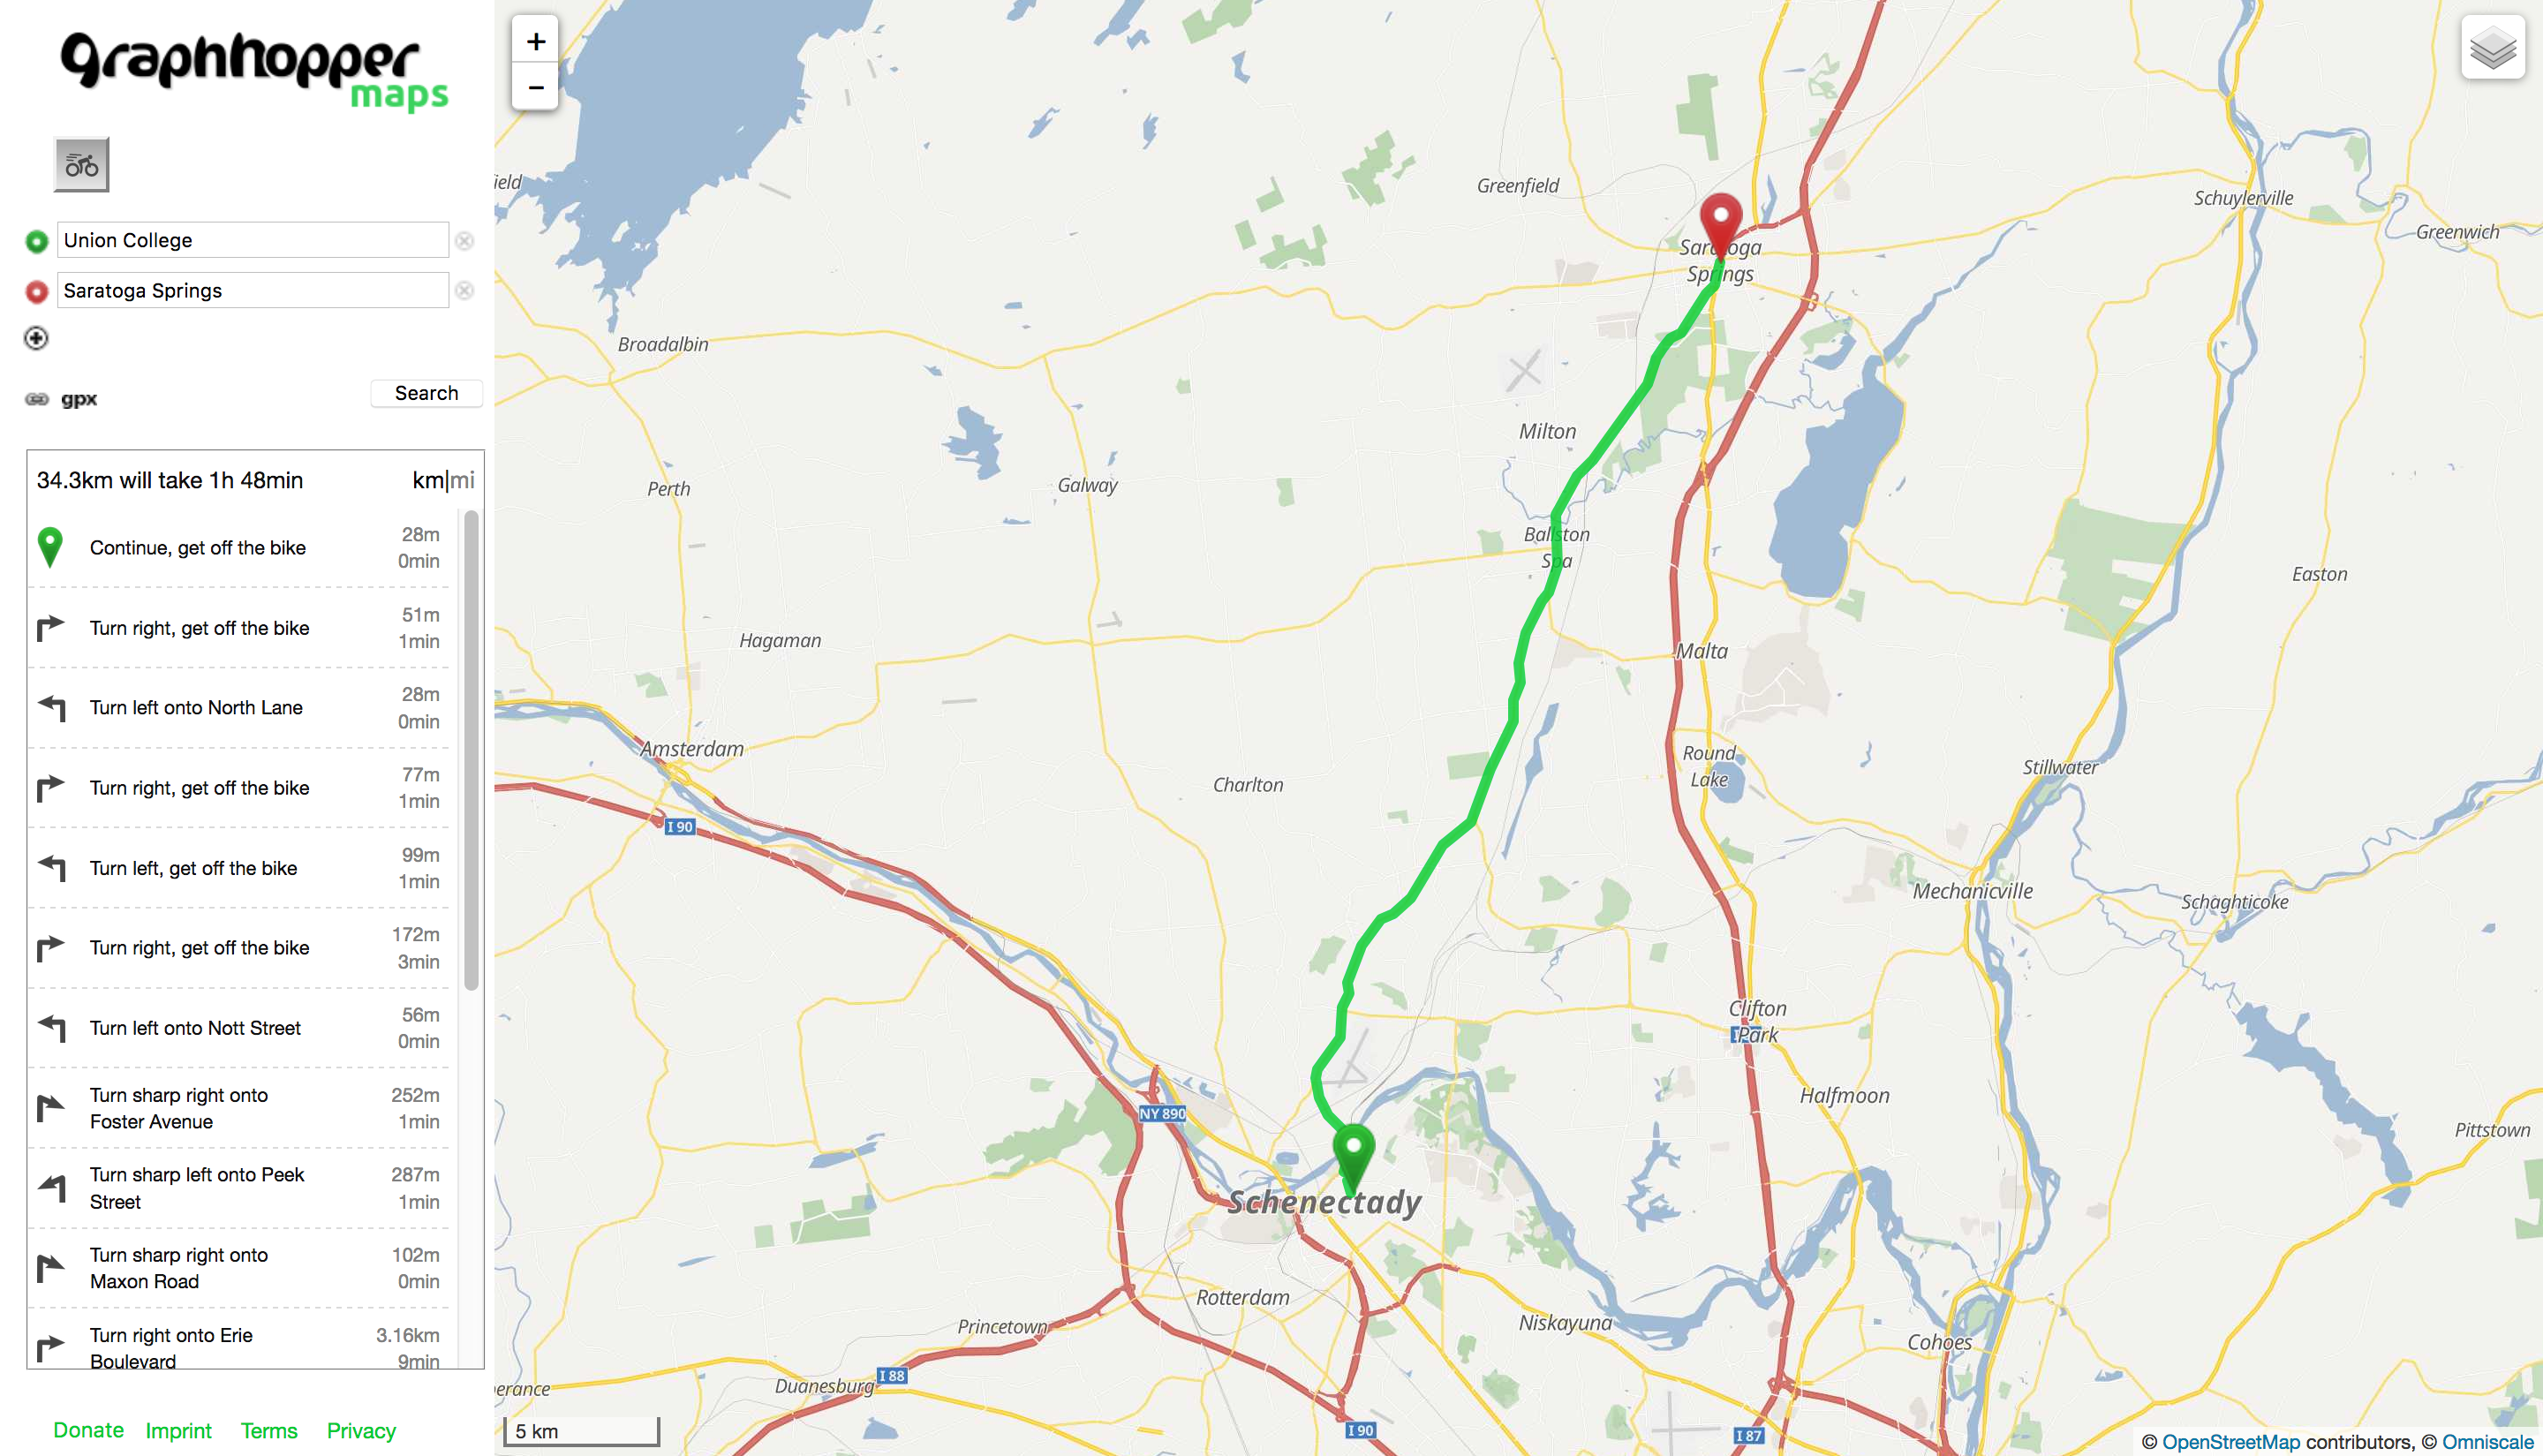
\includegraphics[width=\textwidth]{figs/graphhopper}
    \end{center}
    \caption{GraphHopper web frontend. This is OpenStreetMap data overlaid with the shortest path from Union College to Saratoga Springs.}
    \label{tab:graphhopper-frontend}
\end{figure}

Additionally, GraphHopper supports multiple ``routing profiles" which modify the weights of roads based on a particular vehicle. This is used to give preference to certain roads that are more suited for a particular vehicle. GraphHopper's default bike routing profile contains code for giving the normalized ``priority" value of a road. A normalized priority value is one of the 7 values contained in \cref{tab:osm-hint} normalized to a 0 to 1 scale with 1 being more preferable. When determining the priority of a road, this routing profile also considers other road metadata such as road speed and road surface. We use this normalized priority value calculated by GraphHopper as our road scoring mechanism. A road's cost is simply its distance in meters.


\subsubsection{Contraction Hierarchies}
GraphHopper supports a special type of graph preprocessing called contraction hierarchies \cite{graphhopper}. The goal of contraction hierarchies is to preprocess the graph such that subsequent shortest path queries can be computed more quickly but still provably correct. This is done by ordering nodes by some importance value and then iteratively ``contracting" the least important node. Contracting a node $v$ means replacing shortest paths through $v$ with new shortcut edges \cite{geisberger2008contraction}. A faster shortest path search can be obtained by running a bidirectional shortest-path search making sure that the forward direction only traverses edges going to more important nodes and the backward direction only traverses edges coming from more important nodes.

When running the GraphHopper server for the first time, the engine processes the raw OSM data into a graph and builds contraction hierarchies for each of the enabled routing profiles. This contraction step may take many minutes depending on the size of the graph. We use GraphHopper's built-in contraction hierarchy based shortest path algorithm\footnote{GraphHopper's default algorithm is bidirectional Dijkstra's algorithm.} for calculating shortest paths in both our VVA implementation LS implementation.

\subsection{VVA Implementation}
Our Java implementation of the VVA algorithm differs very little from the pseudocode provided by \citeauthor{verbeeck2014extension} Our implementation does not have a set of starting locations nor does it retain the four best initial solutions. Rather, the starting location is fixed and only the single highest scoring solution is retained between iterations. These choices both simplify our implementation and make the ILS closer to that of the LS algorithm. Our local search heuristic is still a recursive DFS with a maximum depth parameter that performs arc feasibility checking.

Another difference in our implementation is how we check arc feasibility. Instead of precomputing all-pairs shortest path, we use GraphHopper's built in contraction hierarchies and do an online shortest-path computation. This is slower than assuming all shortest paths have been pre-computed and using a lookup table. However, this requires far less computation before the algorithm runs. In addition, we can leverage GraphHopper's fast and correctly implemented shortest-path algorithms without writing our own pre-processing code. Since we are routing on a contraction hierarchy graph, we need to make sure to ignore the special ``shortcut" edges added in the contraction phase. Our road scoring mechanism is GraphHopper's normalized priority value and road costs are distances in meters.

\begin{figure}
    \begin{center}
        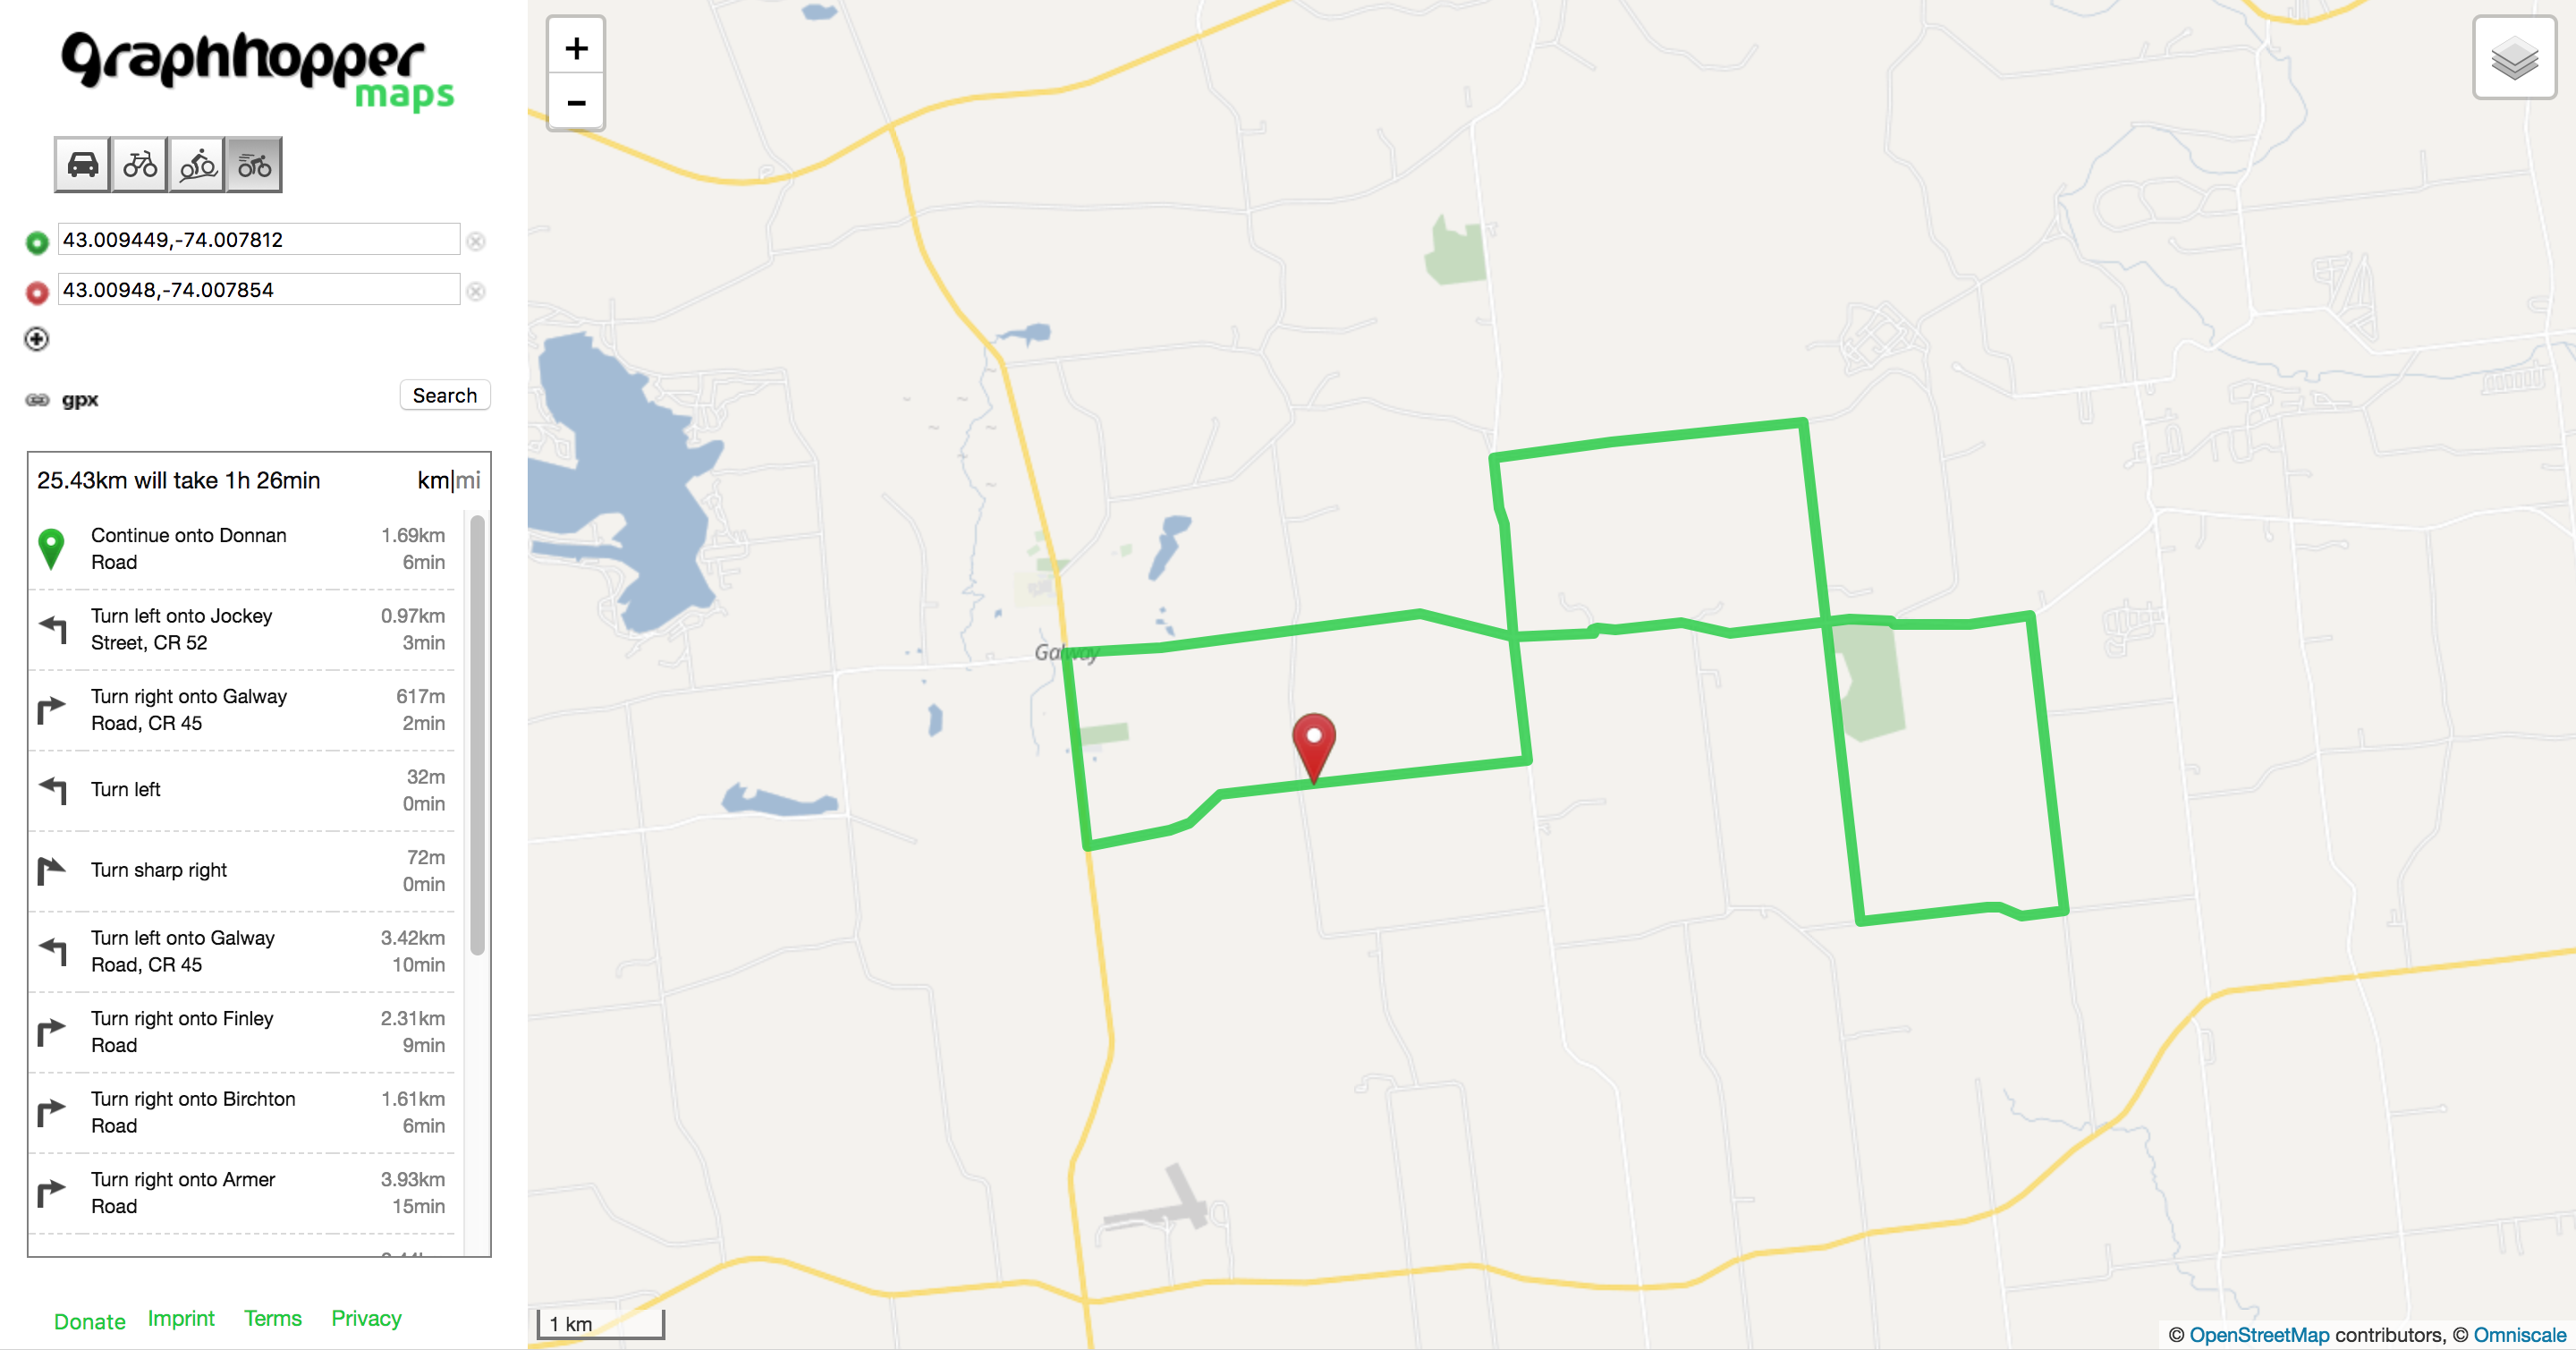
\includegraphics[width=\textwidth]{figs/vva-route}
    \end{center}
    \caption{Example route produced by our implementation of the VVA algorithm.}
    \label{fig:vva-example}
\end{figure}

\begin{figure}
    \begin{center}
        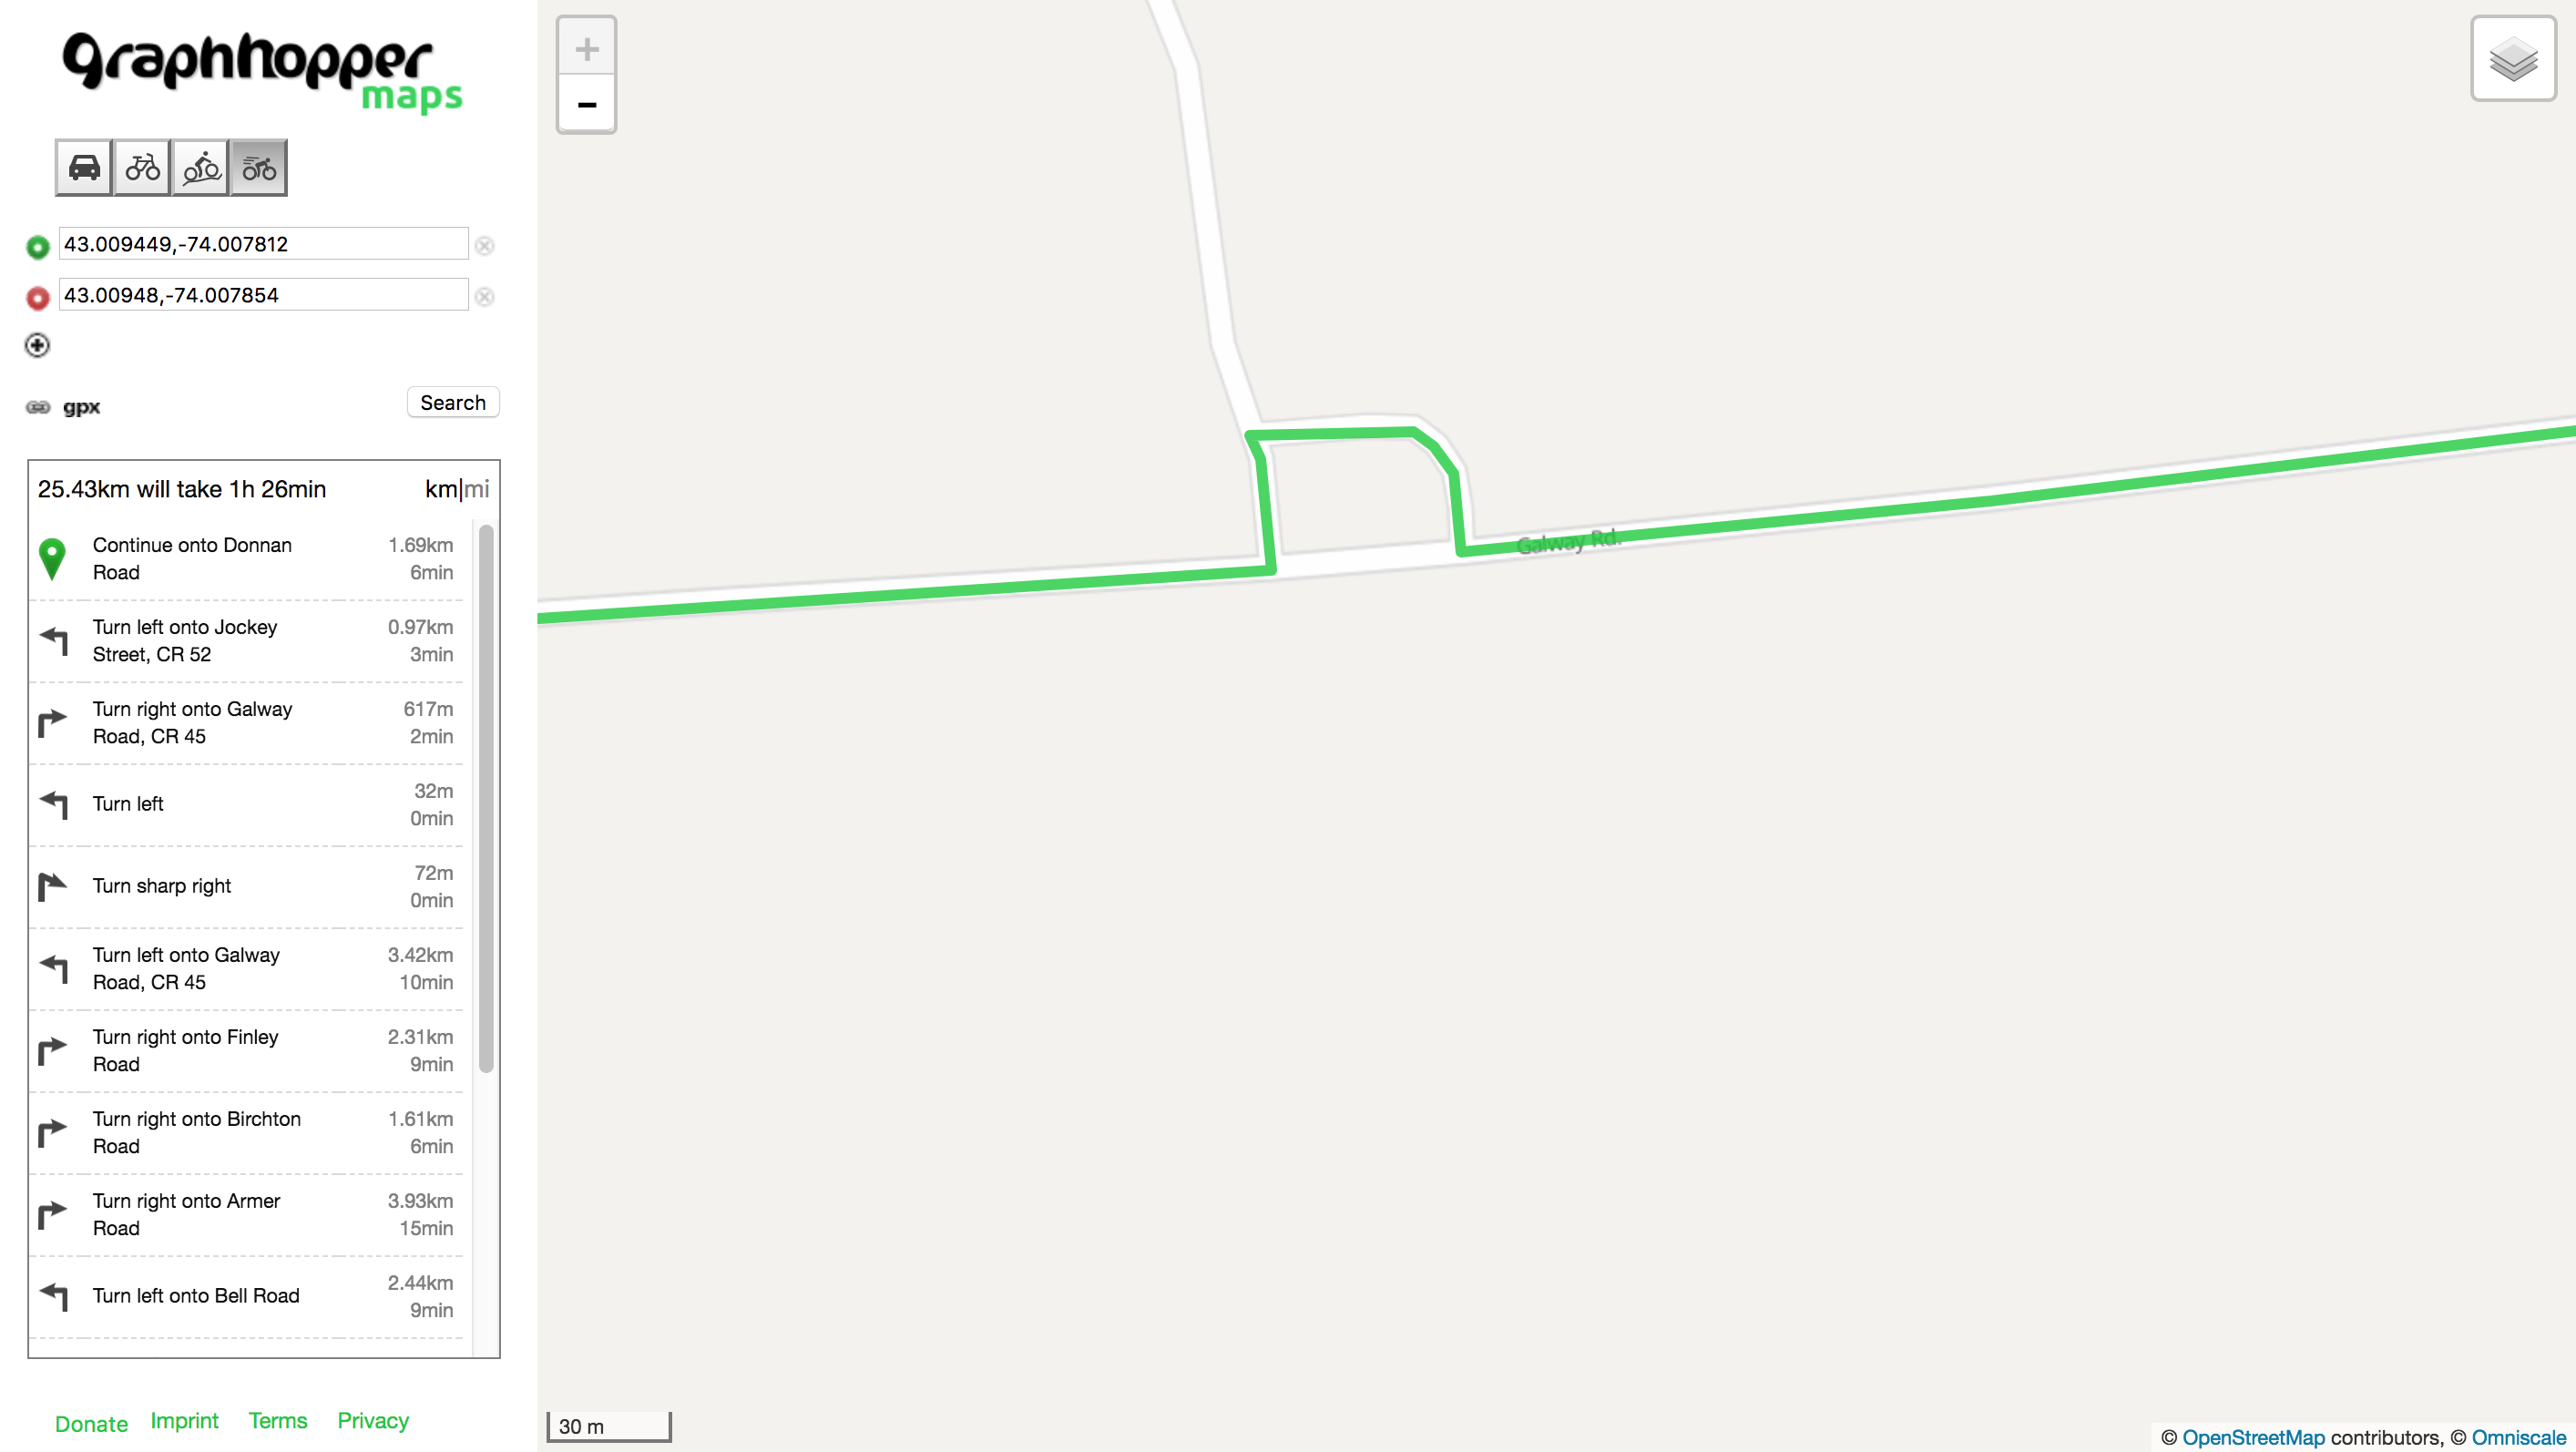
\includegraphics[width=\textwidth]{figs/vva-route-turn}
    \end{center}
    \caption{Quick turns in VVA example route. Inset in \cref{fig:vva-example}}
    \label{fig:vva-example-turn}
\end{figure}


\subsection{LS Implementation}
Compared to the the VVA algorithm, the LS algorithm is more complex so our implementation differs more from the pseudocode provided by \citeauthor{lu2015arc}. There are many more implementation choices to be made. Recall that this algorithm works by connecting together attractive arcs with shortest paths known as ``blank path segments." 

Implicitly defined in the LS algorithm is an object which represents the solution built up through iterations. We call this object a ``Route" and provide a unified interface for adding and removing arcs from this path. When adding and removing arcs, internally the object maintains the blank path segment invariant by calculating shortest paths and storing these paths. When it is time to return the actual path to GraphHopper, the Route object simply iterates over stored attractive arcs and shortest paths (blank path segments) in the correct order. Since we are using a contraction hierarchy shortest path algorithm to compute the blank path segments, we recursively ``unpack" any shortcuts (to get the original roads) before returning the solution to GraphHopper. 

Our Candidate Arc Set (CAS) computation also differs in the way we spatially fetch arcs. We do not use a grid index and fetch all arcs whose grids overlap with the pruning ellipse.  Instead, we perform a breath first search starting at our start node only continuing our search outward if a given road is inside of our pruning ellipse. When the search returns, we have a list of all arcs that are contained solely inside of the pruning ellipse. We compute CAS feasibility of these arcs using the same contraction hierarchy shortest path algorithm used to calculate blank path segments. Our scores and costs are identical to those used in our VVA implementation.


\subsubsection{Implementation Observations}
\label{sec:ls-observations}
Because the LS algorithm is randomized, running the same query multiple times produces different routes. \cref{fig:ls-route1} shows a perfectly circular route. However, a route with these characteristics is not always generated by the algorithm. Running the same query may produce a route such as \cref{fig:ls-route2}. The route in \cref{fig:ls-route2} contains two subpaths which extend outward and return on the same path like cul-de-sacs. In the most extreme case, shown in \cref{fig:ls-route3}, the route is solely composed of these ``backtracking" subpaths. This results from the LS algorithm because attractive arc are being glued together by shortest paths; The shortest path back after taking an attractive arc may be the same path taken to get to the arc's start.

This backtracking shown in \cref{fig:ls-routes} may be undesirable for cyclists. While riding on the same road more than once is not inherently undesirable for recreational cyclists, this may pose a safety issue. Following a route with excess backtracking requires numerous U-turns which can be dangerous for cyclists.  

\begin{figure}
\begin{subfigure}{.48\linewidth}
\centering
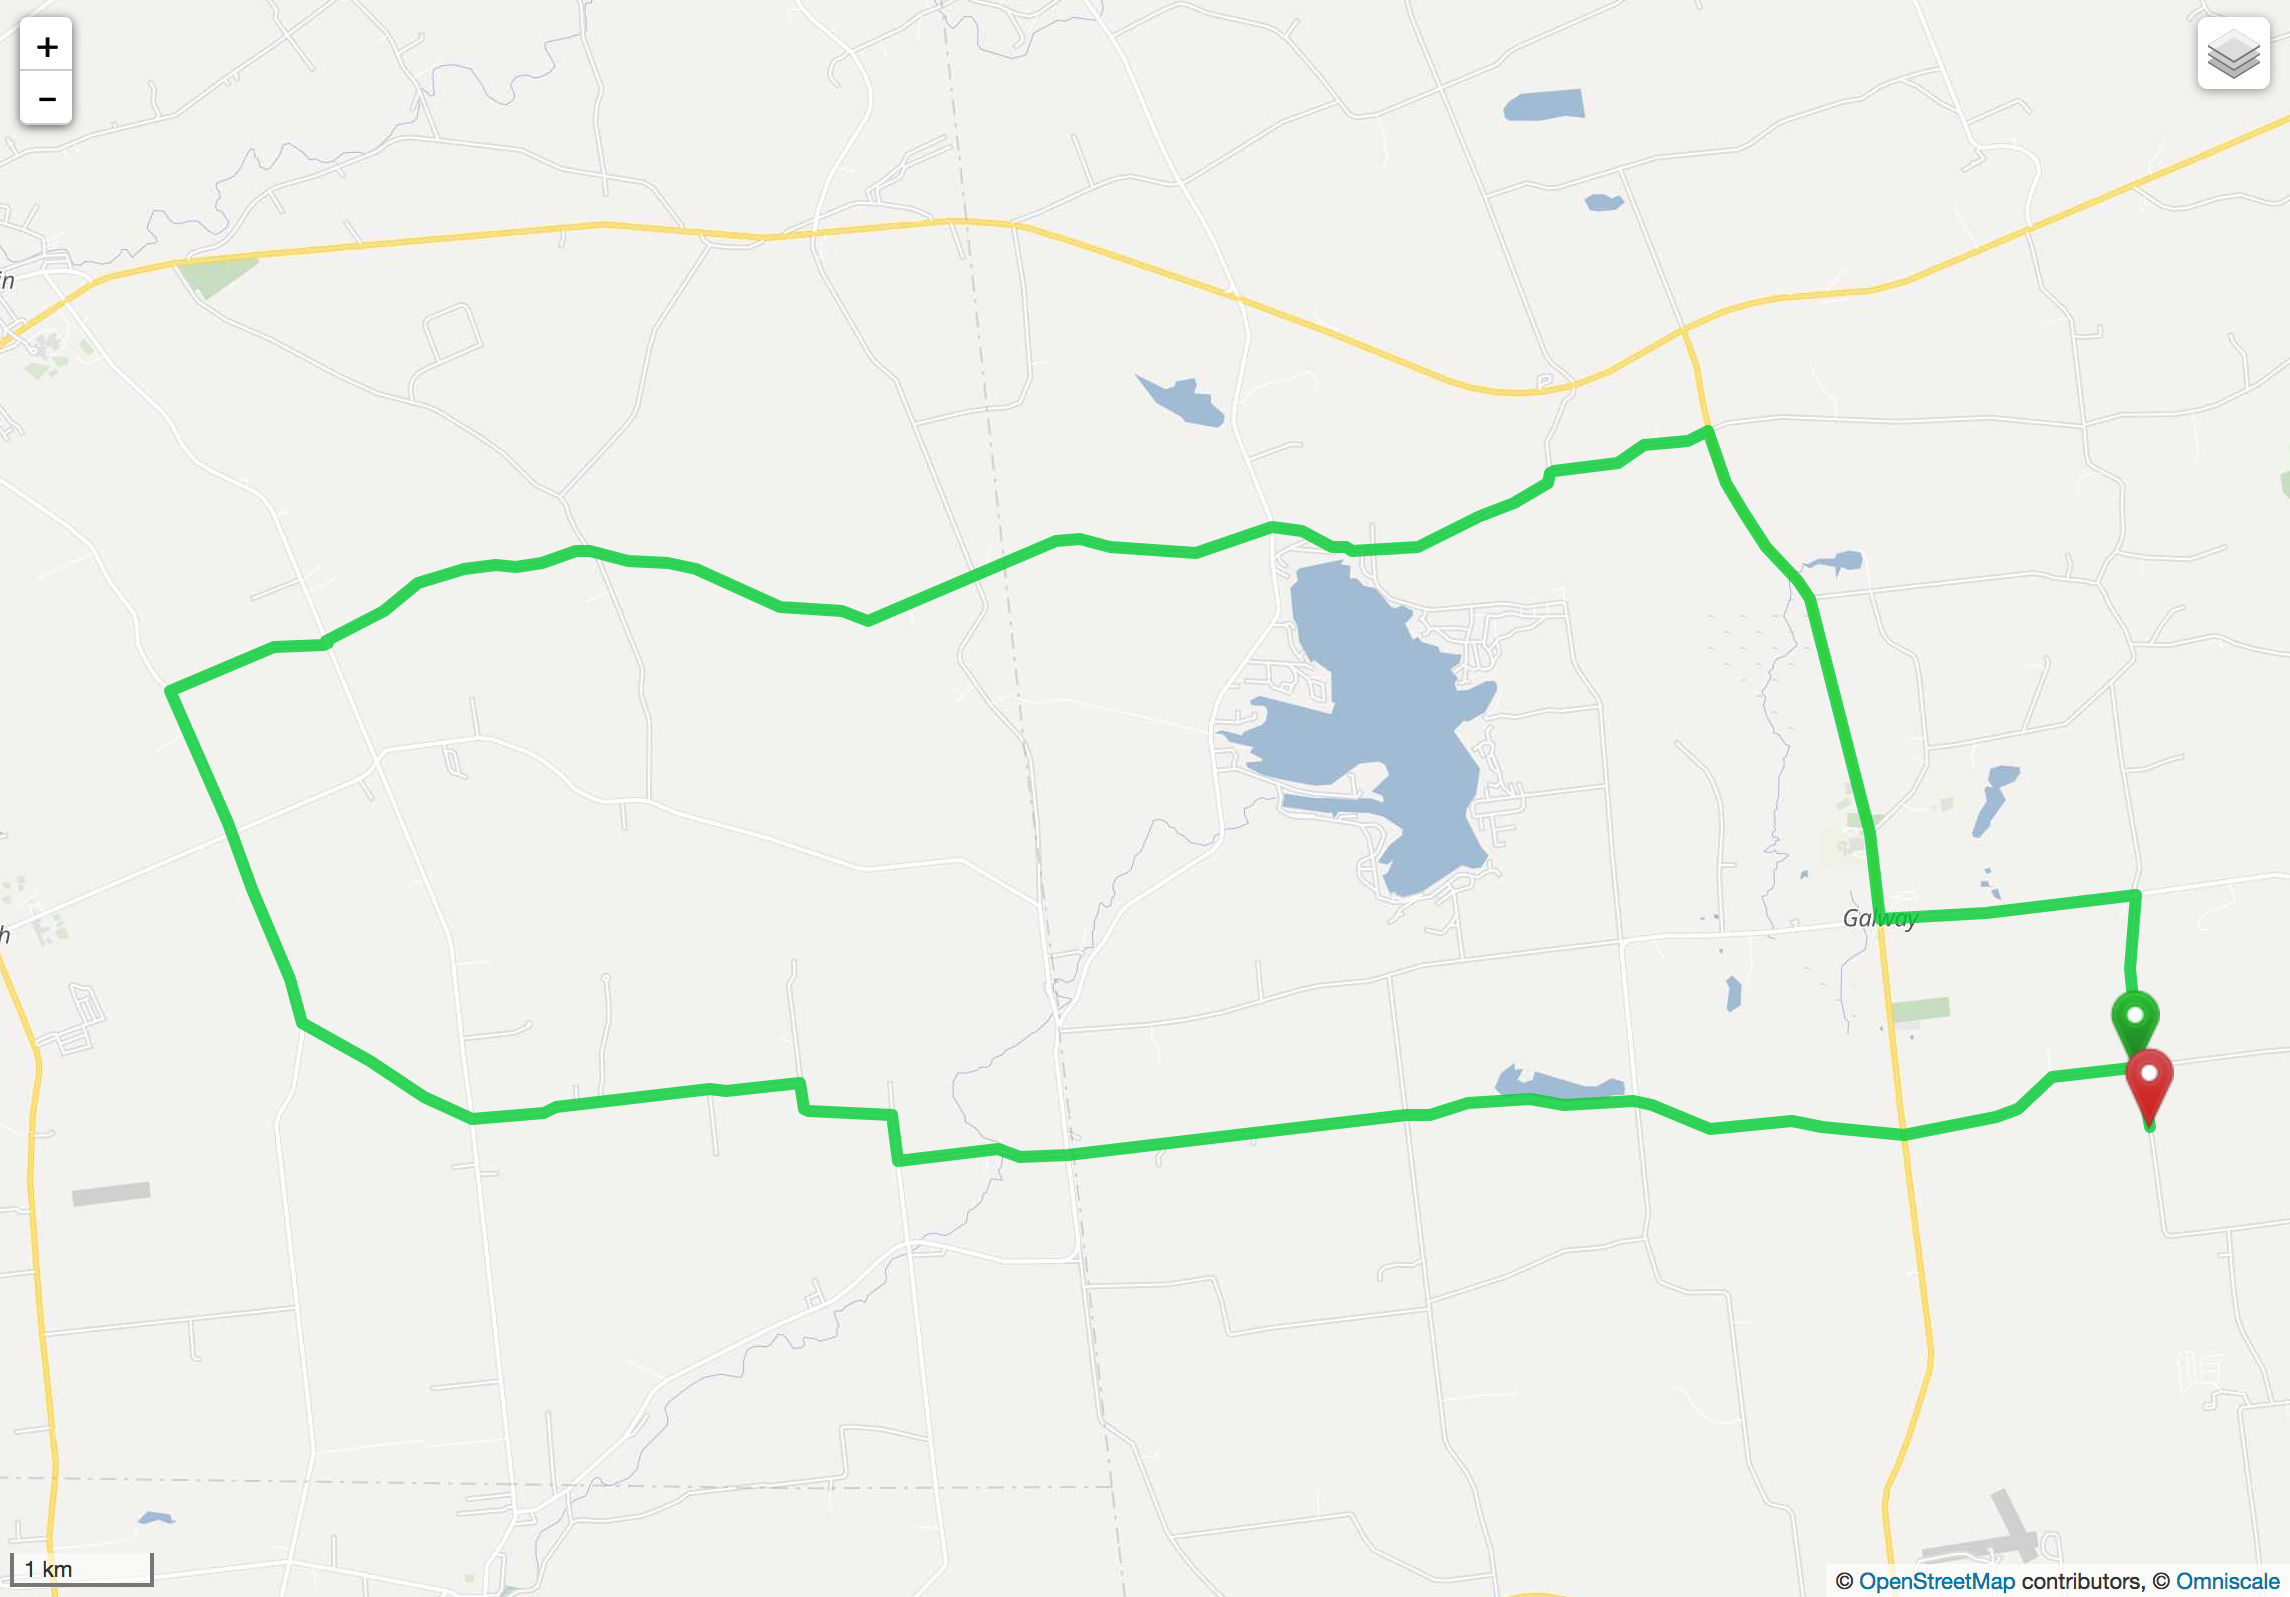
\includegraphics[width=\textwidth]{figs/ls-route1}
\caption{Perfectly circular route}
\label{fig:ls-route1}
\end{subfigure}%
\hfill
\begin{subfigure}{.48\linewidth}
\centering
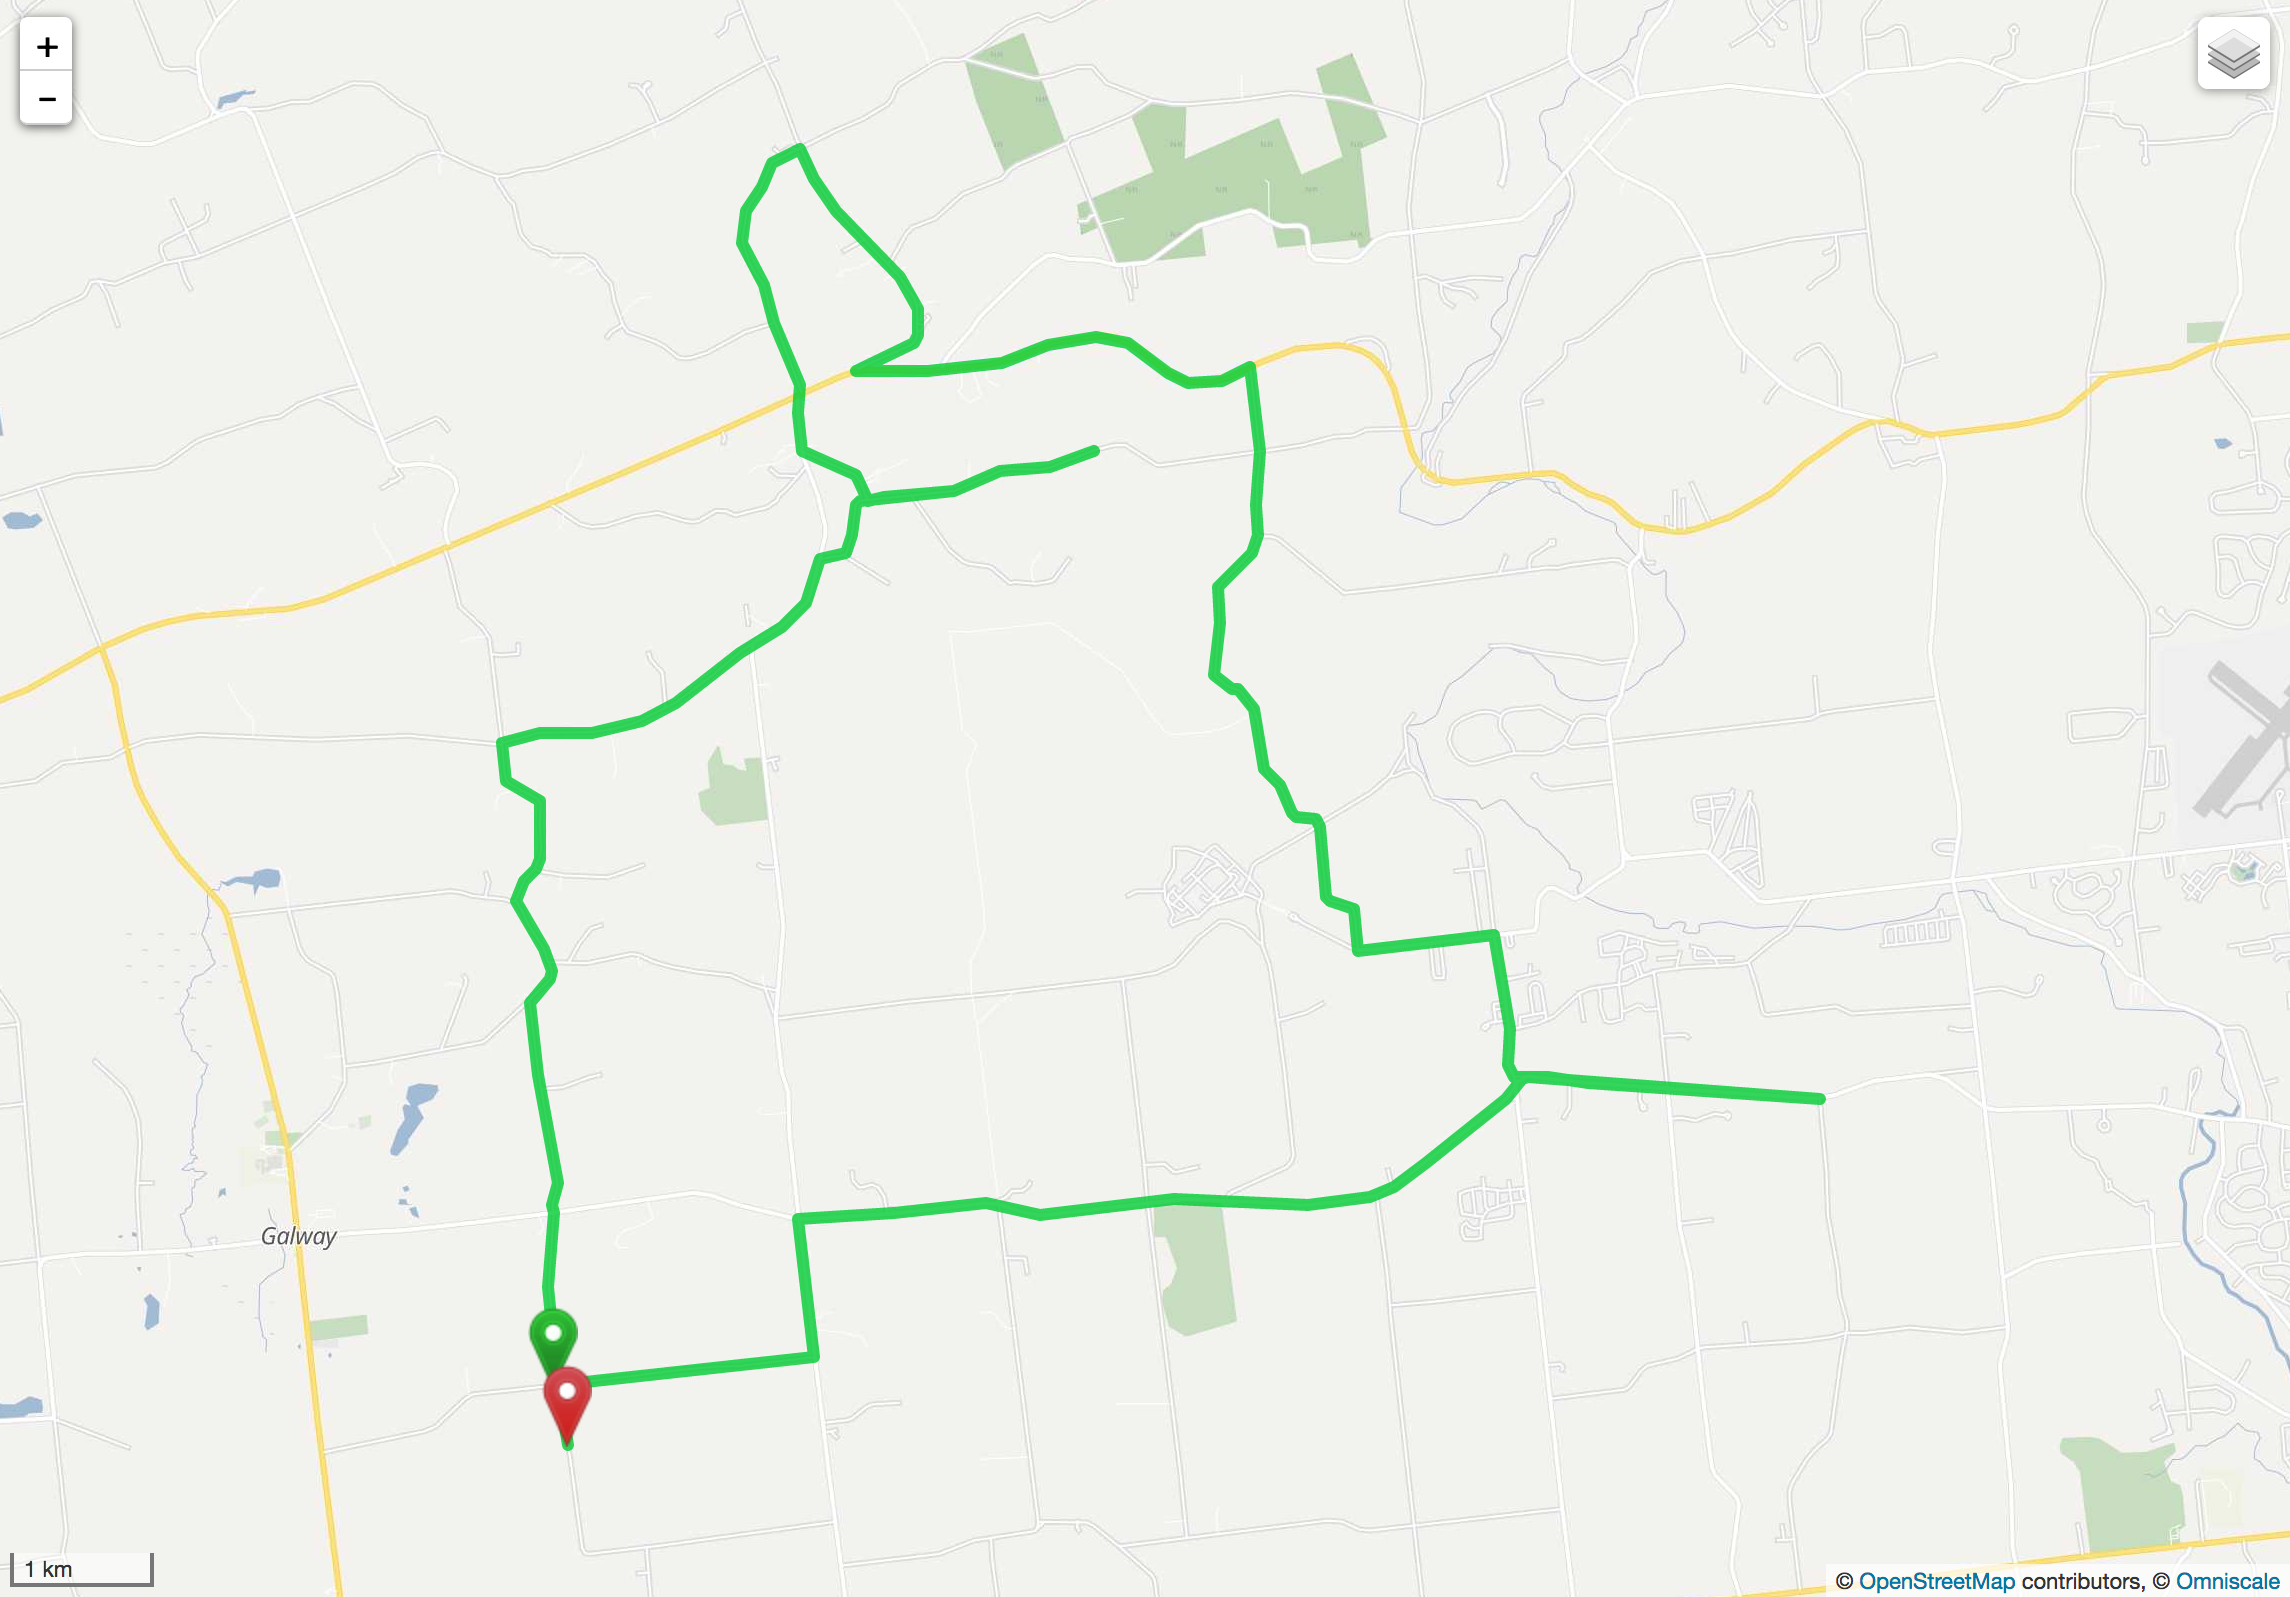
\includegraphics[width=\textwidth]{figs/ls-route2}
\caption{Route with some backtracking}
\label{fig:ls-route2}
\end{subfigure}\\[1ex]
\begin{center}
\begin{subfigure}{0.48\linewidth}
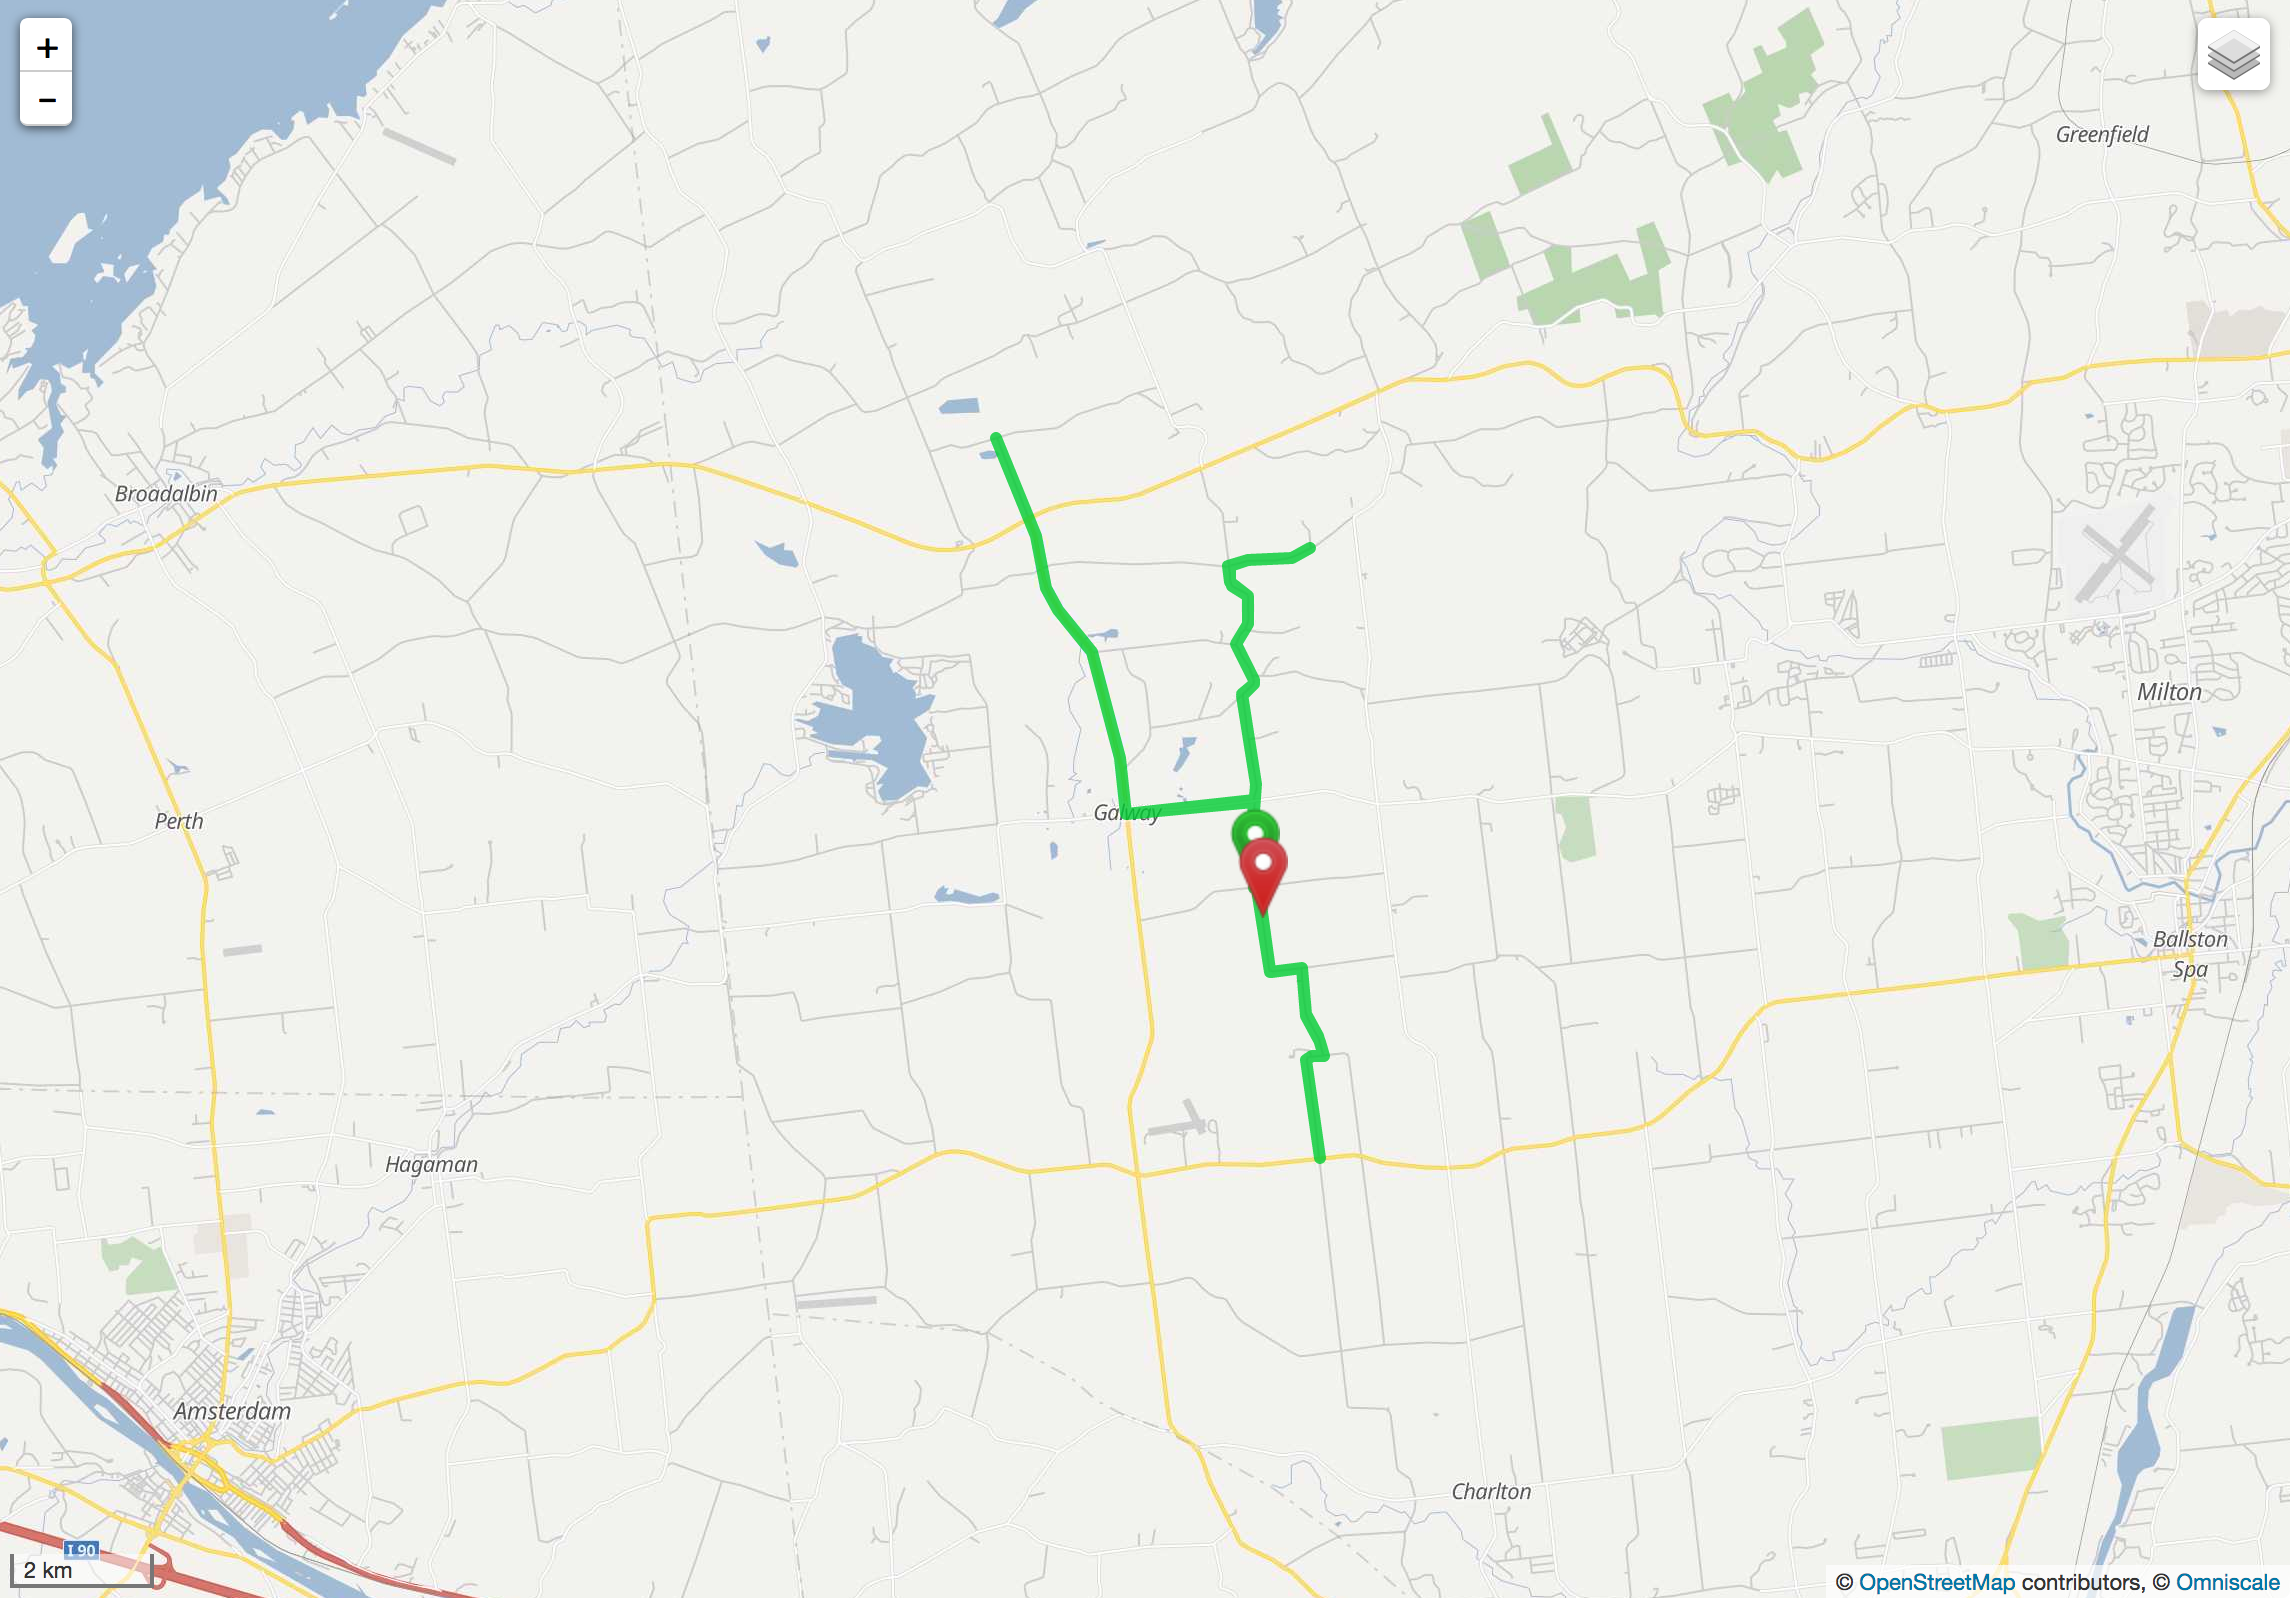
\includegraphics[width=\textwidth]{figs/ls-route3}
\caption{Route with excess backtracking}
\label{fig:ls-route3}
\end{subfigure}
\end{center}
\caption{Example routes generated by our LS implementation with GraphHopper.}
\label{fig:ls-routes}
\end{figure}

Our research implementing the LS algorithm in GraphHopper lead us to the following observations about the algorithm:
\begin{enumerate}
    \item LS does not avoid backtracking when creating blank path segments or when computing arc feasibility.
    \item LS tries to get as close to the cost budget as possible.
    \item LS puts very few restrictions on what is considered an attractive arc.
    \item LS does not penalize turns.
\end{enumerate}

\subsection{Our LS Variants}
We introduce a few variants of LS to address the observations explained in \cref{sec:ls-observations}.

\subsubsection{Budget Allowance}
The LS local search algorithm makes the greedy choice to insert a candidate arc at the smallest blank path segment in the route. This function continuously inserts candidate arcs until the CAS is empty or the cost budget is exhausted. This means that the path returned by \cref{alg:ils-lu-genpath} will normally be very close to the maximum cost. 

The intuition is if the initial route generated by \cref{alg:ils-lu-genpath} is very close to the budget, then there may not be enough budget remaining to make big changes to the route. Therefore, the ILS may get stuck in a local optimum. The ``budget allowance" variant aims to solve this by leaving more budget for later iterations of the search. Given a fixed percentage $0 < p < 1$, this variant ensures that Algorithm 6 is only allowed to use $p \cdot RemainingBudget$ when constructing the path at any given iteration. 

\subsubsection{Incremental Budget}
The ``incremental budget" variant is similar to the ``budget allowance" variant and aims to solve the same problem. However, instead of using a fixed budget percentage, it has a minimum budget percentage $p_{min}$. Over the course of the ILS iterations, the allowed budget scales from $p_{min}$ to $1$ in increments of $(1 - p_{min}) / iterations$. The intuition is that while we want to save budget for later iterations, we shouldn't heavily restrict the budget as we near the termination of the ILS.

\subsubsection{Arc Restrictions}
This variant changes how arcs are chosen to be included in a CAS. In the baseline LS implementation, attractive arcs are arcs whose score is greater than zero. This variant takes in two parameters $minRoadLength$ and $minRoadScore$. An arc is only considered attractive and added to the CAS if its distance in meters is greater than $minRoadLength$ and its score is greater than $minRoadScore$. The intuition behind these restrictions is that the algorithm should not route to an attractive arc that is very small and have a meager score. Similarly, for a particular arc, the distance spent to traverse it should be worthwhile and this is generally true of longer arcs with higher scores. 

\subsubsection{No Backtracking}
This variant attempts to solve the issue displayed in \cref{fig:ls-routes} by ``blacklisting" roads from the shortest path computations. As the algorithm builds up intermediate solutions, we keep track of all the arcs currently in the solution using a HashSet. When it is time to calculate a blank path segment to an attractive arc, we restrict which arcs are allowed to be traversed by the shortest path algorithm using the HashSet and the attractive arc. When calculating the blank path segment away from the attractive arc, we need to blacklist not only the roads in the solution but the roads in the first blank path segment as well. This practice has two key implementation details which we address.

First, blacklisting roads may break the shortest path computation. In a connected graph there is always some shortest path between any two nodes. However, if we restrict which roads are allowed in the search then it is possible that we may have no shortest path. For example, consider an attractive arc at the end of a dead end road. Computing the first blank path segment to the arc will succeed but we cannot take the same path back so we have no return segment. In the case where we have no available blank path segment, we set the total path cost to \emph{infinity}. This means that the arc will no longer be included in the CAS since it cannot feasibly update any arcs. 

Second, this blacklisting process does not work well with contraction hierarchies. Recall that a contraction-hierarchy shortest-path algorithm traverses over contracted ``shortcut" edges in the graph. The actual returned shortest path is recreated by finding the original roads which these shortcuts skip over. When determining if a road is blacklisted in our shortest path traversal, we need to check whether our current road is a shortcut and if it is, make sure none of the roads it skips are also blacklisted. This is quite challenging since a shortcut may skip multiple roads and may skip other shortcut edges. This means that we need to recursively ``unpack" a shortcut (and any skipped shortcuts)  before we can determine if we should avoid the arc. This is effectively undoing all the pre-computation that is done when the contraction hierarchy is initialized. In order to avoid this problem, our no-backtracking variant does not use a contraction hierarchy shortest-path algorithm.


\section{Data}
\label{sec:data}
We ran a series of experiments to evaluate the performance of the VVA algorithm, the LS algorithm, and our LS variants. This section discusses our data set, data collection process, and experimental results.

\subsection{Map Data}
Our mapping data set is a OpenStreetMap file\footnote{In Protocolbuffer Binary Format (.pbf). PBF is an alternative to the XML format which provides better compression.} corresponding to 350 square kilometers centered around Galway, NY. The free online tool \emph{BBBike Extract} \cite{bbbike} was used to obtain the data. When parsed by GraphHopper, the internal graph representation contains 2425 directed arcs and 982 nodes. We chose this dataset because it is relatively small and is moderately road dense. The size of the road network was also chosen to make an Integer Programming evaluation feasible. See \cref{sec:int-programming} for more information on this approach.

\subsection{Data Collection}
We ran 500 trials of each algorithm configuration (\cref{tab:algo-configs}) fixing the start location, the cost budget, and the number of ILS iterations. To achieve circular routes, the start and end location was fixed at GPS position $(43.009327, -74.009166)$, the center of our OSM data set. The cost budget was fixed at 40 kilometers. The number of iterations was fixed at 100. Our experiments use unit scoring. Thus, if two roads of different length have the same priority value by GraphHopper then they have the same score which is its priority value directly. These choices are mostly arbitrary. The iteration number and cost budget were chosen to be similar to the experimental tests run by \citeauthor{verbeeck2014extension} and \citeauthor{lu2015arc}.

The ILS algorithms were modified to record the current solution score and elapsed time at each iteration. These values were written to a single CSV file for each algorithm configuration. For each configuration, average scores and average times were calculated using pivot tables with Python and Pandas\footnote{A Python package for data manipulation and analysis.}. The experimental runs were performed on a computer with 4 Intel Xeon E5620 processors and 16GB of RAM running Ubuntu 16.04.03 LTS Desktop.

\begin{table}
\begin{center}
\begin{tabular}{|l|l|}
\hline
\textbf{Algorithm} & \textbf{Extra Parameters} \\
\hline
VVA & $maxDepth=20$ \\
\hline
LS & N/A \\
\hline
LS + (Budget Allowance) & $p_{min}=0.5$ \\
\hline
LS + (Incremental Budget) & $p_{min}=0.5$ \\
\hline
LS + (Arc Restrictions) & $minRoadLength=1km$, $minRoadScore=0.5$  \\
\hline
LS + (No Backtracking) & N/A \\
\hline
LS + (Budget Allowance) + (Arc Restrictions) & $minRoadLength=1km$, $minRoadScore=0.5$, $p_{min}=0.5$   \\
\hline
\end{tabular}
\end{center}
\caption{Experimental algorithm configurations}
\label{tab:algo-configs}
\end{table}

\section{Experimental Results}
First, we present images of example routes generated by our LS variants (\cref{fig:ls-route-variants}). In \cref{sec:iteration-cutoff} we present our performance data using the iteration number as the cutoff. Lastly, in \cref{sec:score-cutoff} we analyze a more efficient ILS stopping criterion.  

\begin{figure}
\begin{subfigure}{.48\linewidth}
\centering
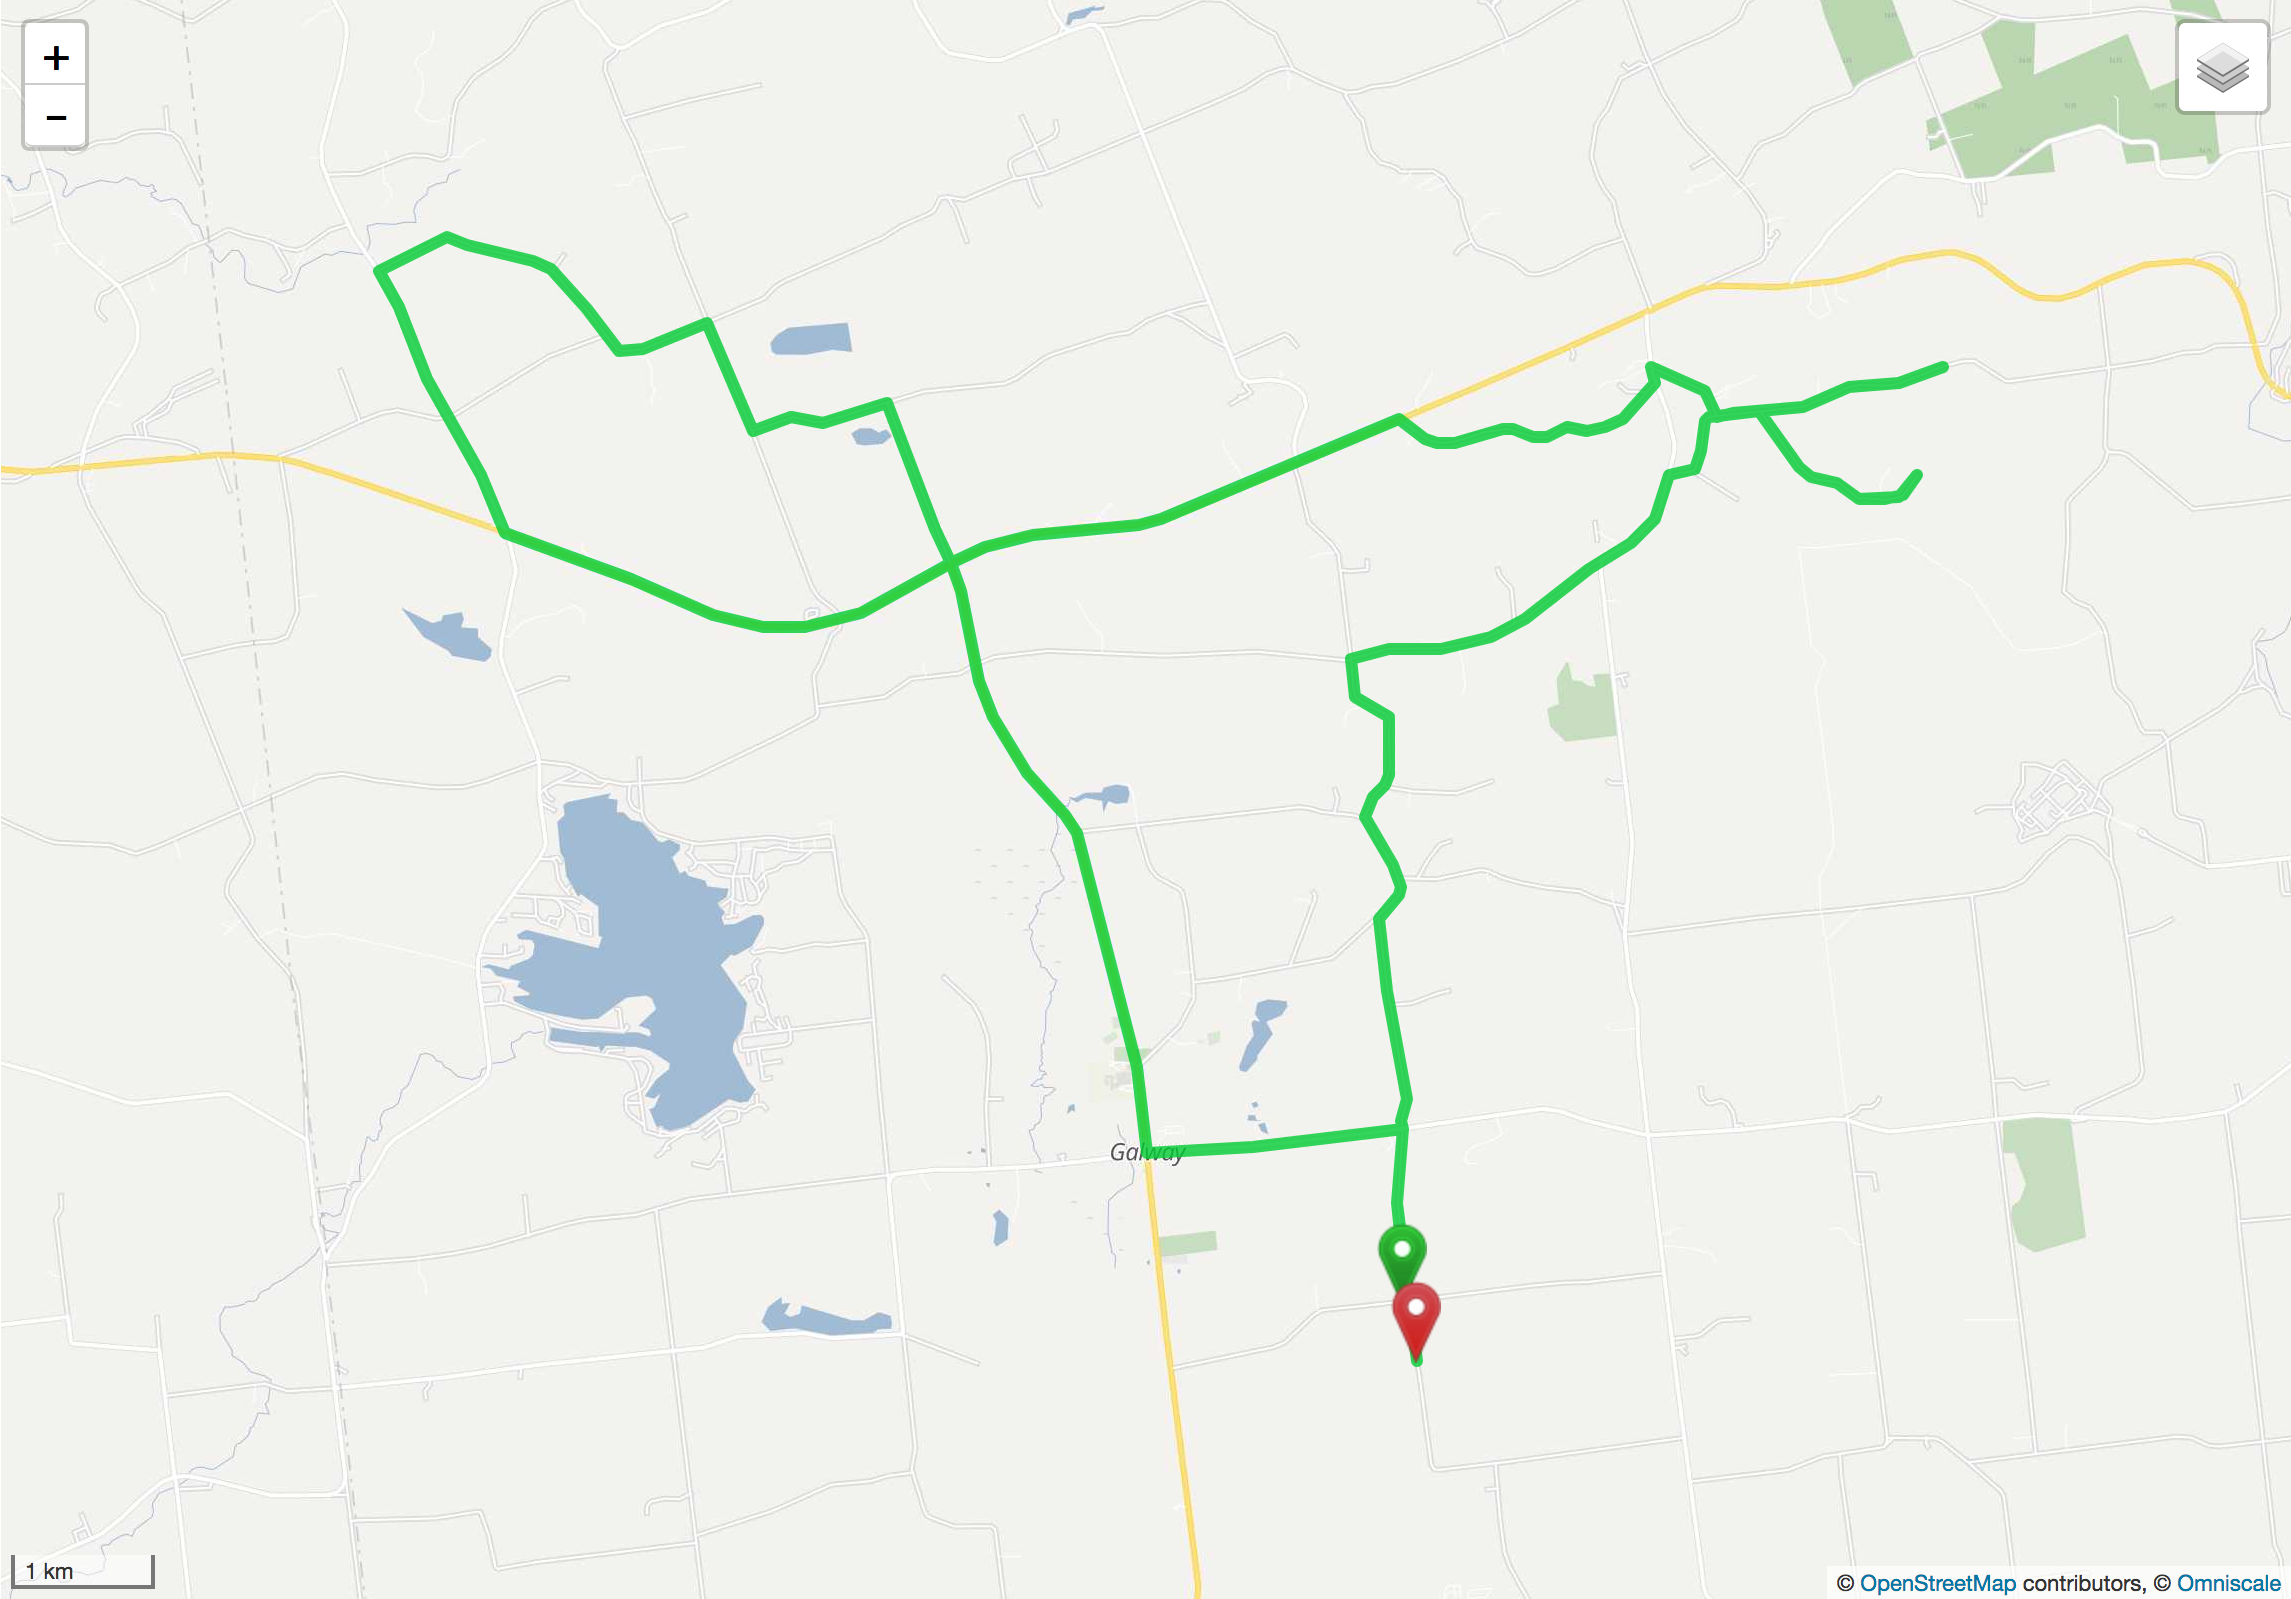
\includegraphics[width=\textwidth]{figs/ls-route-mins}
\caption{Example route generated by LS + (Arc Restrictions)}
\label{fig:ls-arc-restrictions}
\end{subfigure}%
\hfill
\begin{subfigure}{.48\linewidth}
\centering
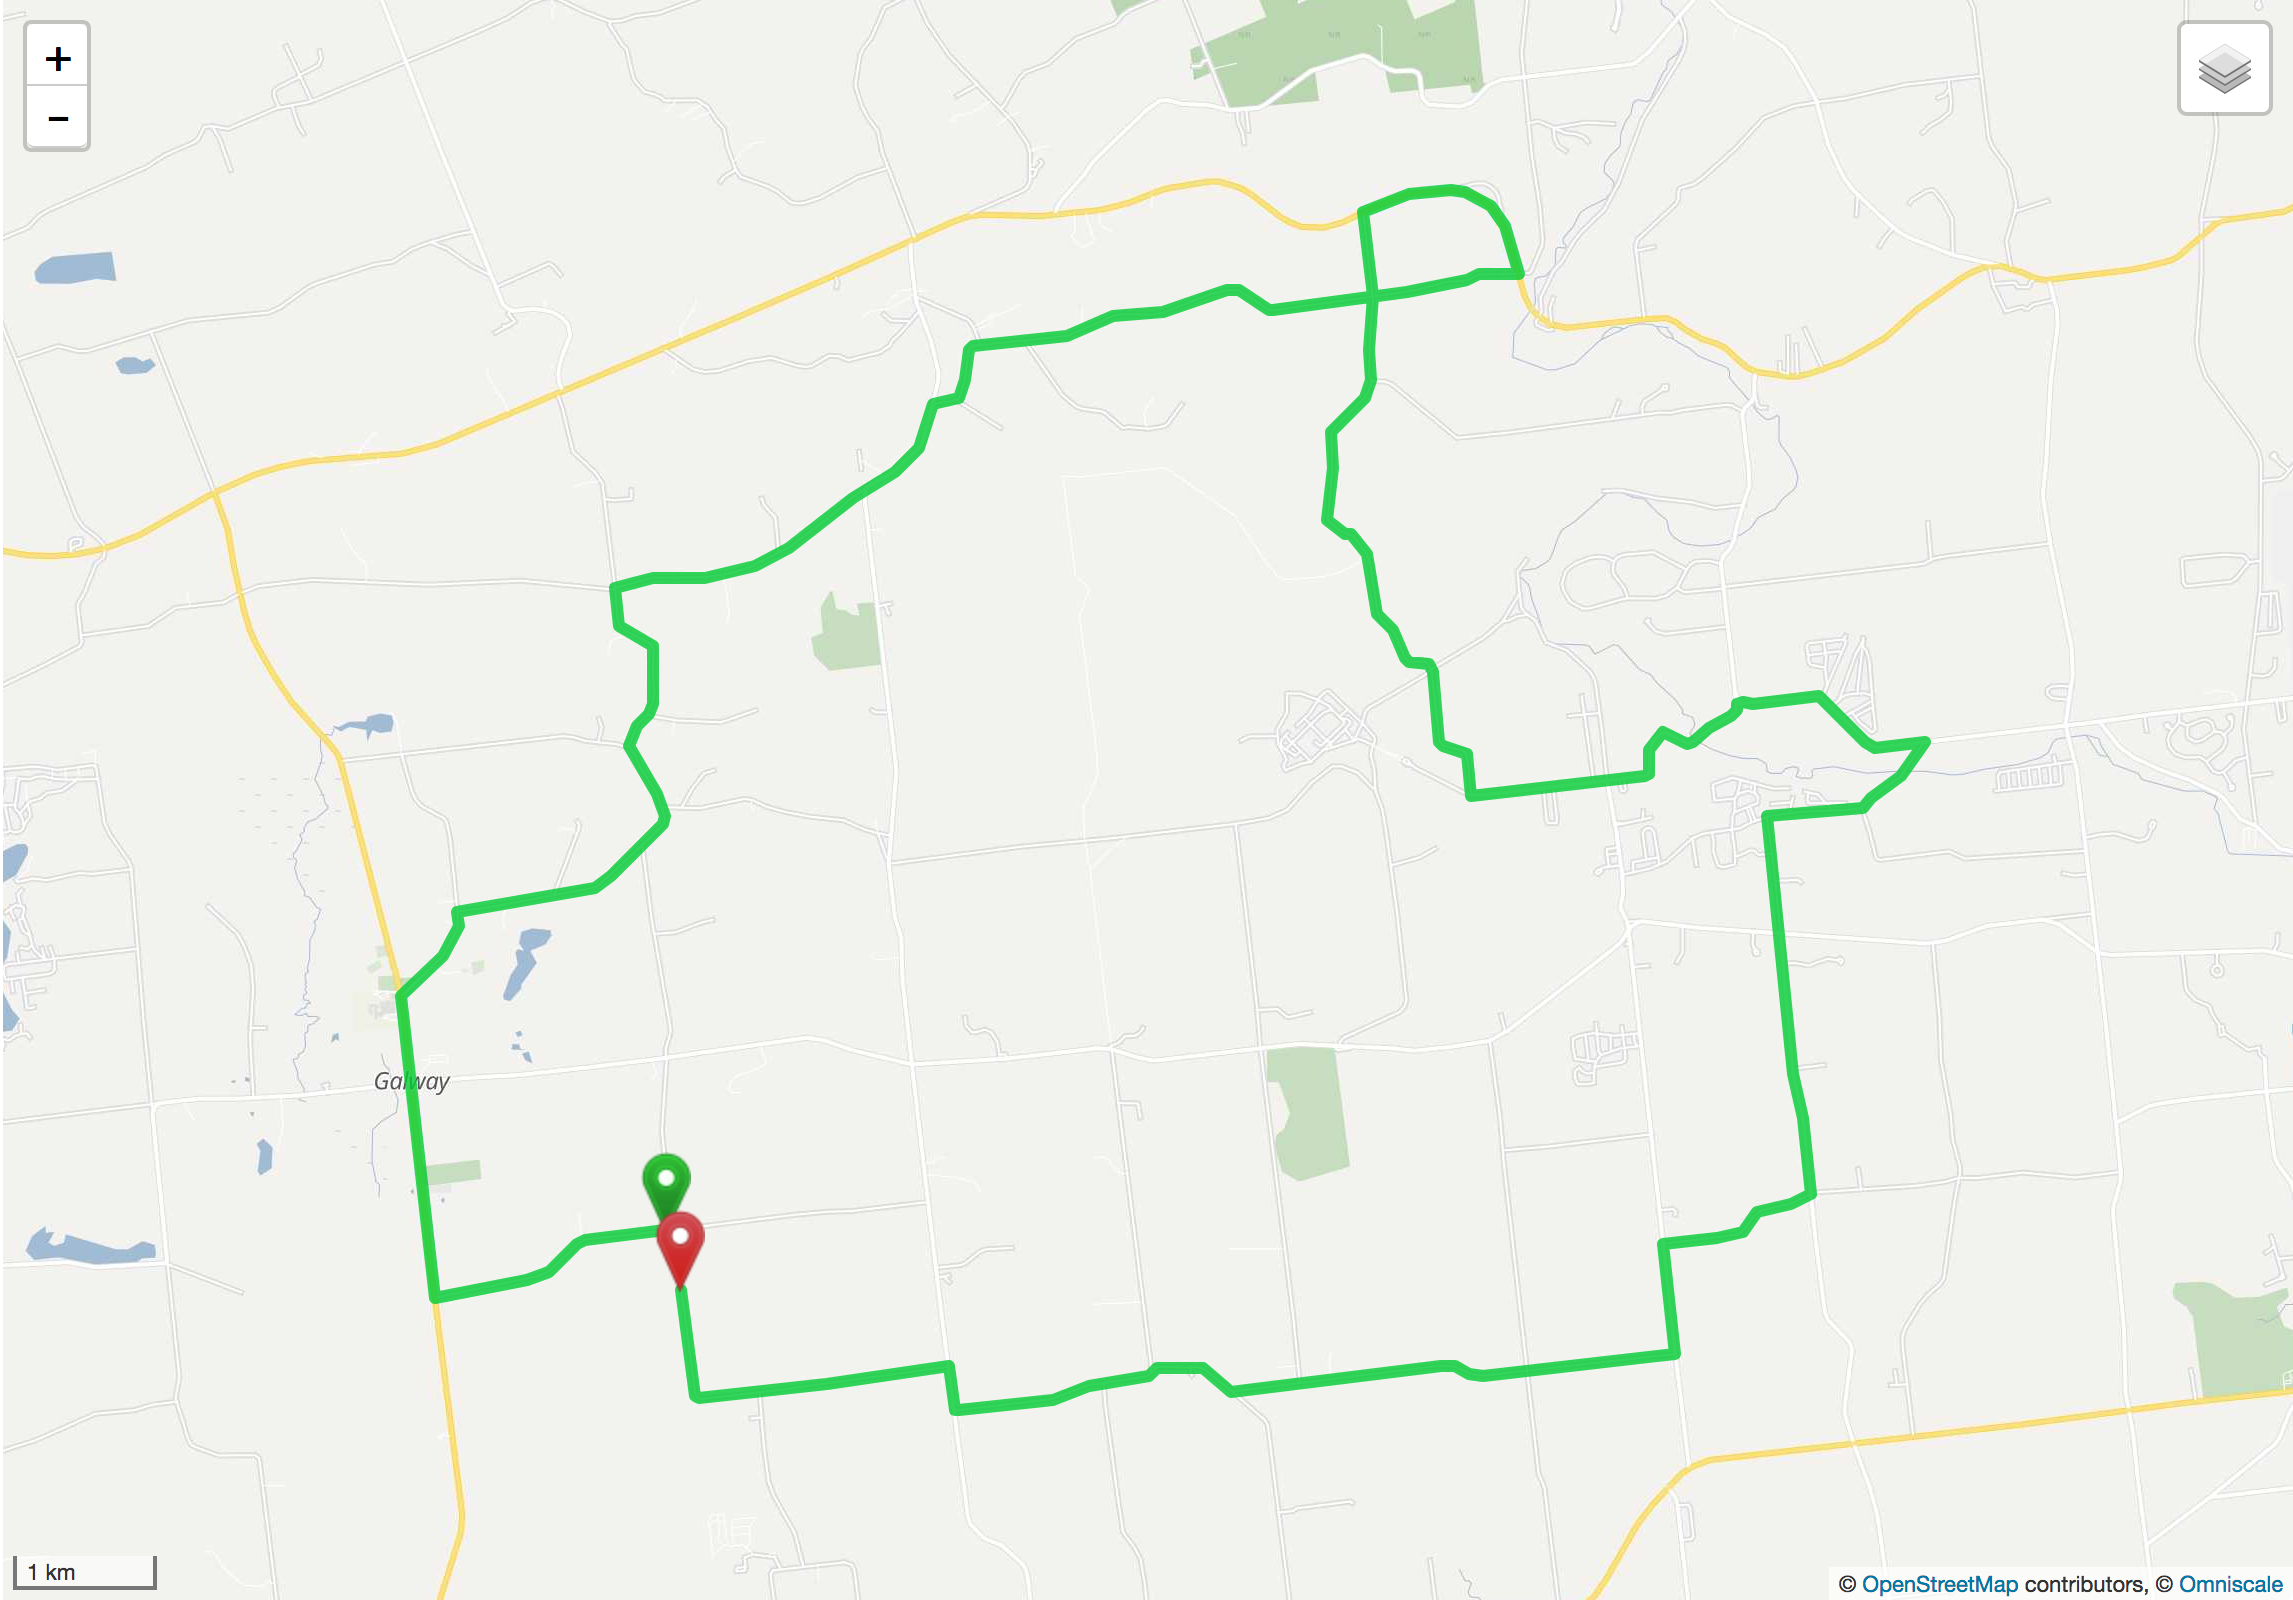
\includegraphics[width=\textwidth]{figs/ls-route-no-backtracking}
\caption{Example route generated by LS + (No Backtracking)}
\label{fig:ls-no-backtracking}
\end{subfigure}\\[1ex]
\caption{Example routes generated by our LS variants implemented with GraphHopper.}
\label{fig:ls-route-variants}
\end{figure}

\subsection{Iteration Cutoff}
\label{sec:iteration-cutoff}
\cref{tab:unit-scoring-results} shows the times and scores of each algorithm configuration after 100 iterations. Independent plots of score and time versus iteration number are shown in \cref{fig:graphs-unit-scoring-ls}. A combined plot of variant score versus iteration number is shown in \cref{fig:graphs-combined-unit-scoring}.

\label{sec:unit-scoring}
\begin{table}
\begin{center}
\begin{tabular}{|l|l|l|l|}
    \hline
    \textbf{Algorithm} & \textbf{Score} & \textbf{Time (s)} & \textbf{Score/Time Ratio} \\
    \hline
    VVA & 20.57 & 20.37 & 1.00 \\
    \hline
    LS & 126.13 & 1.20 & 105.10 \\
    \hline
    LS + (Budget Allowance) & 215.87 & 23.12 & 9.33 \\
    \hline
    LS + (Incremental Budget) & 282.66 & 119.52 & 2.36 \\
    \hline
    LS + (Arc Restrictions) & 49.85 & 0.09 & 553.88 \\
    \hline
    LS + (No Backtracking) & 33.36 & 0.60 & 55.6 \\
    \hline
    LS + (Budget Allowance) + (Arc Restrictions) & 32.49 & 2.37 & 13.70  \\
    \hline
\end{tabular}
\caption{Algorithm performance after 100 iterations with unit scoring.}
\label{tab:unit-scoring-results}
\end{center}
\end{table}

% INDIVIDUAL GRAPHS
\begin{figure}
\begin{subfigure}{.45\linewidth}
\begin{center}
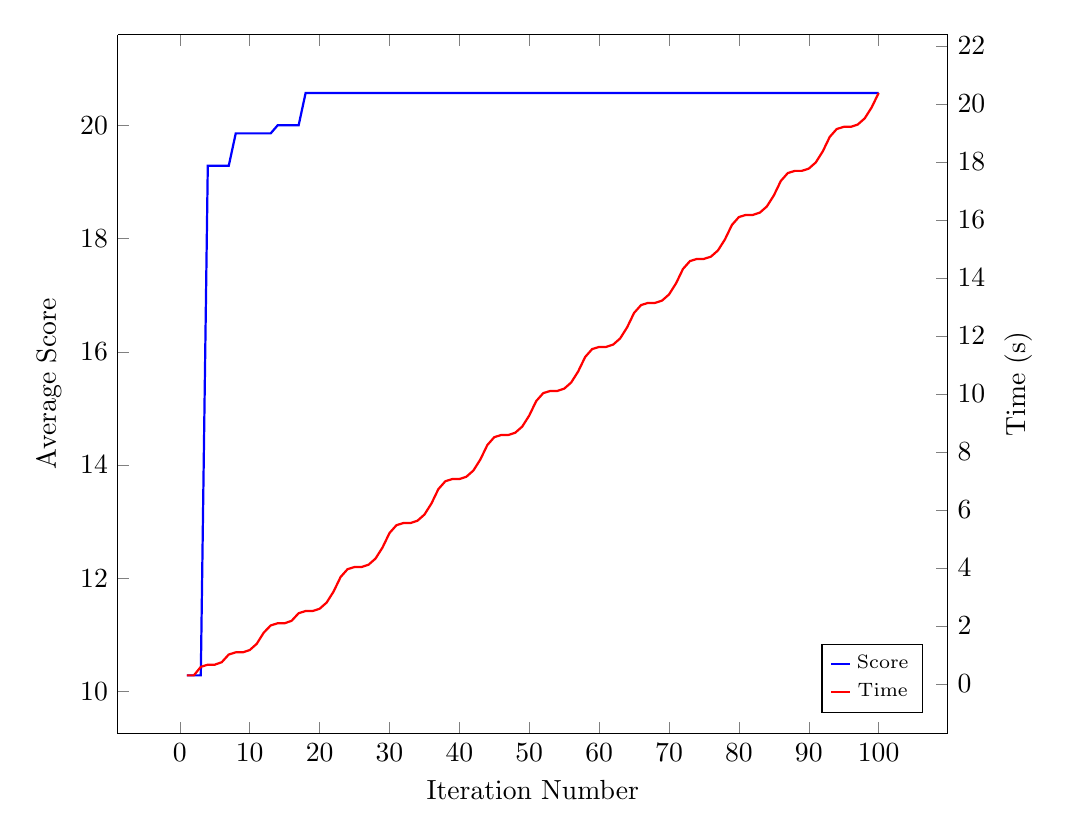
\begin{tikzpicture}
\begin{axis}[
    width=\textwidth,
    xlabel={Iteration Number},
    ylabel={Average Score},
    axis y line* = left,
]
\addplot[
    color=blue,
    style={thick}
    ]
    coordinates {
    (1, 10.285714000000002)(2, 10.285714000000002)(3, 10.285714000000002)(4, 19.285713999999995)(5, 19.285713999999995)(6, 19.285713999999995)(7, 19.285713999999995)(8, 19.857142999999997)(9, 19.857142999999997)(10, 19.857142999999997)(11, 19.857142999999997)(12, 19.857142999999997)(13, 19.857142999999997)(14, 20.0)(15, 20.0)(16, 20.0)(17, 20.0)(18, 20.571429000000002)(19, 20.571429000000002)(20, 20.571429000000002)(21, 20.571429000000002)(22, 20.571429000000002)(23, 20.571429000000002)(24, 20.571429000000002)(25, 20.571429000000002)(26, 20.571429000000002)(27, 20.571429000000002)(28, 20.571429000000002)(29, 20.571429000000002)(30, 20.571429000000002)(31, 20.571429000000002)(32, 20.571429000000002)(33, 20.571429000000002)(34, 20.571429000000002)(35, 20.571429000000002)(36, 20.571429000000002)(37, 20.571429000000002)(38, 20.571429000000002)(39, 20.571429000000002)(40, 20.571429000000002)(41, 20.571429000000002)(42, 20.571429000000002)(43, 20.571429000000002)(44, 20.571429000000002)(45, 20.571429000000002)(46, 20.571429000000002)(47, 20.571429000000002)(48, 20.571429000000002)(49, 20.571429000000002)(50, 20.571429000000002)(51, 20.571429000000002)(52, 20.571429000000002)(53, 20.571429000000002)(54, 20.571429000000002)(55, 20.571429000000002)(56, 20.571429000000002)(57, 20.571429000000002)(58, 20.571429000000002)(59, 20.571429000000002)(60, 20.571429000000002)(61, 20.571429000000002)(62, 20.571429000000002)(63, 20.571429000000002)(64, 20.571429000000002)(65, 20.571429000000002)(66, 20.571429000000002)(67, 20.571429000000002)(68, 20.571429000000002)(69, 20.571429000000002)(70, 20.571429000000002)(71, 20.571429000000002)(72, 20.571429000000002)(73, 20.571429000000002)(74, 20.571429000000002)(75, 20.571429000000002)(76, 20.571429000000002)(77, 20.571429000000002)(78, 20.571429000000002)(79, 20.571429000000002)(80, 20.571429000000002)(81, 20.571429000000002)(82, 20.571429000000002)(83, 20.571429000000002)(84, 20.571429000000002)(85, 20.571429000000002)(86, 20.571429000000002)(87, 20.571429000000002)(88, 20.571429000000002)(89, 20.571429000000002)(90, 20.571429000000002)(91, 20.571429000000002)(92, 20.571429000000002)(93, 20.571429000000002)(94, 20.571429000000002)(95, 20.571429000000002)(96, 20.571429000000002)(97, 20.571429000000002)(98, 20.571429000000002)(99, 20.571429000000002)(100, 20.571429000000002)
    };
\end{axis}

\begin{axis}[
    width=\textwidth,
    ylabel near ticks, yticklabel pos=right,
    ylabel={Time (s)},
    legend pos = {south east},
    legend style={font=\scriptsize\selectfont,},
    legend image post style={scale=0.4},
    hide x axis,
    axis y line*=right,
]
\addlegendimage{/pgfplots/refstyle=vva-graph-score, blue,style=thick}\addlegendentry{Score}
\addplot[
    color=red,
    style={thick}
    ]
    coordinates {
    (1, 0.2917333333333334)(2, 0.29176666666666673)(3, 0.5858)(4, 0.6609333333333333)(5, 0.6610666666666667)(6, 0.7467333333333334)(7, 1.0115666666666667)(8, 1.0864333333333331)(9, 1.0864666666666665)(10, 1.1650333333333334)(11, 1.3789999999999998)(12, 1.7636999999999998)(13, 2.013966666666667)(14, 2.0892)(15, 2.0892333333333335)(16, 2.174633333333333)(17, 2.436166666666667)(18, 2.510466666666667)(19, 2.510666666666667)(20, 2.5889999999999995)(21, 2.801066666666668)(22, 3.182533333333334)(23, 3.682233333333333)(24, 3.954033333333333)(25, 4.028600000000001)(26, 4.0287)(27, 4.1070666666666655)(28, 4.3194)(29, 4.699933333333332)(30, 5.199533333333333)(31, 5.470866666666666)(32, 5.5452)(33, 5.5452666666666675)(34, 5.624333333333334)(35, 5.836266666666666)(36, 6.217033333333333)(37, 6.7157)(38, 6.987600000000002)(39, 7.061833333333332)(40, 7.061899999999999)(41, 7.1415333333333315)(42, 7.353433333333334)(43, 7.734533333333334)(44, 8.233466666666665)(45, 8.506400000000003)(46, 8.580833333333334)(47, 8.580933333333336)(48, 8.659733333333334)(49, 8.871833333333337)(50, 9.253266666666665)(51, 9.751666666666667)(52, 10.024299999999998)(53, 10.098466666666667)(54, 10.098533333333332)(55, 10.177433333333335)(56, 10.390366666666665)(57, 10.771333333333333)(58, 11.270299999999999)(59, 11.543000000000001)(60, 11.617333333333333)(61, 11.6174)(62, 11.696566666666666)(63, 11.908366666666666)(64, 12.2895)(65, 12.789266666666668)(66, 13.0608)(67, 13.135299999999997)(68, 13.135433333333332)(69, 13.21386666666667)(70, 13.426033333333333)(71, 13.807233333333333)(72, 14.306100000000002)(73, 14.577566666666668)(74, 14.652299999999999)(75, 14.652333333333331)(76, 14.730900000000002)(77, 14.9427)(78, 15.323200000000003)(79, 15.822933333333335)(80, 16.095499999999998)(81, 16.169666666666664)(82, 16.169733333333333)(83, 16.248000000000005)(84, 16.46013333333333)(85, 16.840999999999998)(86, 17.340199999999996)(87, 17.6128)(88, 17.687133333333335)(89, 17.6872)(90, 17.765599999999996)(91, 17.97813333333334)(92, 18.359599999999997)(93, 18.859233333333336)(94, 19.13076666666666)(95, 19.20533333333333)(96, 19.205433333333335)(97, 19.283900000000003)(98, 19.49656666666667)(99, 19.876966666666664)(100, 20.375200000000003)
    };
\addlegendentry{Time}
\end{axis}
\end{tikzpicture}
\end{center}
\caption{VVA}
\label{fig:graphs-unit-scoring-vva}
\end{subfigure}
\hfill
\begin{subfigure}{.45\linewidth}
\begin{center}
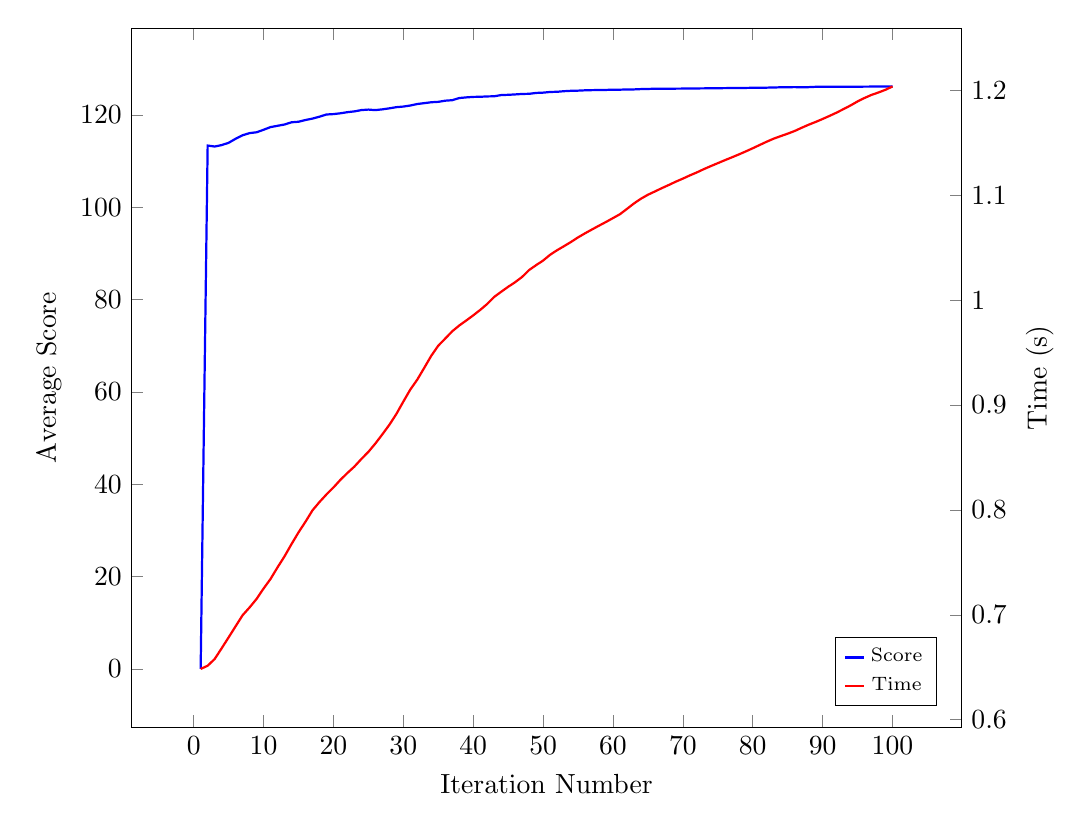
\begin{tikzpicture}
\begin{axis}[
    width=\textwidth,
    xlabel={Iteration Number},
    ylabel={Average Score},
    axis y line*=left,
]
\addplot[
    color=blue,
    style={thick}
    ]
    coordinates {
    (1, 0.0)(2, 113.34085713)(3, 113.13285712599999)(4, 113.44114284799998)(5, 113.93628571399998)(6, 114.81199999799999)(7, 115.57171428)(8, 116.03714285200002)(9, 116.21742857400004)(10, 116.75828571200002)(11, 117.34199999800002)(12, 117.62028572600003)(13, 117.90257142599998)(14, 118.38199999799997)(15, 118.49800000800002)(16, 118.87257143600002)(17, 119.17714285400002)(18, 119.595142854)(19, 120.06771428800003)(20, 120.15371428800005)(21, 120.32999999600001)(22, 120.57085713200001)(23, 120.74171428200002)(24, 121.02314285599999)(25, 121.13028571000001)(26, 121.01771428200004)(27, 121.18200000000006)(28, 121.40228571800006)(29, 121.65542857000004)(30, 121.78571428800005)(31, 122.01171428800005)(32, 122.33885715000004)(33, 122.52714286600006)(34, 122.72000000600008)(35, 122.80971429600008)(36, 123.05714286400008)(37, 123.16771428800007)(38, 123.62971428600007)(39, 123.77200000600007)(40, 123.87800000400006)(41, 123.90342857600005)(42, 123.98314286600005)(43, 124.01000000400006)(44, 124.27828572000006)(45, 124.32771429200007)(46, 124.41657144000008)(47, 124.51428572000006)(48, 124.54714286600007)(49, 124.73714286200006)(50, 124.80000001000005)(51, 124.94600001000006)(52, 124.98685715800009)(53, 125.11514287000007)(54, 125.19685715600005)(55, 125.23228572800006)(56, 125.30514287000005)(57, 125.34428572800006)(58, 125.36542858400007)(59, 125.39057143800002)(60, 125.43857144000006)(61, 125.44371429600005)(62, 125.48485715400007)(63, 125.50114286800006)(64, 125.56828572000002)(65, 125.60200000800003)(66, 125.64457143800003)(67, 125.64514286800004)(68, 125.64914286600003)(69, 125.66685715000004)(70, 125.67714286600004)(71, 125.67857143800003)(72, 125.71485714800004)(73, 125.72800000600003)(74, 125.74028572000005)(75, 125.76600000800005)(76, 125.77857143800003)(77, 125.79800000800003)(78, 125.82314286800003)(79, 125.82514287000004)(80, 125.85000000800004)(81, 125.85857143600005)(82, 125.88200001000003)(83, 125.91914287200004)(84, 125.95828572800004)(85, 125.97914286800004)(86, 125.99742858400003)(87, 125.96428572600004)(88, 125.99171429800005)(89, 126.06000001000005)(90, 126.05857143800004)(91, 126.07828572400004)(92, 126.06685715400006)(93, 126.06914286600005)(94, 126.08457143800005)(95, 126.09314286800006)(96, 126.10171429600005)(97, 126.11114286600004)(98, 126.12600001200006)(99, 126.13314286800005)(100, 126.13628572800008)    };
    \label{ls-graph-no-mins}
\end{axis}

\begin{axis}[
    width=\textwidth,
    ylabel near ticks, yticklabel pos=right,
    ylabel={Time (s)},
    legend pos = {south east},
    legend style={font=\scriptsize\selectfont,},
    legend image post style={scale=0.4},
    hide x axis,
    axis y line*=right,
]
\addlegendimage{/pgfplots/refstyle=ls-graph-no-mins, blue,style=thick}\addlegendentry{Score}
\addplot[
    color=red,
    style={thick}
    ]
    coordinates {
    (1, 0.6484239999999999)(2, 0.6514860000000001)(3, 0.6578380000000007)(4, 0.6680680000000001)(5, 0.6785079999999996)(6, 0.6890759999999995)(7, 0.6996239999999991)(8, 0.7070420000000003)(9, 0.715154)(10, 0.7250499999999999)(11, 0.7341979999999994)(12, 0.7452499999999993)(13, 0.7557399999999997)(14, 0.7674019999999997)(15, 0.7785680000000005)(16, 0.7887460000000001)(17, 0.7995779999999989)(18, 0.8075000000000003)(19, 0.8147479999999998)(20, 0.8213840000000001)(21, 0.8286939999999998)(22, 0.8352119999999998)(23, 0.8413279999999996)(24, 0.8485659999999997)(25, 0.8553300000000001)(26, 0.8632959999999997)(27, 0.8720539999999996)(28, 0.8811159999999999)(29, 0.891386)(30, 0.9032420000000009)(31, 0.9147340000000005)(32, 0.9242560000000001)(33, 0.9354919999999995)(34, 0.9469479999999997)(35, 0.9565439999999996)(36, 0.9633579999999996)(37, 0.9702779999999993)(38, 0.9757819999999988)(39, 0.9805380000000005)(40, 0.9854359999999998)(41, 0.990646)(42, 0.9962919999999997)(43, 1.0030420000000002)(44, 1.0079259999999992)(45, 1.0126820000000003)(46, 1.0170699999999995)(47, 1.0221019999999996)(48, 1.0286639999999991)(49, 1.033318)(50, 1.0376960000000004)(51, 1.0431919999999992)(52, 1.0475559999999993)(53, 1.0514260000000002)(54, 1.0554539999999997)(55, 1.059778)(56, 1.0636680000000003)(57, 1.0673420000000002)(58, 1.0709620000000004)(59, 1.0744840000000015)(60, 1.0781799999999988)(61, 1.0818700000000003)(62, 1.0869339999999992)(63, 1.0921120000000006)(64, 1.0966420000000012)(65, 1.1004280000000002)(66, 1.1035620000000004)(67, 1.1067599999999997)(68, 1.1097819999999996)(69, 1.112928000000001)(70, 1.1158099999999995)(71, 1.118867999999999)(72, 1.1217159999999993)(73, 1.124844000000001)(74, 1.1277419999999994)(75, 1.130534)(76, 1.1333380000000004)(77, 1.1360500000000007)(78, 1.1388140000000002)(79, 1.141731999999999)(80, 1.1447419999999997)(81, 1.1478940000000009)(82, 1.1510079999999994)(83, 1.1539019999999995)(84, 1.1563140000000003)(85, 1.1586559999999997)(86, 1.161204)(87, 1.164269999999999)(88, 1.1671879999999992)(89, 1.1698299999999988)(90, 1.1726500000000013)(91, 1.1756340000000016)(92, 1.17872)(93, 1.182118000000001)(94, 1.1855639999999994)(95, 1.189377999999999)(96, 1.1926920000000003)(97, 1.195632)(98, 1.1979300000000002)(99, 1.200514)(100, 1.203648)
    };
    \addlegendentry{Time}
\end{axis}
\end{tikzpicture}
\end{center}
\caption{LS}
\label{fig:graphs-unit-scoring-ls}
\end{subfigure}
\\[1ex]
\begin{subfigure}{.45\linewidth}
\begin{center}
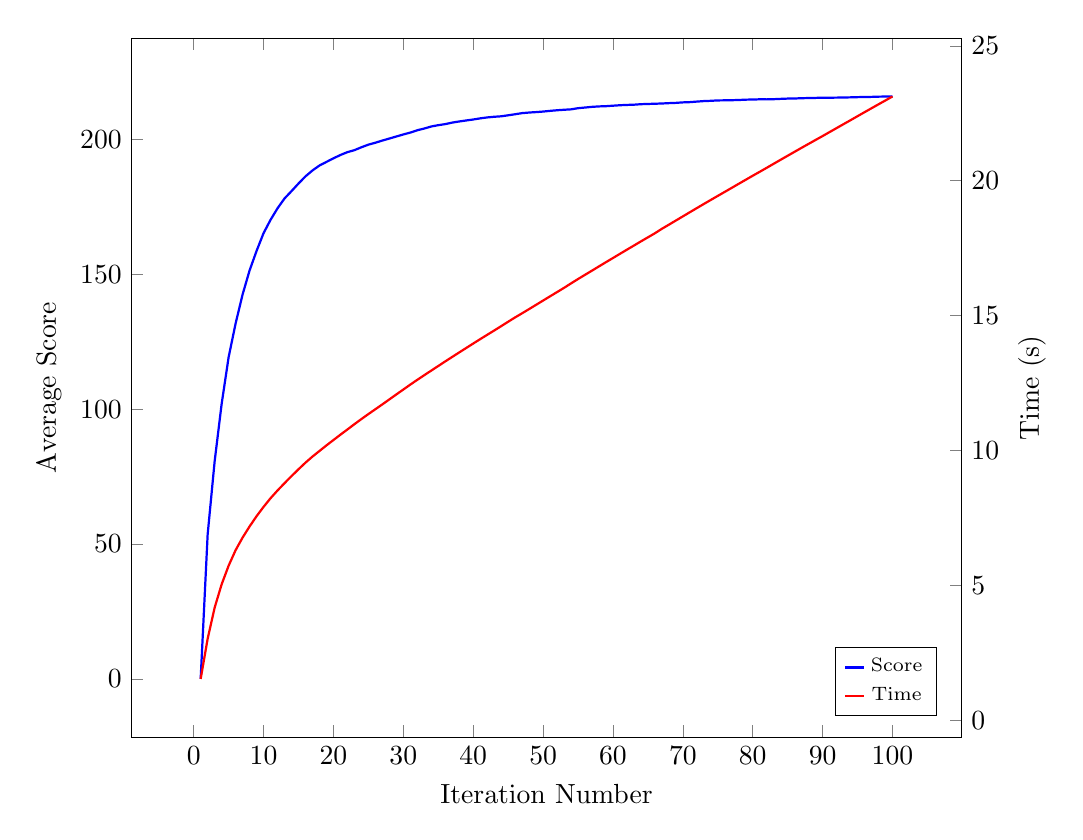
\begin{tikzpicture}
\begin{axis}[
    width=\textwidth,
    xlabel={Iteration Number},
    ylabel={Average Score},
    axis y line*=left,
]
\addplot[
    color=blue,
    style={thick}
    ]
    coordinates {
    (1, 0.0)(2, 53.54485713999996)(3, 80.64771426999998)(4, 101.89742856599999)(5, 119.24199999600005)(6, 131.7399999739999)(7, 142.49685714199998)(8, 151.40599999599996)(9, 158.63885713799996)(10, 165.21742856799995)(11, 170.16171427199995)(12, 174.43285714399994)(13, 178.07999998999992)(14, 180.800285716)(15, 183.61457141399993)(16, 186.26914284999992)(17, 188.46057141599994)(18, 190.29114284399992)(19, 191.62828570799994)(20, 192.95685712799994)(21, 194.193142852)(22, 195.24485713199996)(23, 195.97799998599993)(24, 197.05199998999993)(25, 198.02257142199994)(26, 198.73742857399992)(27, 199.54057142199986)(28, 200.28571427799992)(29, 201.04628571999996)(30, 201.802)(31, 202.500000006)(32, 203.36428572000003)(33, 204.00085713799996)(34, 204.760571426)(35, 205.24142858200003)(36, 205.6391428539999)(37, 206.19714284999995)(38, 206.61485715000003)(39, 206.988857142)(40, 207.34314286400004)(41, 207.77142857600006)(42, 208.11285714600007)(43, 208.35485713399993)(44, 208.52971428200001)(45, 208.90342856800004)(46, 209.292571424)(47, 209.70971428199994)(48, 209.92285714800002)(49, 210.08914287000005)(50, 210.28828572400005)(51, 210.54571429800006)(52, 210.77085714199998)(53, 210.95171428199998)(54, 211.105428574)(55, 211.53742856799997)(56, 211.78028569999992)(57, 212.03142856799997)(58, 212.196285712)(59, 212.28257142199996)(60, 212.45714285399998)(61, 212.634571428)(62, 212.74742856999998)(63, 212.833714288)(64, 213.01599999799998)(65, 213.10799999399995)(66, 213.18457142399996)(67, 213.27800000400003)(68, 213.409714288)(69, 213.506571434)(70, 213.68800000599998)(71, 213.78028570999996)(72, 213.98228570999996)(73, 214.16999999999996)(74, 214.268)(75, 214.41742856799996)(76, 214.44857142799998)(77, 214.49771428199995)(78, 214.57571428599996)(79, 214.69828571600002)(80, 214.75171428399997)(81, 214.82599999599998)(82, 214.80885713599992)(83, 214.87228570999997)(84, 214.9914285639999)(85, 215.09542856999997)(86, 215.13257142999998)(87, 215.23628570999998)(88, 215.29799999599996)(89, 215.35085713799995)(90, 215.43199999799995)(91, 215.43171428599996)(92, 215.45342856799996)(93, 215.508285714)(94, 215.552571428)(95, 215.63142857)(96, 215.68257142799996)(97, 215.72771428599998)(98, 215.81257142399997)(99, 215.85142857)(100, 215.87714286)    }; \label{ls-graph-budget-percent}
\end{axis}

\begin{axis}[
    width=\textwidth,
    ylabel near ticks, yticklabel pos=right,
    ylabel={Time (s)},
    legend pos = {south east},
    legend style={font=\scriptsize\selectfont,},
    legend image post style={scale=0.4},
    hide x axis,
    axis y line*=right,
]
\addlegendimage{/pgfplots/refstyle=ls-graph-budget-percent, blue,style=thick}\addlegendentry{Score}
\addplot[
    color=red,
    style={thick}
    ]
    coordinates {
(1, 1.5404639999999994)(2, 3.030628000000002)(3, 4.181223999999998)(4, 5.045037999999998)(5, 5.736461999999995)(6, 6.3113119999999965)(7, 6.778498000000003)(8, 7.190831999999996)(9, 7.569965999999998)(10, 7.915543999999994)(11, 8.236798000000002)(12, 8.523962000000001)(13, 8.794169999999998)(14, 9.055248)(15, 9.309724000000001)(16, 9.554674000000006)(17, 9.779929999999986)(18, 9.987127999999995)(19, 10.193661999999996)(20, 10.392640000000007)(21, 10.591159999999993)(22, 10.784546000000004)(23, 10.979709999999994)(24, 11.170064000000004)(25, 11.35469600000001)(26, 11.533738)(27, 11.714087999999997)(28, 11.897320000000015)(29, 12.082166000000004)(30, 12.263632000000001)(31, 12.447411999999998)(32, 12.622923999999996)(33, 12.796045999999993)(34, 12.965997999999995)(35, 13.135870000000008)(36, 13.306078000000007)(37, 13.472791999999991)(38, 13.638972000000006)(39, 13.803319999999998)(40, 13.968022000000007)(41, 14.130964)(42, 14.29088800000001)(43, 14.449906000000002)(44, 14.611660000000006)(45, 14.775492000000003)(46, 14.936703999999986)(47, 15.089251999999998)(48, 15.244979999999991)(49, 15.402916000000017)(50, 15.560572)(51, 15.718013999999997)(52, 15.874412000000001)(53, 16.03148999999999)(54, 16.196709999999992)(55, 16.358036000000002)(56, 16.514659999999985)(57, 16.669493999999993)(58, 16.827065999999988)(59, 16.983418000000004)(60, 17.13686600000002)(61, 17.292453999999996)(62, 17.44666399999999)(63, 17.599136)(64, 17.753107999999994)(65, 17.903282000000008)(66, 18.05397600000001)(67, 18.219918000000025)(68, 18.371512)(69, 18.52604999999999)(70, 18.679675999999997)(71, 18.833196000000015)(72, 18.986647999999978)(73, 19.138872000000006)(74, 19.289375999999983)(75, 19.438833999999996)(76, 19.587687999999982)(77, 19.73728600000002)(78, 19.88783400000001)(79, 20.036580000000015)(80, 20.185724000000018)(81, 20.331694000000006)(82, 20.47928)(83, 20.629487999999995)(84, 20.77885399999999)(85, 20.92689000000002)(86, 21.074596000000014)(87, 21.221957999999994)(88, 21.367570000000015)(89, 21.512194000000026)(90, 21.656795999999996)(91, 21.80439799999998)(92, 21.951017999999987)(93, 22.098104000000017)(94, 22.244324000000017)(95, 22.39271799999999)(96, 22.540094000000003)(97, 22.686846000000035)(98, 22.832402000000023)(99, 22.977423999999996)(100, 23.122468000000012)
    };
    \addlegendentry{Time}
\end{axis}
\end{tikzpicture}
\end{center}
\caption{LS + (Budget Allowance)}
\end{subfigure}
\hfill
\begin{subfigure}{.45\linewidth}
\begin{center}
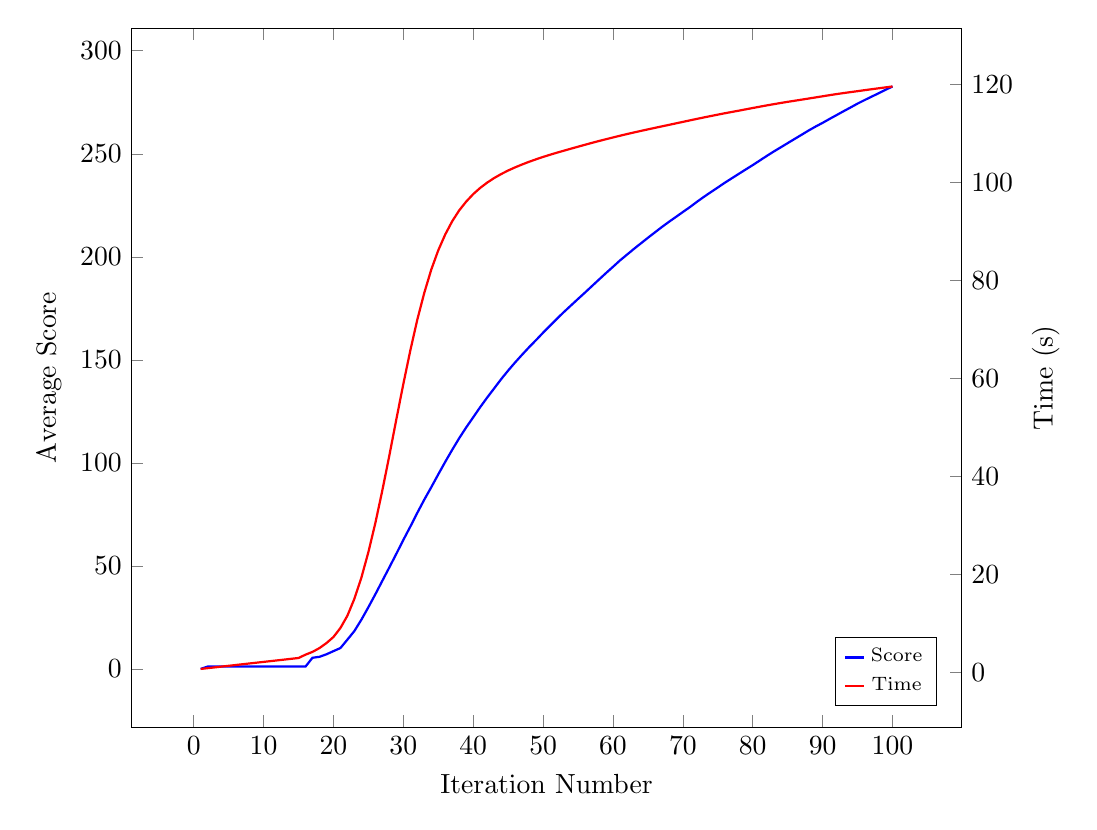
\begin{tikzpicture}
\begin{axis}[
    width=\textwidth,
    xlabel={Iteration Number},
    ylabel={Average Score},
    axis y line*=left,
]
\addplot[
    color=blue,
    style={thick}
    ]
    coordinates {
    (1, 0.0)(2, 1.1428570000000005)(3, 1.1428570000000005)(4, 1.1428570000000005)(5, 1.1428570000000005)(6, 1.1428570000000005)(7, 1.1428570000000005)(8, 1.1428570000000005)(9, 1.1428570000000005)(10, 1.1428570000000005)(11, 1.1428570000000005)(12, 1.1428570000000005)(13, 1.1428570000000005)(14, 1.1428570000000005)(15, 1.1428570000000005)(16, 1.1428570000000005)(17, 5.414857216000013)(18, 5.883428504000005)(19, 7.108571458000036)(20, 8.633714298000056)(21, 10.141142892000053)(22, 14.233714148000068)(23, 18.419428538000034)(24, 23.897142851999998)(25, 29.962285719999997)(26, 36.25942857399999)(27, 42.79657141400004)(28, 49.28685713600003)(29, 55.87428571799998)(30, 62.594857146000074)(31, 69.05657141000003)(32, 75.74514283599999)(33, 82.16628570399997)(34, 88.19942858400005)(35, 94.41657141599998)(36, 100.50971428599993)(37, 106.36685715200004)(38, 111.99485714600002)(39, 117.22285712199994)(40, 122.11714287400005)(41, 127.04571427599996)(42, 131.70571429400007)(43, 136.14285716400008)(44, 140.63485713199998)(45, 144.7988571219999)(46, 148.75199999800006)(47, 152.506285748)(48, 156.156571422)(49, 159.60799998799996)(50, 163.16971427399992)(51, 166.60685713199996)(52, 170.00628570399985)(53, 173.2828571360001)(54, 176.43142857199993)(55, 179.56685715000003)(56, 182.66057143800003)(57, 185.82228570800004)(58, 188.970285716)(59, 192.10228572400007)(60, 195.13942856799997)(61, 198.23371428800002)(62, 201.037142862)(63, 203.84628569999987)(64, 206.54171426999986)(65, 209.2325714139999)(66, 211.85657141999994)(67, 214.469714276)(68, 216.9542857280001)(69, 219.33028571600002)(70, 221.7485714540002)(71, 224.096000012)(72, 226.6600000100001)(73, 229.07485714199996)(74, 231.38742855799984)(75, 233.646285726)(76, 235.93485715600005)(77, 238.102285714)(78, 240.25085715600008)(79, 242.398857144)(80, 244.50571429199994)(81, 246.72057142399998)(82, 248.94114285800003)(83, 251.08000001000002)(84, 253.11885713799998)(85, 255.17085714799998)(86, 257.21314285399995)(87, 259.245714286)(88, 261.304571434)(89, 263.21885714199993)(90, 265.01542858000005)(91, 266.925142856)(92, 268.7880000200001)(93, 270.65600001800016)(94, 272.484000006)(95, 274.35314285399994)(96, 276.05942857199994)(97, 277.7245714420001)(98, 279.333714294)(99, 281.05542859800016)(100, 282.66971429800003)    }; \label{ls-graph-incremental}
\end{axis}

\begin{axis}[
    width=\textwidth,
    ylabel near ticks, yticklabel pos=right,
    ylabel={Time (s)},
    legend pos = {south east},
    legend style={font=\scriptsize\selectfont},
    legend image post style={scale=0.4},
    hide x axis,
    axis y line*=right,
]
\addlegendimage{/pgfplots/refstyle=ls-graph-incremental, blue,style=thick}\addlegendentry{Score}
\addplot[
    color=red,
    style={thick}
    ]
    coordinates {
(1, 0.6553780000000007)(2, 0.8145339999999994)(3, 0.9736880000000008)(4, 1.133602000000002)(5, 1.2937079999999974)(6, 1.454020000000001)(7, 1.6141880000000022)(8, 1.7739779999999983)(9, 1.9332999999999967)(10, 2.0923160000000007)(11, 2.2512020000000015)(12, 2.4099279999999994)(13, 2.569098000000002)(14, 2.7278939999999987)(15, 2.8868360000000006)(16, 3.565115999999996)(17, 4.133447999999998)(18, 4.9078959999999965)(19, 5.931039999999992)(20, 7.170333999999998)(21, 9.014160000000002)(22, 11.527971999999993)(23, 14.976956000000005)(24, 19.294753999999976)(25, 24.49373600000001)(26, 30.447487999999986)(27, 37.11408799999997)(28, 44.22119600000003)(29, 51.59153)(30, 58.79706399999997)(31, 65.64260600000003)(32, 71.93420800000005)(33, 77.40983799999997)(34, 82.15846599999993)(35, 86.08474399999994)(36, 89.32948999999992)(37, 92.03269800000001)(38, 94.244002)(39, 96.03647800000007)(40, 97.55355000000013)(41, 98.82415200000004)(42, 99.90436400000003)(43, 100.83597400000004)(44, 101.64726799999995)(45, 102.37428600000004)(46, 103.01933199999989)(47, 103.60660799999991)(48, 104.15785799999988)(49, 104.66250599999998)(50, 105.14375800000002)(51, 105.593072)(52, 106.01980600000016)(53, 106.42931400000003)(54, 106.83500600000005)(55, 107.23226799999995)(56, 107.62728399999997)(57, 108.01994)(58, 108.39690200000013)(59, 108.75836800000006)(60, 109.11838199999985)(61, 109.46851800000012)(62, 109.81155199999996)(63, 110.13977800000008)(64, 110.45737799999996)(65, 110.76974799999998)(66, 111.07706600000006)(67, 111.38328600000004)(68, 111.68629599999991)(69, 111.99076400000007)(70, 112.29828000000003)(71, 112.60102600000003)(72, 112.9068540000001)(73, 113.20118799999997)(74, 113.49045799999999)(75, 113.77756000000008)(76, 114.05764600000002)(77, 114.32137399999995)(78, 114.58435000000006)(79, 114.85938999999998)(80, 115.1284100000001)(81, 115.39673399999998)(82, 115.65732200000006)(83, 115.90934999999989)(84, 116.15202600000002)(85, 116.38925200000013)(86, 116.61209599999992)(87, 116.83666599999987)(88, 117.06390800000005)(89, 117.29110199999995)(90, 117.52334999999998)(91, 117.75103200000001)(92, 117.97224800000004)(93, 118.17810599999993)(94, 118.37594199999995)(95, 118.56767599999992)(96, 118.76787799999998)(97, 118.96026999999984)(98, 119.14996399999991)(99, 119.3383299999999)(100, 119.52416600000016)    };
\addlegendentry{Time}
\end{axis}
\end{tikzpicture}
\end{center}
\caption{LS + (Incremental Budget) \label{fig:graph-inc}}
\end{subfigure}
\\[1ex]
\begin{subfigure}{.45\linewidth}
\begin{center}
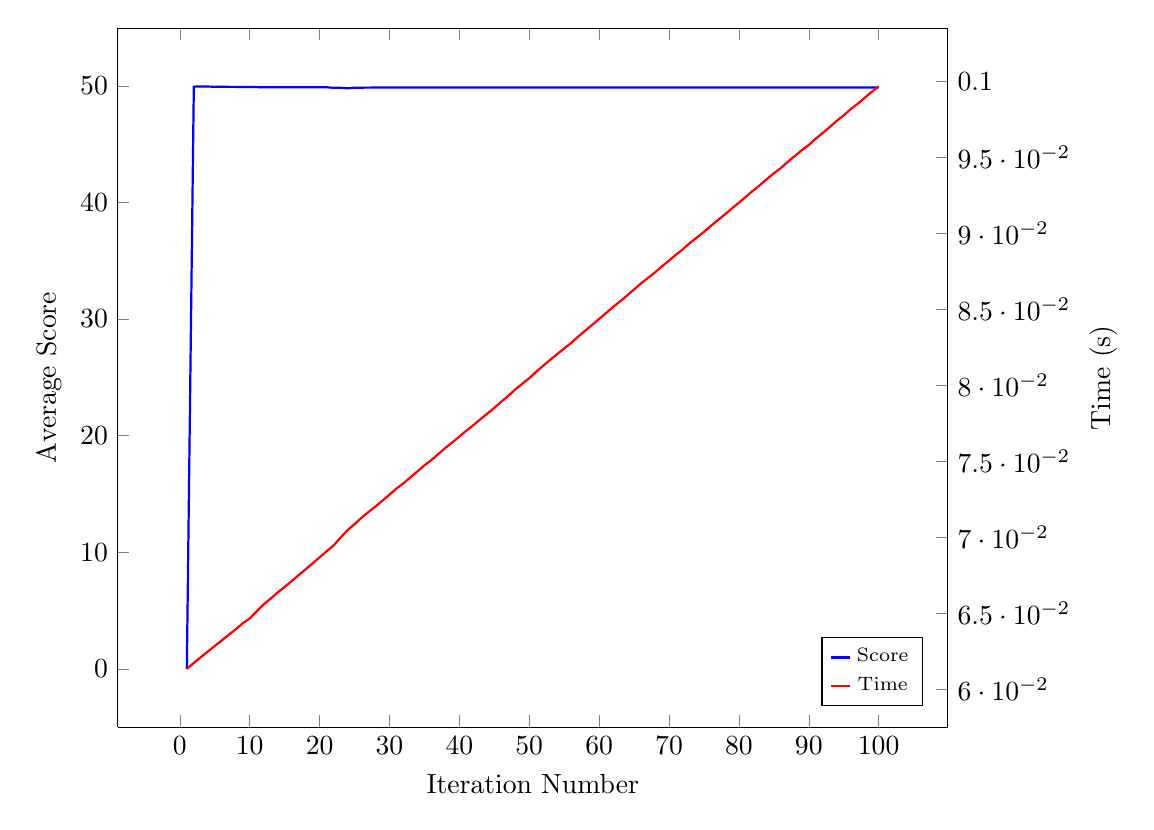
\begin{tikzpicture}
\begin{axis}[
    width=\textwidth,
    xlabel={Iteration Number},
    ylabel={Average Score},
    axis y line*=left,
]
\addplot[
    color=blue,
    style={thick}
    ]
    coordinates {
    (1, 0.0)(2, 49.93028571600001)(3, 49.94514285600001)(4, 49.93600000200001)(5, 49.92400000200001)(6, 49.91771428800001)(7, 49.912000002000006)(8, 49.912000002000006)(9, 49.89714286000001)(10, 49.892571432000004)(11, 49.89200000200001)(12, 49.869714288000004)(13, 49.87857143)(14, 49.87857143)(15, 49.87857143)(16, 49.87857143)(17, 49.87857143)(18, 49.87857143)(19, 49.87857143)(20, 49.87857143)(21, 49.87857143)(22, 49.83171428600001)(23, 49.83457143000001)(24, 49.78800000200002)(25, 49.843714286000015)(26, 49.843714286000015)(27, 49.84685714400002)(28, 49.850285716000016)(29, 49.850285716000016)(30, 49.850285716000016)(31, 49.850285716000016)(32, 49.850285716000016)(33, 49.850285716000016)(34, 49.850285716000016)(35, 49.850285716000016)(36, 49.85314285800001)(37, 49.85314285800001)(38, 49.85314285800001)(39, 49.85314285800001)(40, 49.85314285800001)(41, 49.85314285800001)(42, 49.85314285800001)(43, 49.85314285800001)(44, 49.85314285800001)(45, 49.85314285800001)(46, 49.85314285800001)(47, 49.85314285800001)(48, 49.85314285800001)(49, 49.85314285800001)(50, 49.85314285800001)(51, 49.85314285800001)(52, 49.85314285800001)(53, 49.85314285800001)(54, 49.85314285800001)(55, 49.85314285800001)(56, 49.85314285800001)(57, 49.85314285800001)(58, 49.85314285800001)(59, 49.85314285800001)(60, 49.85314285800001)(61, 49.85314285800001)(62, 49.85314285800001)(63, 49.85314285800001)(64, 49.85314285800001)(65, 49.85314285800001)(66, 49.85314285800001)(67, 49.85314285800001)(68, 49.85314285800001)(69, 49.85314285800001)(70, 49.85314285800001)(71, 49.85314285800001)(72, 49.85314285800001)(73, 49.85314285800001)(74, 49.85314285800001)(75, 49.85314285800001)(76, 49.85314285800001)(77, 49.85314285800001)(78, 49.85314285800001)(79, 49.85314285800001)(80, 49.85314285800001)(81, 49.85314285800001)(82, 49.85314285800001)(83, 49.85314285800001)(84, 49.85314285800001)(85, 49.85314285800001)(86, 49.85314285800001)(87, 49.85314285800001)(88, 49.85314285800001)(89, 49.85314285800001)(90, 49.85314285800001)(91, 49.85314285800001)(92, 49.85314285800001)(93, 49.85314285800001)(94, 49.85314285800001)(95, 49.85314285800001)(96, 49.85314285800001)(97, 49.85314285800001)(98, 49.85314285800001)(99, 49.85314285800001)(100, 49.85314285800001)    }; \label{ls-graph-normal}
\end{axis}

\begin{axis}[
    width=\textwidth,
    ylabel near ticks, yticklabel pos=right,
    ylabel={Time (s)},
    legend pos = {south east},
    legend style={font=\scriptsize\selectfont,},
    legend image post style={scale=0.4},
    hide x axis,
    axis y line*=right,
]
\addlegendimage{/pgfplots/refstyle=ls-graph-budget-percent, blue,style=thick}\addlegendentry{Score}
\addplot[
    color=red,
    style={thick}
    ]
    coordinates {
(1, 0.06131999999999988)(2, 0.061715999999999785)(3, 0.06209799999999986)(4, 0.06246599999999992)(5, 0.062836)(6, 0.06320000000000005)(7, 0.0635720000000001)(8, 0.06393000000000006)(9, 0.06433000000000004)(10, 0.06464600000000001)(11, 0.06511599999999995)(12, 0.06557400000000002)(13, 0.06595200000000004)(14, 0.06635200000000008)(15, 0.0667160000000001)(16, 0.06710400000000008)(17, 0.06749200000000007)(18, 0.06787600000000006)(19, 0.06827400000000008)(20, 0.0686620000000001)(21, 0.06906200000000014)(22, 0.06944600000000016)(23, 0.06996400000000015)(24, 0.07045000000000008)(25, 0.07085200000000011)(26, 0.07127200000000013)(27, 0.07164800000000023)(28, 0.07201600000000023)(29, 0.07240000000000016)(30, 0.07278600000000014)(31, 0.07319400000000009)(32, 0.07353600000000013)(33, 0.07393200000000018)(34, 0.07431600000000017)(35, 0.0747200000000002)(36, 0.07507000000000025)(37, 0.0754680000000002)(38, 0.07586200000000018)(39, 0.0762320000000001)(40, 0.07661400000000015)(41, 0.07700400000000017)(42, 0.07736200000000024)(43, 0.07775000000000025)(44, 0.07812400000000023)(45, 0.07850200000000024)(46, 0.0789020000000002)(47, 0.07929000000000017)(48, 0.07971800000000012)(49, 0.0800880000000001)(50, 0.08045600000000012)(51, 0.08088600000000024)(52, 0.08126800000000024)(53, 0.08166600000000022)(54, 0.0820400000000002)(55, 0.08241200000000015)(56, 0.08277800000000017)(57, 0.08319200000000013)(58, 0.08358000000000014)(59, 0.08396200000000016)(60, 0.08435200000000012)(61, 0.08474600000000014)(62, 0.08514200000000008)(63, 0.08551200000000012)(64, 0.0858940000000001)(65, 0.08630000000000013)(66, 0.08669000000000017)(67, 0.08705600000000013)(68, 0.08742000000000014)(69, 0.08781400000000007)(70, 0.08819600000000011)(71, 0.08858400000000015)(72, 0.08894600000000018)(73, 0.08935600000000024)(74, 0.08971400000000021)(75, 0.09008600000000012)(76, 0.09048000000000009)(77, 0.09086000000000008)(78, 0.09123200000000006)(79, 0.09162600000000007)(80, 0.09200000000000015)(81, 0.09239200000000032)(82, 0.09279000000000025)(83, 0.09315200000000014)(84, 0.09356200000000005)(85, 0.09393400000000006)(86, 0.09428400000000008)(87, 0.09469600000000016)(88, 0.09507600000000016)(89, 0.09545600000000022)(90, 0.0958000000000002)(91, 0.09622000000000012)(92, 0.0965960000000001)(93, 0.09697600000000009)(94, 0.09739200000000009)(95, 0.09774800000000004)(96, 0.09816200000000007)(97, 0.09850800000000011)(98, 0.09890400000000006)(99, 0.09930000000000004)(100, 0.09965000000000003)
    };
    \addlegendentry{Time}
\end{axis}
\end{tikzpicture}
\end{center}
\caption{LS + (Arc Restrictions)}
\end{subfigure}
\hfill
\begin{subfigure}{.45\linewidth}
\begin{center}
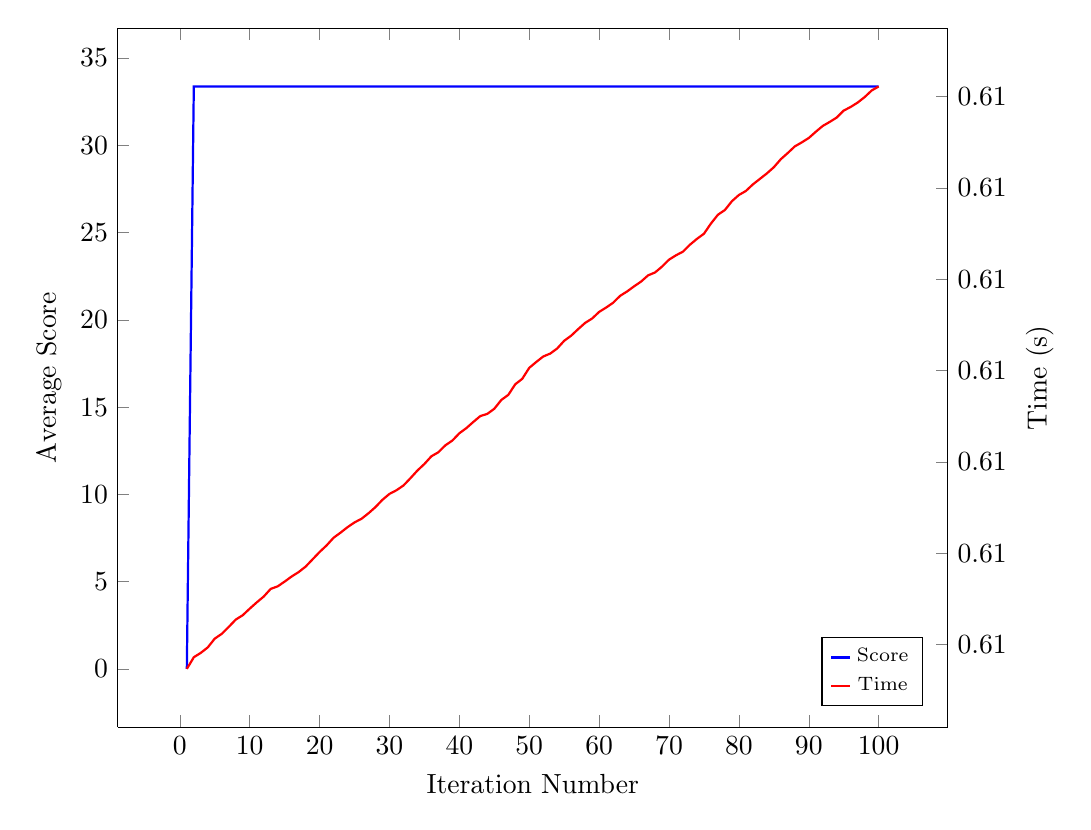
\begin{tikzpicture}
\begin{axis}[
    width=\textwidth,
    xlabel={Iteration Number},
    ylabel={Average Score},
    axis y line*=left,
]
\addplot[
    color=blue,
    style={thick}
    ]
    coordinates {
    (1, 0.0)(2, 33.36999997199997)(3, 33.36999997199997)(4, 33.36999997199997)(5, 33.36999997199997)(6, 33.36999997199997)(7, 33.36999997199997)(8, 33.36999997199997)(9, 33.36999997199997)(10, 33.36999997199997)(11, 33.36999997199997)(12, 33.36999997199997)(13, 33.36999997199997)(14, 33.36999997199997)(15, 33.36999997199997)(16, 33.36999997199997)(17, 33.36999997199997)(18, 33.36999997199997)(19, 33.36999997199997)(20, 33.36999997199997)(21, 33.36999997199997)(22, 33.36999997199997)(23, 33.36999997199997)(24, 33.36999997199997)(25, 33.36999997199997)(26, 33.36999997199997)(27, 33.36999997199997)(28, 33.36999997199997)(29, 33.36999997199997)(30, 33.36999997199997)(31, 33.36999997199997)(32, 33.36999997199997)(33, 33.36999997199997)(34, 33.36999997199997)(35, 33.36999997199997)(36, 33.36999997199997)(37, 33.36999997199997)(38, 33.36999997199997)(39, 33.36999997199997)(40, 33.36999997199997)(41, 33.36999997199997)(42, 33.36999997199997)(43, 33.36999997199997)(44, 33.36999997199997)(45, 33.36999997199997)(46, 33.36999997199997)(47, 33.36999997199997)(48, 33.36999997199997)(49, 33.36999997199997)(50, 33.36999997199997)(51, 33.36999997199997)(52, 33.36999997199997)(53, 33.36999997199997)(54, 33.36999997199997)(55, 33.36999997199997)(56, 33.36999997199997)(57, 33.36999997199997)(58, 33.36999997199997)(59, 33.36999997199997)(60, 33.36999997199997)(61, 33.36999997199997)(62, 33.36999997199997)(63, 33.36999997199997)(64, 33.36999997199997)(65, 33.36999997199997)(66, 33.36999997199997)(67, 33.36999997199997)(68, 33.36999997199997)(69, 33.36999997199997)(70, 33.36999997199997)(71, 33.36999997199997)(72, 33.36999997199997)(73, 33.36999997199997)(74, 33.36999997199997)(75, 33.36999997199997)(76, 33.36999997199997)(77, 33.36999997199997)(78, 33.36999997199997)(79, 33.36999997199997)(80, 33.36999997199997)(81, 33.36999997199997)(82, 33.36999997199997)(83, 33.36999997199997)(84, 33.36999997199997)(85, 33.36999997199997)(86, 33.36999997199997)(87, 33.36999997199997)(88, 33.36999997199997)(89, 33.36999997199997)(90, 33.36999997199997)(91, 33.36999997199997)(92, 33.36999997199997)(93, 33.36999997199997)(94, 33.36999997199997)(95, 33.36999997199997)(96, 33.36999997199997)(97, 33.36999997199997)(98, 33.36999997199997)(99, 33.36999997199997)(100, 33.36999997199997)    }; \label{ls-graph-incremental}
\end{axis}

\begin{axis}[
    width=\textwidth,
    ylabel near ticks, yticklabel pos=right,
    ylabel={Time (s)},
    legend pos = {south east},
    legend style={font=\scriptsize\selectfont},
    legend image post style={scale=0.4},
    hide x axis,
    axis y line*=right,
]
\addlegendimage{/pgfplots/refstyle=ls-graph-incremental, blue,style=thick}\addlegendentry{Score}
\addplot[
    color=red,
    style={thick}
    ]
    coordinates {
(1, 0.6053679999999996)(2, 0.6054319999999993)(3, 0.6054559999999993)(4, 0.6054859999999994)(5, 0.6055339999999995)(6, 0.6055599999999994)(7, 0.6055979999999992)(8, 0.6056379999999996)(9, 0.6056619999999996)(10, 0.6056979999999996)(11, 0.6057319999999995)(12, 0.6057639999999994)(13, 0.6058059999999993)(14, 0.6058199999999992)(15, 0.6058459999999994)(16, 0.6058739999999995)(17, 0.6058979999999996)(18, 0.6059279999999997)(19, 0.6059679999999996)(20, 0.6060079999999997)(21, 0.6060439999999998)(22, 0.6060859999999997)(23, 0.6061139999999997)(24, 0.6061439999999998)(25, 0.60617)(26, 0.6061899999999998)(27, 0.6062199999999999)(28, 0.6062539999999997)(29, 0.6062940000000001)(30, 0.6063259999999999)(31, 0.606346)(32, 0.6063719999999999)(33, 0.6064119999999997)(34, 0.6064539999999996)(35, 0.6064899999999996)(36, 0.6065319999999997)(37, 0.6065539999999996)(38, 0.6065919999999997)(39, 0.6066179999999995)(40, 0.6066579999999997)(41, 0.6066859999999998)(42, 0.60672)(43, 0.606752)(44, 0.606764)(45, 0.6067919999999999)(46, 0.6068400000000002)(47, 0.6068680000000001)(48, 0.6069260000000002)(49, 0.606956)(50, 0.6070160000000003)(51, 0.6070480000000001)(52, 0.6070780000000001)(53, 0.6070940000000001)(54, 0.6071220000000002)(55, 0.6071640000000001)(56, 0.6071919999999998)(57, 0.6072279999999998)(58, 0.6072619999999999)(59, 0.607286)(60, 0.607322)(61, 0.6073460000000002)(62, 0.607372)(63, 0.6074099999999998)(64, 0.6074339999999997)(65, 0.6074619999999997)(66, 0.6074879999999998)(67, 0.6075219999999998)(68, 0.6075379999999998)(69, 0.6075699999999997)(70, 0.6076079999999996)(71, 0.6076319999999997)(72, 0.6076519999999997)(73, 0.6076899999999997)(74, 0.6077219999999998)(75, 0.6077499999999997)(76, 0.6078059999999997)(77, 0.6078539999999996)(78, 0.6078799999999998)(79, 0.6079279999999999)(80, 0.6079619999999998)(81, 0.6079839999999999)(82, 0.6080199999999999)(83, 0.6080499999999999)(84, 0.6080799999999997)(85, 0.6081139999999999)(86, 0.6081579999999996)(87, 0.6081919999999996)(88, 0.6082279999999995)(89, 0.6082499999999995)(90, 0.6082739999999995)(91, 0.6083079999999996)(92, 0.6083399999999998)(93, 0.608362)(94, 0.6083859999999999)(95, 0.608424)(96, 0.6084439999999999)(97, 0.6084679999999998)(98, 0.6084979999999998)(99, 0.6085339999999999)(100, 0.6085559999999999)    };
\addlegendentry{Time}
\end{axis}
\end{tikzpicture}
\end{center}
\caption{LS + (No Backtracking)}
\end{subfigure}
\caption{Algorithm performance with unit scoring.}
\label{fig:graphs-unit-scoring}
\end{figure}


% COMBINED GRAPH
\begin{figure}
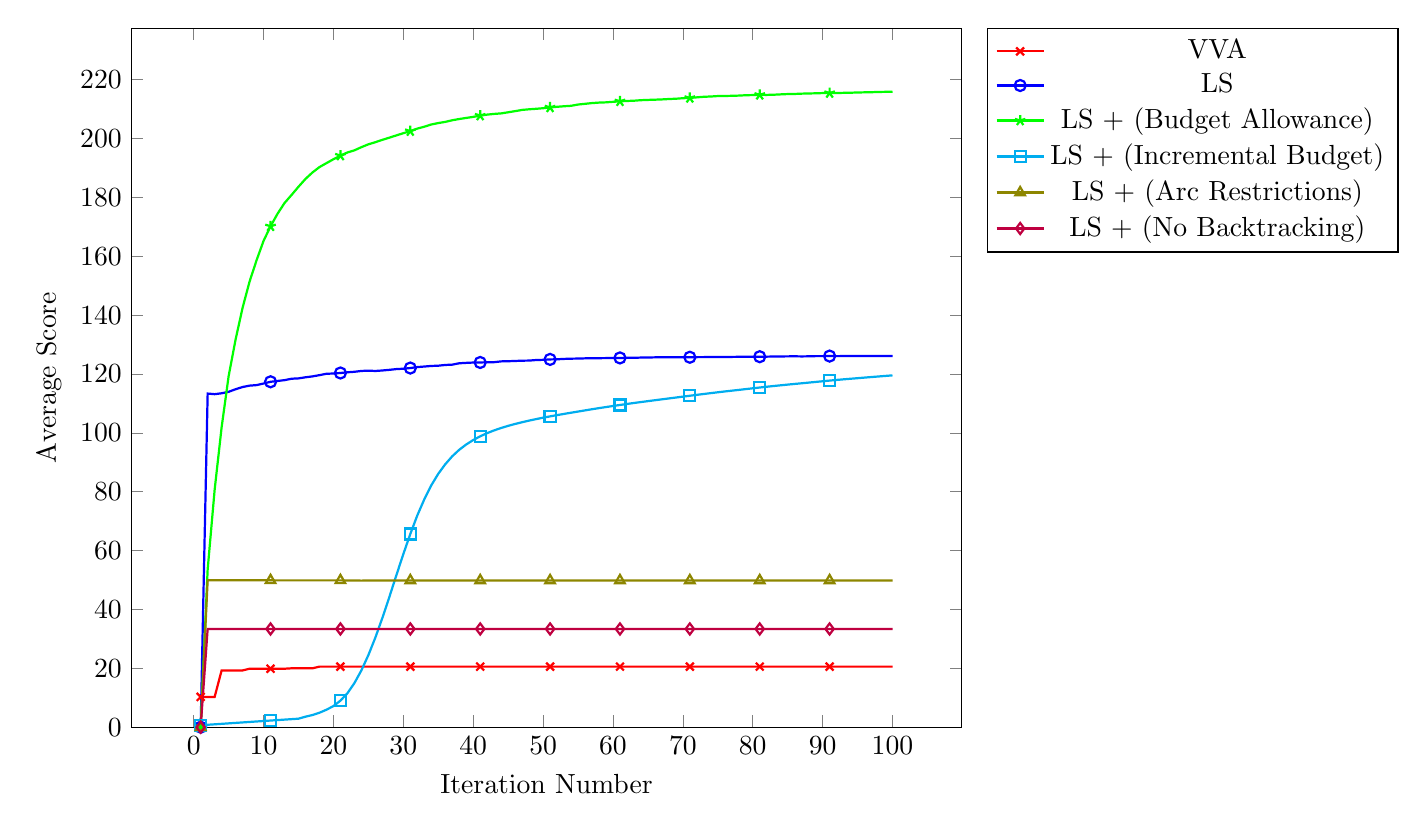
\begin{tikzpicture}
\begin{axis}[
    width=\textwidth,
    xlabel={Iteration Number},
    ylabel={Average Score},
    ymin=0,
    legend pos = {outer north east},
    mark repeat={10}
]

\addplot[
    color=red,
    style={thick},
    mark=x
    ]
    coordinates {
    (1, 10.285714000000002)(2, 10.285714000000002)(3, 10.285714000000002)(4, 19.285713999999995)(5, 19.285713999999995)(6, 19.285713999999995)(7, 19.285713999999995)(8, 19.857142999999997)(9, 19.857142999999997)(10, 19.857142999999997)(11, 19.857142999999997)(12, 19.857142999999997)(13, 19.857142999999997)(14, 20.0)(15, 20.0)(16, 20.0)(17, 20.0)(18, 20.571429000000002)(19, 20.571429000000002)(20, 20.571429000000002)(21, 20.571429000000002)(22, 20.571429000000002)(23, 20.571429000000002)(24, 20.571429000000002)(25, 20.571429000000002)(26, 20.571429000000002)(27, 20.571429000000002)(28, 20.571429000000002)(29, 20.571429000000002)(30, 20.571429000000002)(31, 20.571429000000002)(32, 20.571429000000002)(33, 20.571429000000002)(34, 20.571429000000002)(35, 20.571429000000002)(36, 20.571429000000002)(37, 20.571429000000002)(38, 20.571429000000002)(39, 20.571429000000002)(40, 20.571429000000002)(41, 20.571429000000002)(42, 20.571429000000002)(43, 20.571429000000002)(44, 20.571429000000002)(45, 20.571429000000002)(46, 20.571429000000002)(47, 20.571429000000002)(48, 20.571429000000002)(49, 20.571429000000002)(50, 20.571429000000002)(51, 20.571429000000002)(52, 20.571429000000002)(53, 20.571429000000002)(54, 20.571429000000002)(55, 20.571429000000002)(56, 20.571429000000002)(57, 20.571429000000002)(58, 20.571429000000002)(59, 20.571429000000002)(60, 20.571429000000002)(61, 20.571429000000002)(62, 20.571429000000002)(63, 20.571429000000002)(64, 20.571429000000002)(65, 20.571429000000002)(66, 20.571429000000002)(67, 20.571429000000002)(68, 20.571429000000002)(69, 20.571429000000002)(70, 20.571429000000002)(71, 20.571429000000002)(72, 20.571429000000002)(73, 20.571429000000002)(74, 20.571429000000002)(75, 20.571429000000002)(76, 20.571429000000002)(77, 20.571429000000002)(78, 20.571429000000002)(79, 20.571429000000002)(80, 20.571429000000002)(81, 20.571429000000002)(82, 20.571429000000002)(83, 20.571429000000002)(84, 20.571429000000002)(85, 20.571429000000002)(86, 20.571429000000002)(87, 20.571429000000002)(88, 20.571429000000002)(89, 20.571429000000002)(90, 20.571429000000002)(91, 20.571429000000002)(92, 20.571429000000002)(93, 20.571429000000002)(94, 20.571429000000002)(95, 20.571429000000002)(96, 20.571429000000002)(97, 20.571429000000002)(98, 20.571429000000002)(99, 20.571429000000002)(100, 20.571429000000002)
    };
    
\addlegendentry{VVA}

\addplot[
    color=blue,
    style={thick},
    mark=o
    ]
    coordinates {
    (1, 0.0)(2, 113.34085713)(3, 113.13285712599999)(4, 113.44114284799998)(5, 113.93628571399998)(6, 114.81199999799999)(7, 115.57171428)(8, 116.03714285200002)(9, 116.21742857400004)(10, 116.75828571200002)(11, 117.34199999800002)(12, 117.62028572600003)(13, 117.90257142599998)(14, 118.38199999799997)(15, 118.49800000800002)(16, 118.87257143600002)(17, 119.17714285400002)(18, 119.595142854)(19, 120.06771428800003)(20, 120.15371428800005)(21, 120.32999999600001)(22, 120.57085713200001)(23, 120.74171428200002)(24, 121.02314285599999)(25, 121.13028571000001)(26, 121.01771428200004)(27, 121.18200000000006)(28, 121.40228571800006)(29, 121.65542857000004)(30, 121.78571428800005)(31, 122.01171428800005)(32, 122.33885715000004)(33, 122.52714286600006)(34, 122.72000000600008)(35, 122.80971429600008)(36, 123.05714286400008)(37, 123.16771428800007)(38, 123.62971428600007)(39, 123.77200000600007)(40, 123.87800000400006)(41, 123.90342857600005)(42, 123.98314286600005)(43, 124.01000000400006)(44, 124.27828572000006)(45, 124.32771429200007)(46, 124.41657144000008)(47, 124.51428572000006)(48, 124.54714286600007)(49, 124.73714286200006)(50, 124.80000001000005)(51, 124.94600001000006)(52, 124.98685715800009)(53, 125.11514287000007)(54, 125.19685715600005)(55, 125.23228572800006)(56, 125.30514287000005)(57, 125.34428572800006)(58, 125.36542858400007)(59, 125.39057143800002)(60, 125.43857144000006)(61, 125.44371429600005)(62, 125.48485715400007)(63, 125.50114286800006)(64, 125.56828572000002)(65, 125.60200000800003)(66, 125.64457143800003)(67, 125.64514286800004)(68, 125.64914286600003)(69, 125.66685715000004)(70, 125.67714286600004)(71, 125.67857143800003)(72, 125.71485714800004)(73, 125.72800000600003)(74, 125.74028572000005)(75, 125.76600000800005)(76, 125.77857143800003)(77, 125.79800000800003)(78, 125.82314286800003)(79, 125.82514287000004)(80, 125.85000000800004)(81, 125.85857143600005)(82, 125.88200001000003)(83, 125.91914287200004)(84, 125.95828572800004)(85, 125.97914286800004)(86, 125.99742858400003)(87, 125.96428572600004)(88, 125.99171429800005)(89, 126.06000001000005)(90, 126.05857143800004)(91, 126.07828572400004)(92, 126.06685715400006)(93, 126.06914286600005)(94, 126.08457143800005)(95, 126.09314286800006)(96, 126.10171429600005)(97, 126.11114286600004)(98, 126.12600001200006)(99, 126.13314286800005)(100, 126.13628572800008)    };
\addlegendentry{LS}

\addplot[
    color=green,
    style={thick},
    mark=star
    ]
    coordinates {
    (1, 0.0)(2, 53.54485713999996)(3, 80.64771426999998)(4, 101.89742856599999)(5, 119.24199999600005)(6, 131.7399999739999)(7, 142.49685714199998)(8, 151.40599999599996)(9, 158.63885713799996)(10, 165.21742856799995)(11, 170.16171427199995)(12, 174.43285714399994)(13, 178.07999998999992)(14, 180.800285716)(15, 183.61457141399993)(16, 186.26914284999992)(17, 188.46057141599994)(18, 190.29114284399992)(19, 191.62828570799994)(20, 192.95685712799994)(21, 194.193142852)(22, 195.24485713199996)(23, 195.97799998599993)(24, 197.05199998999993)(25, 198.02257142199994)(26, 198.73742857399992)(27, 199.54057142199986)(28, 200.28571427799992)(29, 201.04628571999996)(30, 201.802)(31, 202.500000006)(32, 203.36428572000003)(33, 204.00085713799996)(34, 204.760571426)(35, 205.24142858200003)(36, 205.6391428539999)(37, 206.19714284999995)(38, 206.61485715000003)(39, 206.988857142)(40, 207.34314286400004)(41, 207.77142857600006)(42, 208.11285714600007)(43, 208.35485713399993)(44, 208.52971428200001)(45, 208.90342856800004)(46, 209.292571424)(47, 209.70971428199994)(48, 209.92285714800002)(49, 210.08914287000005)(50, 210.28828572400005)(51, 210.54571429800006)(52, 210.77085714199998)(53, 210.95171428199998)(54, 211.105428574)(55, 211.53742856799997)(56, 211.78028569999992)(57, 212.03142856799997)(58, 212.196285712)(59, 212.28257142199996)(60, 212.45714285399998)(61, 212.634571428)(62, 212.74742856999998)(63, 212.833714288)(64, 213.01599999799998)(65, 213.10799999399995)(66, 213.18457142399996)(67, 213.27800000400003)(68, 213.409714288)(69, 213.506571434)(70, 213.68800000599998)(71, 213.78028570999996)(72, 213.98228570999996)(73, 214.16999999999996)(74, 214.268)(75, 214.41742856799996)(76, 214.44857142799998)(77, 214.49771428199995)(78, 214.57571428599996)(79, 214.69828571600002)(80, 214.75171428399997)(81, 214.82599999599998)(82, 214.80885713599992)(83, 214.87228570999997)(84, 214.9914285639999)(85, 215.09542856999997)(86, 215.13257142999998)(87, 215.23628570999998)(88, 215.29799999599996)(89, 215.35085713799995)(90, 215.43199999799995)(91, 215.43171428599996)(92, 215.45342856799996)(93, 215.508285714)(94, 215.552571428)(95, 215.63142857)(96, 215.68257142799996)(97, 215.72771428599998)(98, 215.81257142399997)(99, 215.85142857)(100, 215.87714286)    };
\addlegendentry{LS + (Budget Allowance)}

\addplot[
    color=cyan,
    style={thick},
    mark=square
    ]
    coordinates {
(1, 0.6553780000000007)(2, 0.8145339999999994)(3, 0.9736880000000008)(4, 1.133602000000002)(5, 1.2937079999999974)(6, 1.454020000000001)(7, 1.6141880000000022)(8, 1.7739779999999983)(9, 1.9332999999999967)(10, 2.0923160000000007)(11, 2.2512020000000015)(12, 2.4099279999999994)(13, 2.569098000000002)(14, 2.7278939999999987)(15, 2.8868360000000006)(16, 3.565115999999996)(17, 4.133447999999998)(18, 4.9078959999999965)(19, 5.931039999999992)(20, 7.170333999999998)(21, 9.014160000000002)(22, 11.527971999999993)(23, 14.976956000000005)(24, 19.294753999999976)(25, 24.49373600000001)(26, 30.447487999999986)(27, 37.11408799999997)(28, 44.22119600000003)(29, 51.59153)(30, 58.79706399999997)(31, 65.64260600000003)(32, 71.93420800000005)(33, 77.40983799999997)(34, 82.15846599999993)(35, 86.08474399999994)(36, 89.32948999999992)(37, 92.03269800000001)(38, 94.244002)(39, 96.03647800000007)(40, 97.55355000000013)(41, 98.82415200000004)(42, 99.90436400000003)(43, 100.83597400000004)(44, 101.64726799999995)(45, 102.37428600000004)(46, 103.01933199999989)(47, 103.60660799999991)(48, 104.15785799999988)(49, 104.66250599999998)(50, 105.14375800000002)(51, 105.593072)(52, 106.01980600000016)(53, 106.42931400000003)(54, 106.83500600000005)(55, 107.23226799999995)(56, 107.62728399999997)(57, 108.01994)(58, 108.39690200000013)(59, 108.75836800000006)(60, 109.11838199999985)(61, 109.46851800000012)(62, 109.81155199999996)(63, 110.13977800000008)(64, 110.45737799999996)(65, 110.76974799999998)(66, 111.07706600000006)(67, 111.38328600000004)(68, 111.68629599999991)(69, 111.99076400000007)(70, 112.29828000000003)(71, 112.60102600000003)(72, 112.9068540000001)(73, 113.20118799999997)(74, 113.49045799999999)(75, 113.77756000000008)(76, 114.05764600000002)(77, 114.32137399999995)(78, 114.58435000000006)(79, 114.85938999999998)(80, 115.1284100000001)(81, 115.39673399999998)(82, 115.65732200000006)(83, 115.90934999999989)(84, 116.15202600000002)(85, 116.38925200000013)(86, 116.61209599999992)(87, 116.83666599999987)(88, 117.06390800000005)(89, 117.29110199999995)(90, 117.52334999999998)(91, 117.75103200000001)(92, 117.97224800000004)(93, 118.17810599999993)(94, 118.37594199999995)(95, 118.56767599999992)(96, 118.76787799999998)(97, 118.96026999999984)(98, 119.14996399999991)(99, 119.3383299999999)(100, 119.52416600000016)    };
\addlegendentry{LS + (Incremental Budget)}

\addplot[
    color=olive,
    style={thick},
    mark=triangle
    ]
    coordinates {
    (1, 0.0)(2, 49.93028571600001)(3, 49.94514285600001)(4, 49.93600000200001)(5, 49.92400000200001)(6, 49.91771428800001)(7, 49.912000002000006)(8, 49.912000002000006)(9, 49.89714286000001)(10, 49.892571432000004)(11, 49.89200000200001)(12, 49.869714288000004)(13, 49.87857143)(14, 49.87857143)(15, 49.87857143)(16, 49.87857143)(17, 49.87857143)(18, 49.87857143)(19, 49.87857143)(20, 49.87857143)(21, 49.87857143)(22, 49.83171428600001)(23, 49.83457143000001)(24, 49.78800000200002)(25, 49.843714286000015)(26, 49.843714286000015)(27, 49.84685714400002)(28, 49.850285716000016)(29, 49.850285716000016)(30, 49.850285716000016)(31, 49.850285716000016)(32, 49.850285716000016)(33, 49.850285716000016)(34, 49.850285716000016)(35, 49.850285716000016)(36, 49.85314285800001)(37, 49.85314285800001)(38, 49.85314285800001)(39, 49.85314285800001)(40, 49.85314285800001)(41, 49.85314285800001)(42, 49.85314285800001)(43, 49.85314285800001)(44, 49.85314285800001)(45, 49.85314285800001)(46, 49.85314285800001)(47, 49.85314285800001)(48, 49.85314285800001)(49, 49.85314285800001)(50, 49.85314285800001)(51, 49.85314285800001)(52, 49.85314285800001)(53, 49.85314285800001)(54, 49.85314285800001)(55, 49.85314285800001)(56, 49.85314285800001)(57, 49.85314285800001)(58, 49.85314285800001)(59, 49.85314285800001)(60, 49.85314285800001)(61, 49.85314285800001)(62, 49.85314285800001)(63, 49.85314285800001)(64, 49.85314285800001)(65, 49.85314285800001)(66, 49.85314285800001)(67, 49.85314285800001)(68, 49.85314285800001)(69, 49.85314285800001)(70, 49.85314285800001)(71, 49.85314285800001)(72, 49.85314285800001)(73, 49.85314285800001)(74, 49.85314285800001)(75, 49.85314285800001)(76, 49.85314285800001)(77, 49.85314285800001)(78, 49.85314285800001)(79, 49.85314285800001)(80, 49.85314285800001)(81, 49.85314285800001)(82, 49.85314285800001)(83, 49.85314285800001)(84, 49.85314285800001)(85, 49.85314285800001)(86, 49.85314285800001)(87, 49.85314285800001)(88, 49.85314285800001)(89, 49.85314285800001)(90, 49.85314285800001)(91, 49.85314285800001)(92, 49.85314285800001)(93, 49.85314285800001)(94, 49.85314285800001)(95, 49.85314285800001)(96, 49.85314285800001)(97, 49.85314285800001)(98, 49.85314285800001)(99, 49.85314285800001)(100, 49.85314285800001)    }; 
\addlegendentry{LS + (Arc Restrictions)}

\addplot[
    color=purple,
    style={thick},
    mark=diamond
    ]
    coordinates {
    (1, 0.0)(2, 33.36999997199997)(3, 33.36999997199997)(4, 33.36999997199997)(5, 33.36999997199997)(6, 33.36999997199997)(7, 33.36999997199997)(8, 33.36999997199997)(9, 33.36999997199997)(10, 33.36999997199997)(11, 33.36999997199997)(12, 33.36999997199997)(13, 33.36999997199997)(14, 33.36999997199997)(15, 33.36999997199997)(16, 33.36999997199997)(17, 33.36999997199997)(18, 33.36999997199997)(19, 33.36999997199997)(20, 33.36999997199997)(21, 33.36999997199997)(22, 33.36999997199997)(23, 33.36999997199997)(24, 33.36999997199997)(25, 33.36999997199997)(26, 33.36999997199997)(27, 33.36999997199997)(28, 33.36999997199997)(29, 33.36999997199997)(30, 33.36999997199997)(31, 33.36999997199997)(32, 33.36999997199997)(33, 33.36999997199997)(34, 33.36999997199997)(35, 33.36999997199997)(36, 33.36999997199997)(37, 33.36999997199997)(38, 33.36999997199997)(39, 33.36999997199997)(40, 33.36999997199997)(41, 33.36999997199997)(42, 33.36999997199997)(43, 33.36999997199997)(44, 33.36999997199997)(45, 33.36999997199997)(46, 33.36999997199997)(47, 33.36999997199997)(48, 33.36999997199997)(49, 33.36999997199997)(50, 33.36999997199997)(51, 33.36999997199997)(52, 33.36999997199997)(53, 33.36999997199997)(54, 33.36999997199997)(55, 33.36999997199997)(56, 33.36999997199997)(57, 33.36999997199997)(58, 33.36999997199997)(59, 33.36999997199997)(60, 33.36999997199997)(61, 33.36999997199997)(62, 33.36999997199997)(63, 33.36999997199997)(64, 33.36999997199997)(65, 33.36999997199997)(66, 33.36999997199997)(67, 33.36999997199997)(68, 33.36999997199997)(69, 33.36999997199997)(70, 33.36999997199997)(71, 33.36999997199997)(72, 33.36999997199997)(73, 33.36999997199997)(74, 33.36999997199997)(75, 33.36999997199997)(76, 33.36999997199997)(77, 33.36999997199997)(78, 33.36999997199997)(79, 33.36999997199997)(80, 33.36999997199997)(81, 33.36999997199997)(82, 33.36999997199997)(83, 33.36999997199997)(84, 33.36999997199997)(85, 33.36999997199997)(86, 33.36999997199997)(87, 33.36999997199997)(88, 33.36999997199997)(89, 33.36999997199997)(90, 33.36999997199997)(91, 33.36999997199997)(92, 33.36999997199997)(93, 33.36999997199997)(94, 33.36999997199997)(95, 33.36999997199997)(96, 33.36999997199997)(97, 33.36999997199997)(98, 33.36999997199997)(99, 33.36999997199997)(100, 33.36999997199997)    };
\addlegendentry{LS + (No Backtracking)}


\end{axis}

\end{tikzpicture}

\caption{Performance of all algorithms using unit-scoring.}
\label{fig:graphs-combined-unit-scoring}
\end{figure}

Our results validate the performance of the baseline LS algorithm compared to the VVA algorithm. VVA has a number of substantial limitations. First, VVA has small score improvement at each iteration because it completes a number of idle iterations with no improvement (\cref{fig:graphs-unit-scoring-vva}\footnote{The ``wavy" time plot is a consequence of the ILS perturbation phase. Recall that if no route improvement is found, VVA increases the number of contiguous arcs that it removes. This means that on these iterations, the DFS search must find a longer path which takes more time.}). This is because VVA simply runs DFS and checks to see if the solution after inserting an arc has improved score and is still within the cost budget. It does not consider the value or cost of the path segment being removed. Secondly, VVA has slow iteration because it has a large DFS search space. Even with a maximum depth search parameter, substantial feasibility checking is required, especially for road dense areas. At the end of 100 iterations, our VVA implementation produces a route in 20 seconds (\cref{tab:unit-scoring-results}). Third, VVA requires all-pairs shortest path to be precomputed which can be infeasible for large graphs. This is not an issue with our implementation since we are using contraction hierarchies which requires less pre-computation. 

Our LS baseline implementation produces a route with 6 times the score of VVA in less than 1.5 seconds (\cref{tab:unit-scoring-results}). In addition, it performs very few idle iterations (\cref{fig:graphs-unit-scoring-ls}). This shows that the spatial pruning techniques and heuristics for modifying the solution work well together to both improve overall score and reduce the time required. LS finds an initial which is better than VVA's final route and slowly improves over the subsequent iterations.

The data shows that our intuition behind the LS Budget Allowance variant was correct. Saving cost budget for later iterations generates a route with 70\% score improvement when compared to the baseline algorithm. However, this variant pays a big penalty in time because the route generation time is nearly 20 times longer. The LS Incremental Budget variant produces an even higher score than Budget Allowance, but the time required to produce such a route is 100 times that of the LS baseline. Since the remaining budget is not decreasing sharply after the first iteration, these variants have to spend time computing and updating larger CASs.

The two final LS variants, Arc Restrictions and No Backtracking, have the same fault. They run much faster than the baseline but this is because after the first iteration they do no work. Both variants pose strict limitations on which arcs are allowed in the CAS. After the first iteration, the initial CAS gets pruned to the empty set so no route changes can be made. Both of these variants beat VVA's score at a minuscule fraction of the required time. However, neither comes close to LS baseline's score. If we consider Score to Time ratio, then Arc Restrictions variant wins out among all the algorithms and variants.

Combining Budget Allowance and Arc Restrictions does not lead to a variant with high score that runs fast. While its score is above the VVA algorithm, it is even lower than the No Backtracking variant.


\subsection{Score Cutoff}
\label{sec:score-cutoff}
The ILS trials in \cref{sec:unit-scoring} are naive because they use a fixed iteration number as the algorithm stopping criterion. Many of these algorithms spend later iterations idle with no score improvement. Instead of using a fixed stopping criterion, we can terminate the algorithm based on score improvement over time. 

We use the data from \cref{sec:unit-scoring} to simulate the stopping point of the algorithms with this halting method. At each iteration, we calculate the percent change of the score from the previous iteration. If the score improvement is less than 1\% for three consecutive iterations, then the algorithm terminates.    

\begin{table}
\begin{center}
\begin{tabular}{|l|l|l|l|}
    \hline
    \textbf{Algorithm} & \textbf{Score} & \textbf{Time (s)} & \textbf{Score/Time Ratio} \\
    \hline
    VVA & 19.28 & 1.01 & 19.08 \\
    \hline
    LS & 113.93 & 0.67 & 170.0 \\
    \hline
    LS + (Budget Allowance) & 192.95 & 10.39 & 18.57 \\
    \hline
    LS + (Incremental Budget) & 1.14 & 1.29 & 0.88 \\
    \hline
    LS + (Arc Restrictions) & 49.92 & 0.06 & 832 \\
    \hline
    LS + (No Backtracking) & 33.37 & 0.61 & 54.70 \\
    \hline
    LS + (Budget Allowance) + (Arc Restrictions) & 30.80 & 0.88 & 35  \\
    \hline
\end{tabular}
\caption{Algorithm performance with unit scoring and score-cutoff.}
\label{tab:score-cuttoff-results}
\end{center}
\end{table}

This technique culls large periods of wasteful time. The VVA algorithm's time drops from 20 seconds to 1 second while retaining 94\% of its score (\cref{tab:score-cuttoff-results}). Similarly, the LS baseline algorithm time is nearly halved while retaining 90\% of its score. With this stopping criterion the VVA algorithm now runs runs roughly 300 milliseconds slower than the LS baseline. While there is no substantial time difference between the two, the score of the LS baseline is nearly 6 times as great. This suggests that the heuristics which LS uses to choose arcs are effective at producing a high scoring solution.

The assumption in this stopping criterion is that small score improvement over successive iterations is likely to continue. Therefore, it is not effective with ILS variants which have small value improvement at the start. For example, this criterion quickly halts the LS Incremental Budget variant before it can get any meaningful score improvement. 


\section{Integer Programming Evaluation}
\label{sec:int-programming}
In the previous section, we evaluate performance of the ILS algorithms using relative scores and times. Since these are heuristic algorithms, this approach is required because we do not know the optimal route given our data. Integer Programming (IP) is a model for finding \emph{exact} answers to optimization problems such as the AOP. Given an exact solution to our AOP instance, we can assign our heuristic algorithm an absolute accuracy measure which shows how close the heuristic is to the best possible answer.

\subsection{Integer Programming Definition}
Many optimization problems maximize or minimize an objective given limited resources and competing constraints. If the objective can be written as a linear function of variables and the constraints written as equalities or inequalities on those variables then we have a Linear Programming (LP) problem \cite{clrs}. The goal of the LP is to find some assignment to the variables that satisfies all the constraints while maximizing or minimizing the objective function. LP is used to model many problems such as planning, routing, and scheduling.

IP is a special case of LP where all the variables are constrained to use integer values \cite{ibm-int-programming}. While LP can be solved efficiently, the IP variant is NP-Hard. Therefore it is challenging to find exact answers to optimization problems using IP.

\subsection{Integer Programming model for the AOP}
Like many optimization problems, the AOP can be modeled using IP. \citeauthor{verbeeck2014extension} introduce an IP model for solving the AOP \cite{verbeeck2014extension}. We modified the IP model introduced by \citeauthor{verbeeck2014extension} to only use a single starting node rather than a set and removed the minimum score constraint. This is consistent with the choices made in our ILS implementations.

In the IP model, we are given a directed graph $G = (V,A)$, a start vertex $d \in V$, and a distance budget $B \in \RR$. Each arc $a \in V$ has a cost $c_a \in \RR$, a profit $p_a \in \RR$ and a complementary arc $\bar{a} \in A \cup \set{\emptyset}$. If two arcs are available in two directions between a pair of vertices then they are complementary arcs. In addition, define $\delta(S)$ as the set of outgoing arcs from $S$ to to $V \setminus S$ and let $\lambda(S)$ be the set of incoming arcs from $S$ to $V \setminus S$.

The decision variables variables of the IP are $x_a \in \set{0,1}$, $\forall a \in A$ and $z_v \in \ZZ^{\geq}$, $\forall v \in V$. If $x_a = 1$ then arc $a$ is chosen in the route otherwise it is 0. $z_v$ represents the number of times a vertex $v$ is visited by the path.

\begin{minipage}{\textwidth}
\begin{equation*}
    \text{Maximize} \sum_{a \in A}{p_a \cdot x_a}
\end{equation*}
subject to:
\begin{align}
\sum_{a \in A}{c_a \cdot x_a} &\leq \text{B} \label{eq:ip-cost}\\
\sum_{a \in \lambda(v)}{x_a}  -\sum_{a \in \delta(v)}{x_a} &= 0 \quad \forall v \in V\label{eq:ip-flow}\\
\sum_{a \in \delta(v)}{x_a} &= z_v \quad\forall v \in V \label{eq:ip-vertex}\\
\sum_{a \in \delta(S)}{x_a} &\geq \frac{\sum_{v \in S}{z_v}}{\sum_{v \in S}{|\delta(v)|}} \quad \forall S \sse V \setminus \set{d} \label{eq:ip-subtour}\\
z_d &= 1\label{eq:ip-start}\\
x_a + x_{\bar{a}} &\leq 1 \quad \forall a \in A: \exists\bar{a} \in A\label{eq:ip-complement}
\end{align}
\end{minipage}

The objective maximizes the total collected score while \crefrange{eq:ip-cost}{eq:ip-complement} are constraints. \cref{eq:ip-cost} ensures that the total route cost is within the specific budget $B$. \cref{eq:ip-flow,eq:ip-vertex} ensure that for vertices in the solution, the number of outgoing and incoming arcs are equal and equal to the number of times a vertex is visited. These can be thought of as ``flow constraints" limiting the route to contiguous arcs. With these constraints thus far, a valid solution to the IP may produce two disconnected loops. We want a single contiguous route. \cref{eq:ip-subtour} is a sub-tour constraint ensuring that there are no disconnected components of the route. This constraint operates on all \emph{subsets} of the vertex set. \cref{eq:ip-start} ensures the the start vertex $d$ is visited exactly once and  \cref{eq:ip-complement} ensures that an arc is taken in exactly one direction.
 
\subsection{Gurobi Implementation}
Given our road graph, we want to solve this IP model to find an exact solution to our AOP instance. We implement a Java program to model and solve these constraints using Gurobi \cite{gurobi}, a commercial optimization solver. GraphHopper was used as a Java library to read the graph data. The graph data was then used to create the variables and constraints using the Gurobi Java API. 

\cref{eq:ip-subtour} was the most challenging constraint to implement since it is a constraint on all subsets of vertices. Because $V$ may be quite large and there are $2^n$ subsets of a set, there are too many subsets to enumerate all possible constraints. Luckily, many optimization solvers have ``lazy" constraints to address this problem. Lazy constraints operate differently than normal constraints because they are not immediately evaluated. Gurobi will ignore a lazy constraint until it finds a solution which satisfies the remaining constraints then checks to see if it is violated by the lazy constraint. If so, then a new constraint is added to the IP model and Gurobi continues searching. This process continues until Gurobi finds a solution which does not violate the lazy constraint.
 
We implemented \cref{eq:ip-subtour} with a lazy constraint in Gurobi. This is done by giving a callback function to Gurobi which will be called whenever an integer-feasible solution is found. The callback must determine if the lazy-constraint is violated and if so, add a new constraint to the model. This constraint is violated whenever we have a disconnected sub-tour. To check if we have a sub-tour, we find the vertices that we can reach from the start vertex using only the arcs chosen by the decision variables $x_a$ by performing a DFS. If the reachable vertices are not all the vertices in the solution, then we have a disconnected sub-tour. The non-reachable vertices form the $S \sse V$ which violates \cref{eq:ip-subtour}.

Unfortunately, we were unable to get our Gurobi program halt and produce a valid optimal answer after multiple days of computation. We believe that there is some subtle bug in our implementation rather than lacking enough computation power. \citeauthor{verbeeck2014extension} solve their IP model using CPLEX, another optimization solver, and their graph takes about 6 hours. Since our graph is of comparable size, we would expect Gurobi to take around that long to solve our IP assuming similar computation power.

\section{Conclusion}
This research studied algorithms for generating bike routes for recreational road cyclists. We followed existing literature and formulated the problem as an instance of the AOP, a NP-Hard optimization problem. We focused on implementing and evaluating two ILS heuristic algorithms \cite{verbeeck2014extension} \cite{lu2015arc} for the AOP using open source mapping tools. When using naive ILS stopping criteria, our experimental results validate previous work by \cite{lu2015arc} by showing that spatial techniques are effective at reducing the search space and speeding up the route generation time. When using smarter ILS stopping criteria, our results show that spatial techniques may not drastically speed up the search. However, the other heuristics proposed by \cite{lu2015arc} do lead to much higher scoring rotes. Some of our proposed ILS variants lead to higher scoring routes but at the penalty of longer generation time.

\subsection{Future Work}
With more time, we hope to run additional experimental tests of the algorithm variants. In our tests, the road graph, starting location and cost budget are fixed. More tests should be run varying all three of these parameters to see if our results generalize. We hope to continue work on our Gurobi Integer Program solution to get an optimal route score as a baseline. This will allow us give absolute accuracy measurements of the algorithms as opposed to relative comparisons.  

Road scoring mechanisms have much room for improvement. In our research, we used GraphHopper's built-in bike preferability value as the road score. This choice was practical as it allowed us to focus on the algorithms themselves instead of building the road graph. However, since this scoring relies on metadata from OpenStreetMaps, this scoring may be inaccurate. Further research could work on improving road scoring by using other datasets such as road popularity among cyclists. In addition, changing the scoring metrics may change how these algorithms perform.

All of our experimental tests were performed on powerful desktop computers. Future research could work on implementing these ILS algorithms on a mobile phone. With some performance tuning, we think that it is possible to generate routes in real time on a phone.

\subsection{Acknowledgements}
I would like to thank David Frey of the Union College Computer Science Department for helping me set up the computing resources to run my experiments. I would like to thank Robin (``boldtrn") of the GraphHopper open source project for answering my questions online.   


\begin{appendices}

\section{LS Algorithm}
This appendix discusses the details of the LS algorithm not covered in \cref{sec:ls-algo}. \cref{sec:ls-appendix-path} explains the path generation algorithm and how it in the LS ILS algorithm. \cref{sec:ls-appendix-heuristics} explains the heuristic metrics used to determine which arcs should be added and removed when performing the ILS.
\subsection{Path Generation}
\label{sec:ls-appendix-path}
\cref{alg:ils-lu-genpath} is the local search heuristic used by the LS algorithm (\cref{alg:ils-lu}). Its goal is to produce a path which connects the start vertex $s$ with the destination vertex $d$ whose total cost is within the budget $dist$ and total score is greater than $minProfit$. The algorithm builds the path by choosing candidate arcs from the CAS $A$.

\cref{alg:ils-lu-genpath} first instantiates a fake arc starting and ending at the specified endpoints with a cost and score of 0 (\cref{alg:ils-lu-genpath-fake}). This fake arc is used to instantiate the solution to return, $route$ (\cref{alg:ils-lu-genpath-init}). It then obtains a set of arcs to insert by filtering the CAS $A$ by choosing arcs whose quality ratio is higher than the average (\cref{alg:ils-lu-genpath-arcs}). While there are still possible arcs left to insert and the path has budget left, arcs are continuously removed from the CAS and inserted into the current solution $route$ (\crefrange{alg:ils-lu-genpath-while}{alg:ils-lu-genpath-endwhile}). The algorithm inserts these candidate arcs into the path using a greedy approach. It chooses the closest blank path segment in the solution to insert the arc into the path (\crefrange{alg:ils-lu-genpath-blank}{alg:ils-lu-genpath-blankend}).


%
% Generate Path algorithm
%
\begin{algorithm}
    \caption{generatePath($s$, $d$, $dist$, $minProfit$, $A$) \label{alg:ils-lu-genpath}}
    \KwData{$s$: a start node of the path, $d$: the end node of the path, $dist$: the path's budget, $minProfit$: minimum score of the path, $A$: candidate arc set to choose arcs from.}
    \KwResult{a path which fits the specified criteria.} 
    
    $a_f \gets (s, d, 0, 0)$ \tcp*[h]{Arc with endpoints s \& d with cost \& score of 0}\label{alg:ils-lu-genpath-fake}\;
    $route \gets \set{a_f}$\label{alg:ils-lu-genpath-init}\;
    
    $arcs \gets$ all arcs from $A$ whose quality ratio is above the average \label{alg:ils-lu-genpath-arcs}\;
    \While {$arcs$ is not empty and $route.cost < dist$}{ \label{alg:ils-lu-genpath-while}
        $e \gets$ remove random arc from $arcs$\; 
        $l \gets$ empty blank path segment \label{alg:ils-lu-genpath-blank}\;
        $minDist \gets 0$\;
        
        \For{$l_i \in$ blank path segments of $route$}{
            $dist \gets (l_i.start \spa e \spa l_i.end).cost$\;
            \If{$dist < minDist$}{
                $l \gets l_i$\;
                $minDist \gets dist$ \label{alg:ils-lu-genpath-blankend}\;
            
            }
        }
        
        $path \gets (l.start \spa e \spa l.end)$
        
        \If(\tcp*[h]{Our path can feasibly replace $l$}){$path.cost \leq dist - route.cost + l.cost$}{
            insert $path$ into $route$ at blank path segment $l$\label{alg:ils-lu-genpath-endwhile}\;
        }
    }
    
    \If{$route.score > minProfit$}{
        \KwRet{route}\;
    } \Else {
        \KwRet{empty route}\;
    }       
\end{algorithm}


\cref{alg:ils-lu} uses the ILS framework and generates the final bike route. First, the algorithm checks to see if the shortest path from the start to the destination is within the budget and if so then it runs the ILS. If not, it returns an empty solution (\crefrange{alg:ils-lu-spcheck}{alg:ils-lu-spcheck2}). The ILS first initializes a fake arc with endpoints $s$ \& $d$ and a cost of $dist$ and a score of 0 (\cref{alg:ils-lu-fake}) then computes the CAS of this arc (\cref{alg:ils-lu-fakecas}). This arc is used to initialize the temporary solution (\cref{alg:ils-lu-init}).

While the time limit $t$ has not elapsed, the algorithm chooses arcs from the solution to be removed based on their improve potential, removes them from the solution, then uses $generatePath$ to find a new path which closes the gap (\cref{alg:ils-lu-while}-\cref{alg:ils-lu-ilsgenpath}). If $generatePath$ can find a path to close the gap, then it needs to update the CAS of all the arcs in the solution. For the new arcs from $generatePath$ being added to the solution, the candidate arc sets must be computed (\cref{alg:ils-lu-ilscompcas}). On the other hand, arcs already in the solution must have their CASs updated (\cref{alg:ils-lu-ilsupdatecas}) since the remaining budget will have changed by adding the new path segment. 

%
% Lu-Shahabi ILS algorithm
%
\begin{algorithm}
    \caption{ILS-LS($t$, $s$, $d$, $dist$, $G$) \label{alg:ils-lu}}
    \KwData{$t$: a time, $s$: the start node of the path, $d$: the end node of the path, $dist$: the maximum cost of the route, $G$: the graph of the road network.}
    \KwResult{a path}
    
    \If{$(s \spa d).cost > dist$}{\label{alg:ils-lu-spcheck}
        \KwRet{empty route} \label{alg:ils-lu-spcheck2}
    } \Else {
    
        $a_f \gets (s,d, dist, 0)$ \tcp*[h] Arc with endpoints s \& d with cost $dist$ and score 0 \label{alg:ils-lu-fake}\;
        $a_f.CAS \gets computeCAS(G, \set{}, s, d, dist)$ \label{alg:ils-lu-fakecas}\;
        $solution \gets \set{a_f}$ \label{alg:ils-lu-init}\;
        
        
        \While{$t$ seconds have not elapsed}{\label{alg:ils-lu-while}
            $arcs \gets$ all arcs from $solution$ whose improve potential is above the average\;
            $e \gets$ remove a random arc from $arcs$\;
            $b_1 \gets solution.cost + e.cost$ \tcp*[h]{Budget after removing e from solution}\;
            $path \gets generatePath(e.pre, e.post, b_1, e.score, e.CAS)$\label{alg:ils-lu-ilsgenpath}\;
            \If{$path$ is not empty}{
                remove $e$ from $solution$\;
                insert $path$ into $solution$ between $e.pre$ and $e.post$\;
                \For{$a \in route$}{
                    $b_2 \gets solution.cost + a.cost$ \tcp*[h]{Budget after removing a from solution}\;
                    \If{$a \in path$ or $a = e.pre$ or $a = e.post$}{
                        $a.CAS = computeCAS(G, a.CAS, a.pre, a.post, b_2)$\label{alg:ils-lu-ilscompcas}\;
                    } \Else {
                        $a.CAS = updateCAS(G, a.CAS, a.pre, a.post, b_1, b_2)$\label{alg:ils-lu-ilsupdatecas}\;
                    }
                }
            }
        }
        \KwRet{route}\;
    }
\end{algorithm}

\subsection{Arc Choice Heuristics}
\label{sec:ls-appendix-heuristics}
These heuristic scoring metrics are used by the LS algorithm to guide the perturbation and path generation phases of the ILS. Quality Ratio is defined for an arc from a CAS of a ILS solution. It is used to determine which arcs from the CAS will be chosen to add to the route to better improve its score. Improve Potential is used to determine which arcs to remove from the current solution so that new paths are more likely to improve the score of the route.

%
% Quality Ratio algorithm
%
\begin{algorithm}[!h]
    \caption{QualityRatio($a.pre$, $a.post$, $a_c$) \label{alg:ils-lu-qr}}
    \KwData{$a_c$: arc from candidate arc set, $a.pre$: previous arc in solution, $a.post$: next arc in solution.}
    \KwResult{a number.}
    $score \gets (a.pre \spa a_c \spa a.post).score$\;
    $cost \gets (a.pre \spa a_c \spa a.post).cost$\;
    \KwRet{$score / cost$}        
\end{algorithm}

%
% Improve Potential algorithm
%
\begin{algorithm}[!h]
    \caption{ImprovePotential($a$) \label{alg:ils-lu-ip}}
    \KwData{$a$: a solution arc}
    \KwResult{a number.}
    $score \gets 0$\;
    $maxDist \gets 0$\;
    $dist \gets (a.pre \spa a \spa a.post).cost$\;
    \For{$e \in a.CAS$}{
        $score \gets score + (e.score - a.score)$\;
        $maxDist \gets max(maxDist, (a.pre \spa e \spa a.post).cost)$\;
    }
    \KwRet{$score / (maxDist - dist)$}       
\end{algorithm}

\section{ILS Implementation Code}
This appendix contains Java code of our GraphHopper implementation.

\subsection{VVA Code}
\lstinputlisting{code/ils/vva/Arc.java}
\lstinputlisting{code/ils/vva/Route.java}
\lstinputlisting{code/ils/vva/VVAIteratedLocalSearch.java}

\subsection{LS Code}
\lstinputlisting{code/ils/ls/Arc.java}
\lstinputlisting{code/ils/ls/normal/Route.java}
\lstinputlisting{code/ils/ls/Ellipse.java}
\lstinputlisting{code/ils/ls/normal/ShortestPathCalculator.java}
\lstinputlisting{code/ils/ls/normal/LSIteratedLocalSearch.java}
    
\end{appendices}


\FloatBarrier
\bibliographystyle{plainnat}
\bibliography{references}

\end{document}
